\chapter{Results and discussion}
\label{chap:results}
In this chapter, the findings made in the thesis are presented. First a section on the model output from the control run (Control) is described, which is also used for comparison and reference in the following sections. The chapter mostly consists of a discussion of why there is a difference in certain cloud and radiation variables between NoIce and Control, and between Aero10 and Control. At the end, there is also a small section on the difference in the fields between Aero10NoIce and Control.

The discussion is based on daily time averaged differences between Control and the other runs. The results are discussed separately for NoIce, Aero10 and Aero10NoIce for days 1 and 5. Here day 1 represents the closest to an "off line" run, with near instantaneous changes in clouds due to ice removal or aerosol increase, whereas by day 5 the atmosphere has had some time to adjust to the changes that were implemented at the beginning of the first day of the run.

I also try to answer if these results show a warming or cooling effect and if there is reason to believe that changes in sea ice extent and aerosol concentration will further influence the sea ice extent.

%--------------------
\section{The control run}
%--------------------
Figure~\ref{fig:weather} shows the weather situation in the control run for days 1 and 5. The temperature at 2~m height is represented by red contour lines, and the wind direction and speed at 10~m height is shown by the 
wind barbs and their color. Day 1, figure~\ref{subfig:weather_cont_day1} shows weak northerly winds ($\sim$ 5~m/s) bringing cold air, -3$\degree$C (270~K), from the north over the sea ice, and the westerly winds over the ocean south of the sea ice bring moisture to the air over the sea ice which contributes to the low stratus in figure~\ref{subfig:cross_LWC_day1}. Figure~\ref{fig:sections} contains the vertical cross sections of LWC and IWC (and temperature) over the line shown in figure~\ref{subfig:cross_line}. The deeper clouds over the island in figure~\ref{subfig:cross_LWC_day1} have been formed due to orographic lifting, and the height of the "mountain" is $\sim$400~m according to the y-axis in the cross section, and the filled contours of terrain height in figure~\ref{subfig:cross_line}. The westerly winds over the sea ice, towards the mountain at $\sim$76$\degree$N and 112$\degree$W, increase in strength over the mountain. The air is brought to saturation as it is lifted over the mountain by the winds, and forms deeper clouds over the mountain with LWC of $\sim$0.1$\text{g/m}^3$. From figure~\ref{subfig:cross_IWC_day1}, showing the ice water content (IWC) in the section, one can see that the thicker clouds over the mountain also contain ice in the upper part of the clouds, with about 5$\cdot\text{10}^{-3}$~$\text{mg/m}^3$. 

\begin{figure}
    \centering
    \begin{subfigure}{0.48\textwidth}
        \centering
        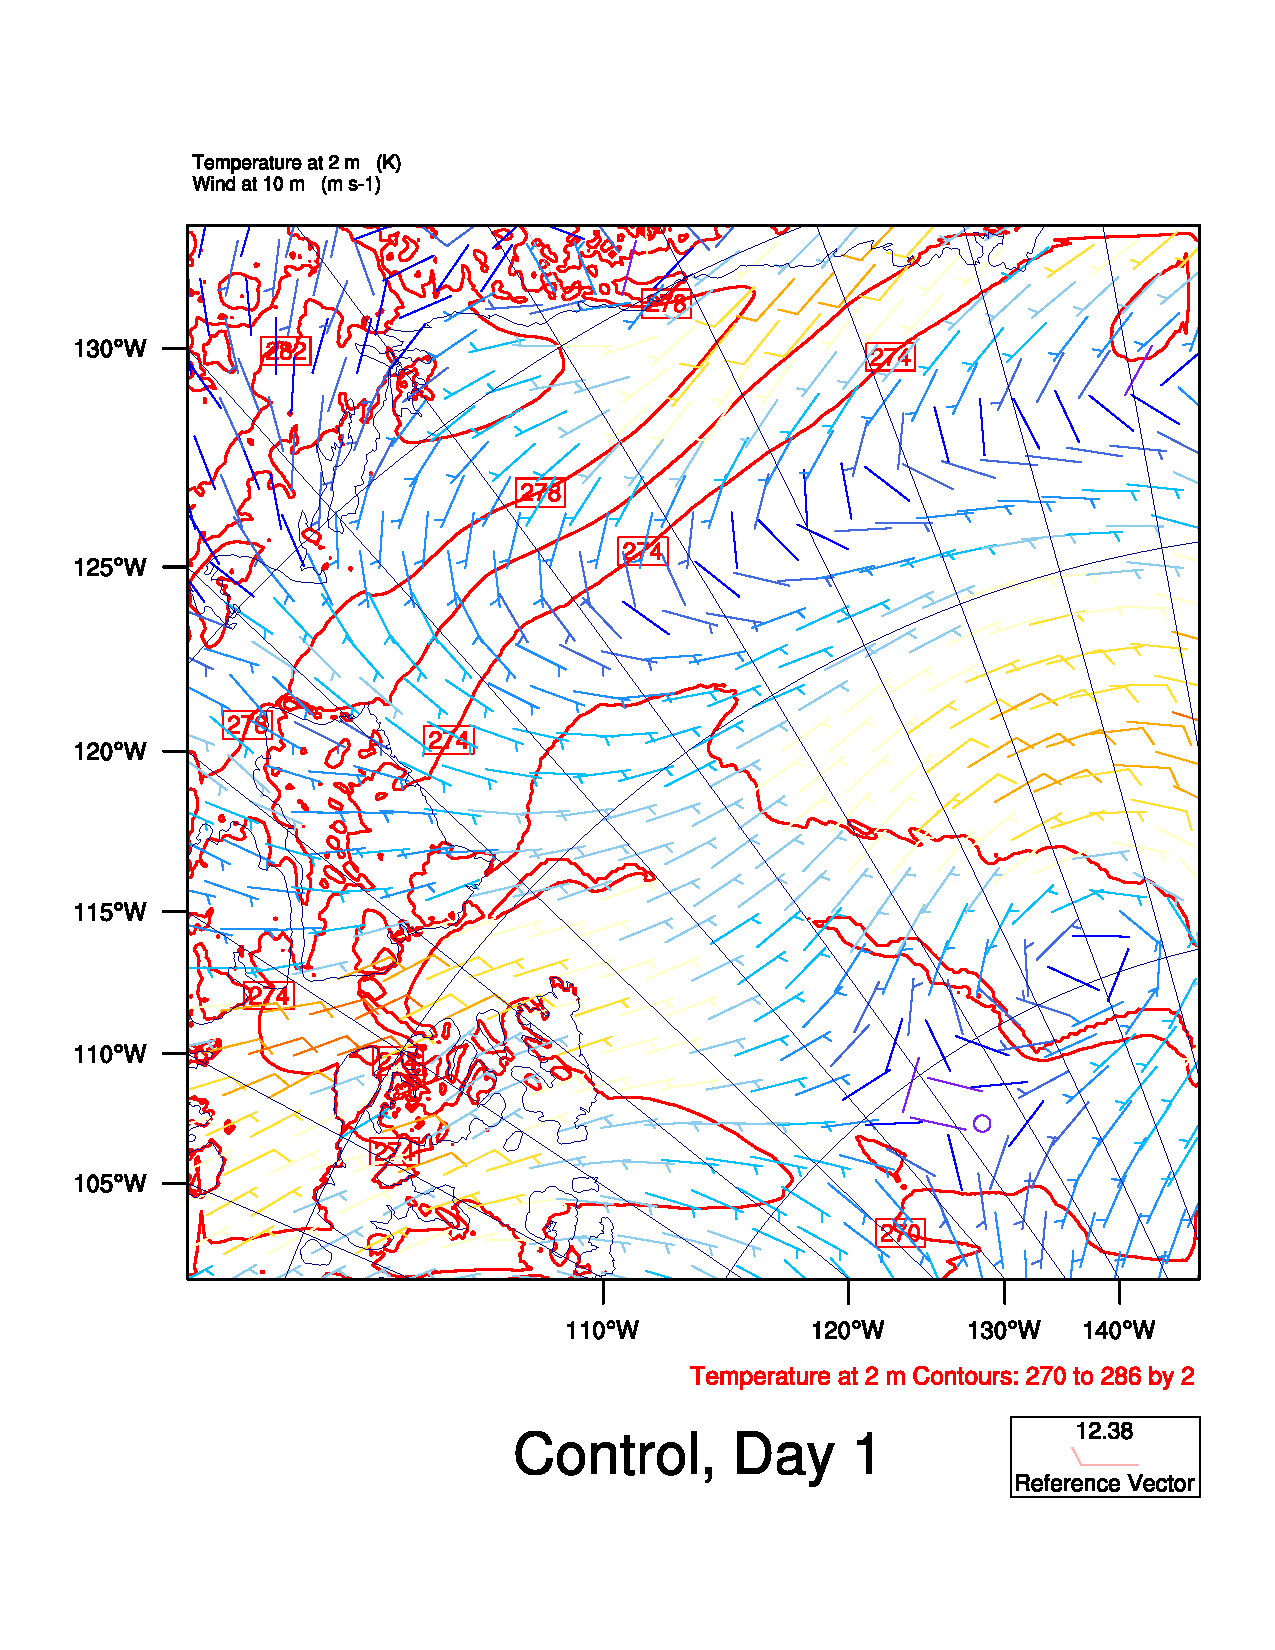
\includegraphics[width=\textwidth]{results/control/T2UV10_Control_Day1.pdf}
        \caption{Day 1}
        \label{subfig:weather_cont_day1}
    \end{subfigure}
    \begin{subfigure}{0.48\textwidth}
        \centering
        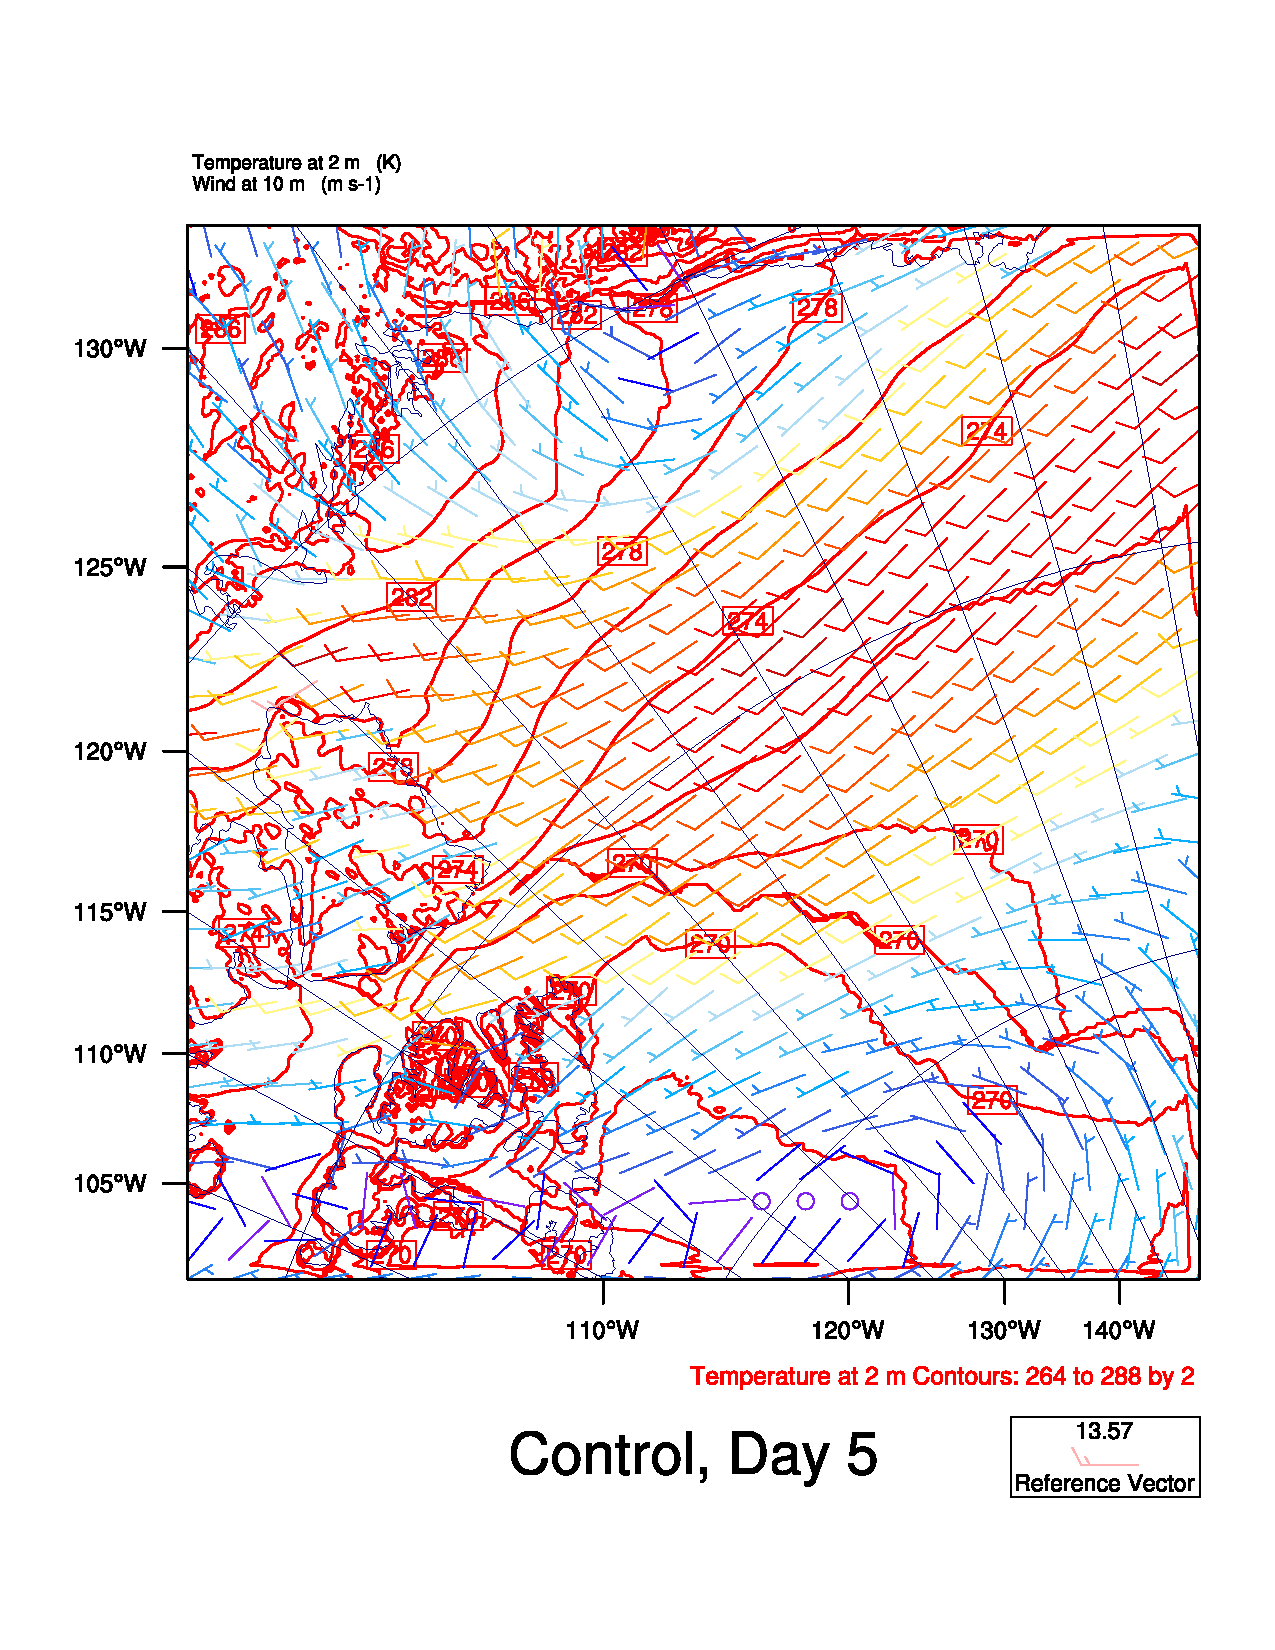
\includegraphics[width=\textwidth]{results/control/T2UV10_Control_Day5.pdf}
        \caption{Day 5}
        \label{subfig:weather_cont_day5}
    \end{subfigure}
    \caption{The temperature and wind pattern for days 1 and 5, from the control run. The temperature at 2~m height is represented by red contour lines and the wind speed and direction at 10~m height is shown by wind barbs and their color, where red indicates higher wind speed and blue indicates lower. The shortest tails on the wind barbs indicate a wind speed of 5~m/s and the longest indicate 10~m/s.}
    \label{fig:weather}
\end{figure}

By day 5 the wind direction has changed to south-easterly, see figure~\ref{subfig:weather_cont_day5}, and the clouds in the cross section, figure~\ref{subfig:cross_LWC_Day5} are low stratus over the sea ice, and there is also some thin cloud formation at the mountain, probably formed by weaker orographic lifting. There is no IWC in the section for day 5 (not shown).

\begin{figure}
    \centering
    \begin{subfigure}{0.48\textwidth}
        \centering
        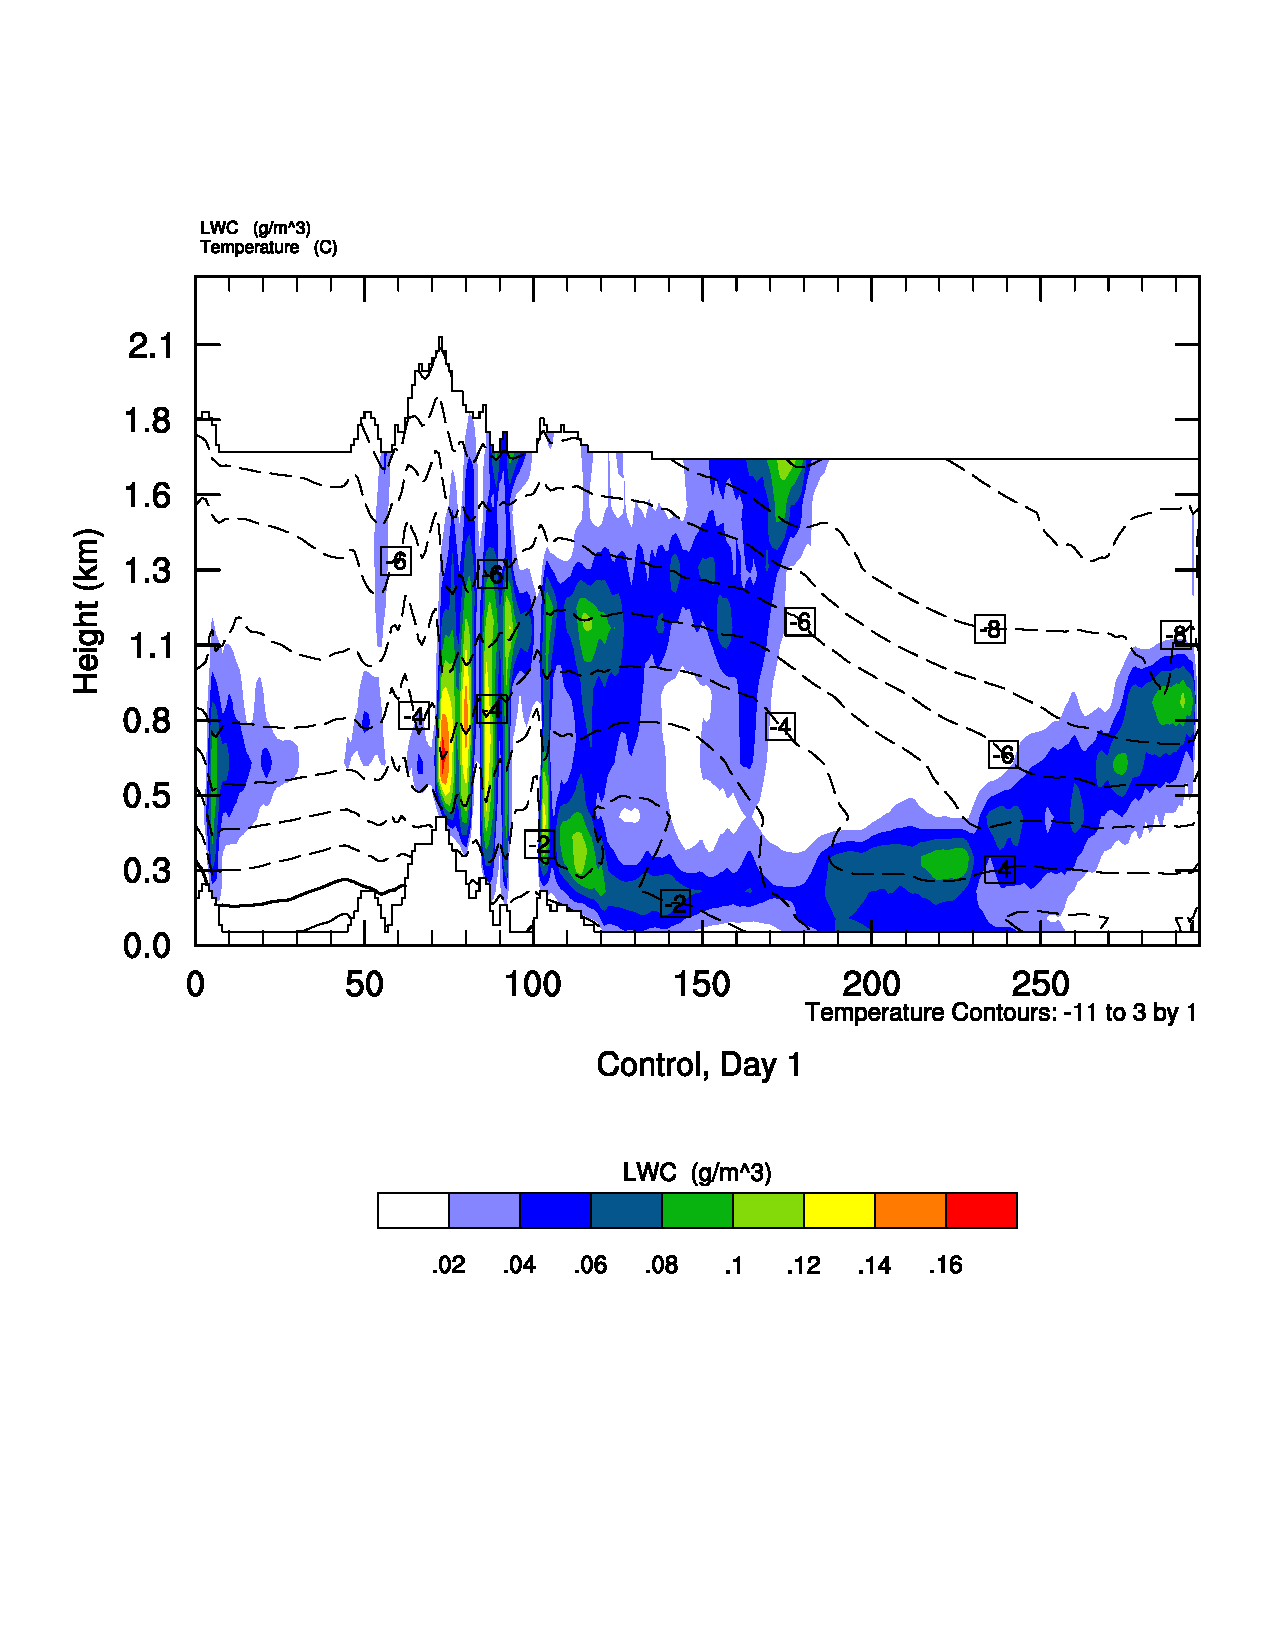
\includegraphics[width=\textwidth]{results/control/crossSec_LWC_Control_Day1.pdf}
        \caption{LWC and temperature, day 1.}
        \label{subfig:cross_LWC_day1}
    \end{subfigure}
    \begin{subfigure}{0.48\textwidth}
        \centering
        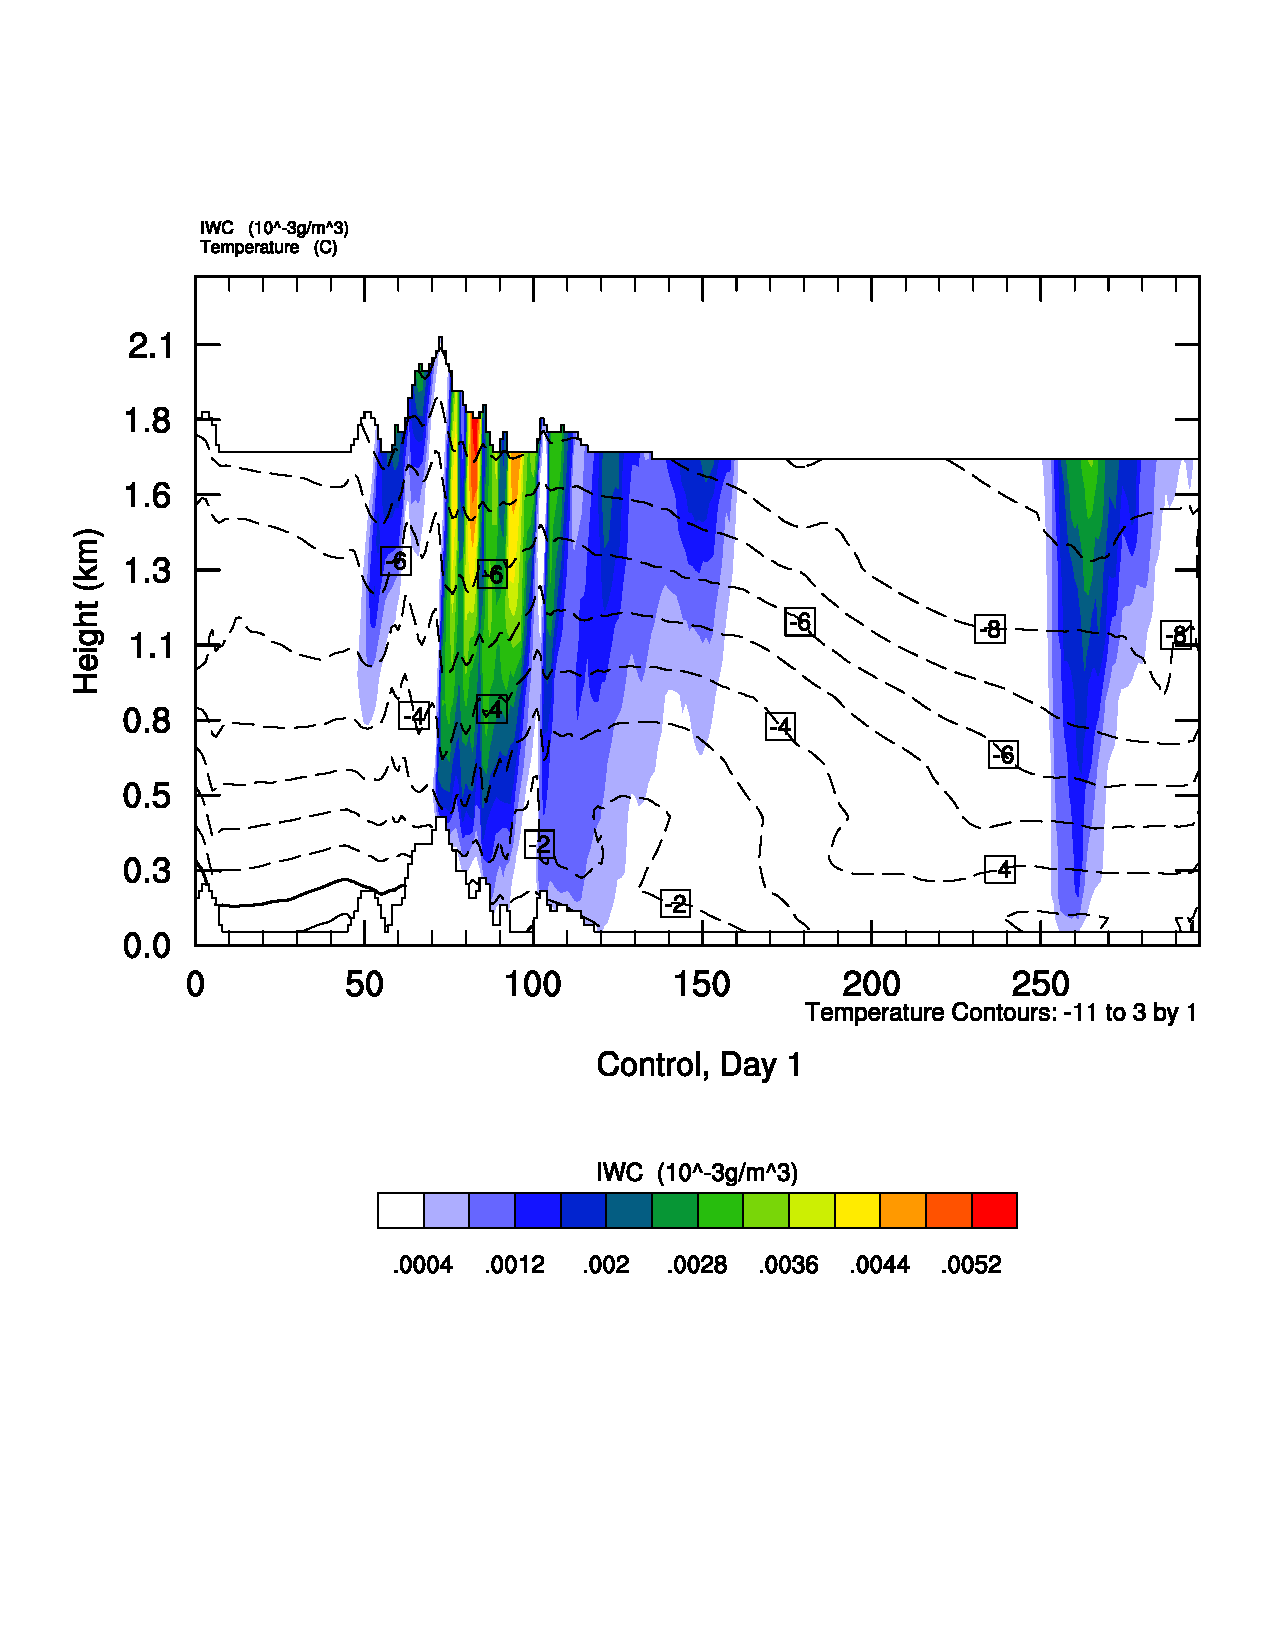
\includegraphics[width=\textwidth]{results/control/crossSec_IWC_Control_Day1.pdf}
        \caption{IWC and temperature, day1.}
        \label{subfig:cross_IWC_day1}
    \end{subfigure}
    
    \begin{subfigure}{0.48\textwidth}
        \centering
        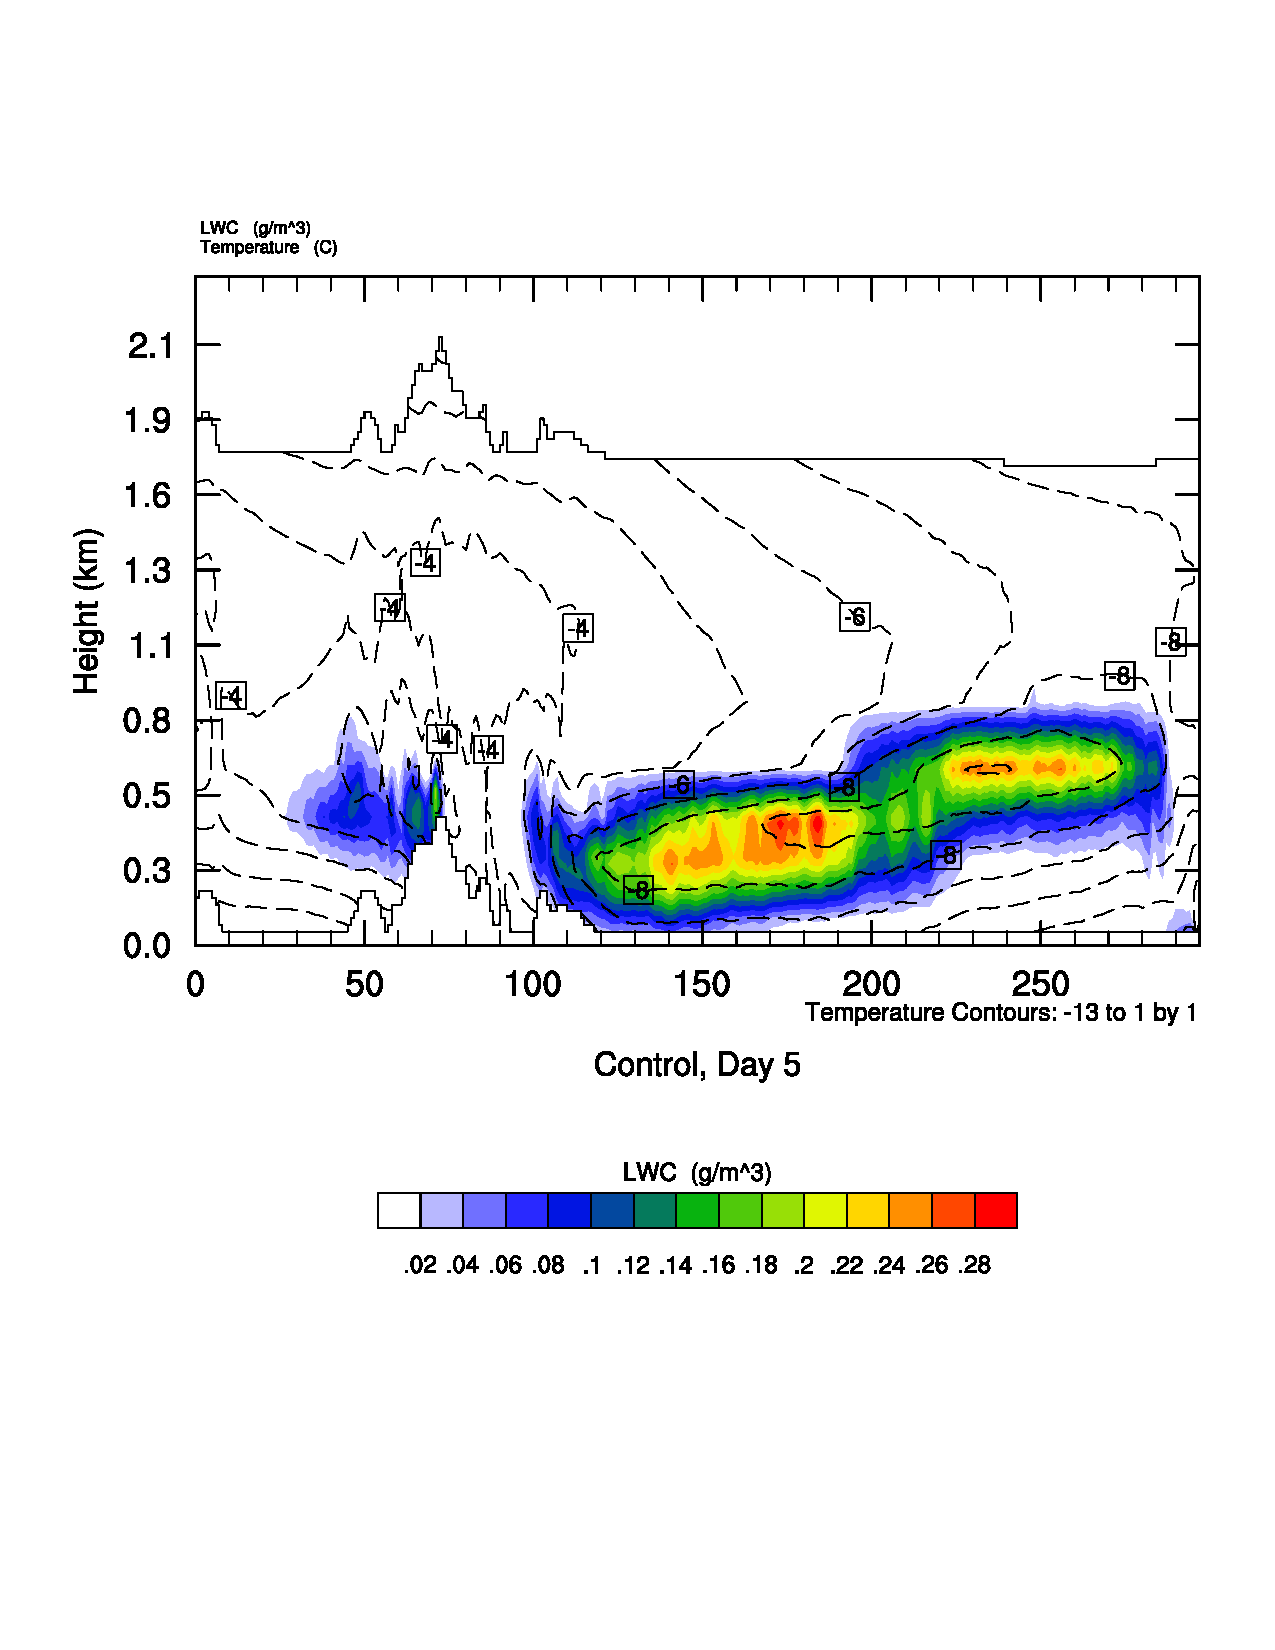
\includegraphics[width=\textwidth]{results/control/crossSec_LWC_Control_Day5.pdf}
        \caption{LWC and temperature, day 5.}
        \label{subfig:cross_LWC_Day5}
    \end{subfigure}
    \begin{subfigure}{0.48\textwidth}
        \centering
        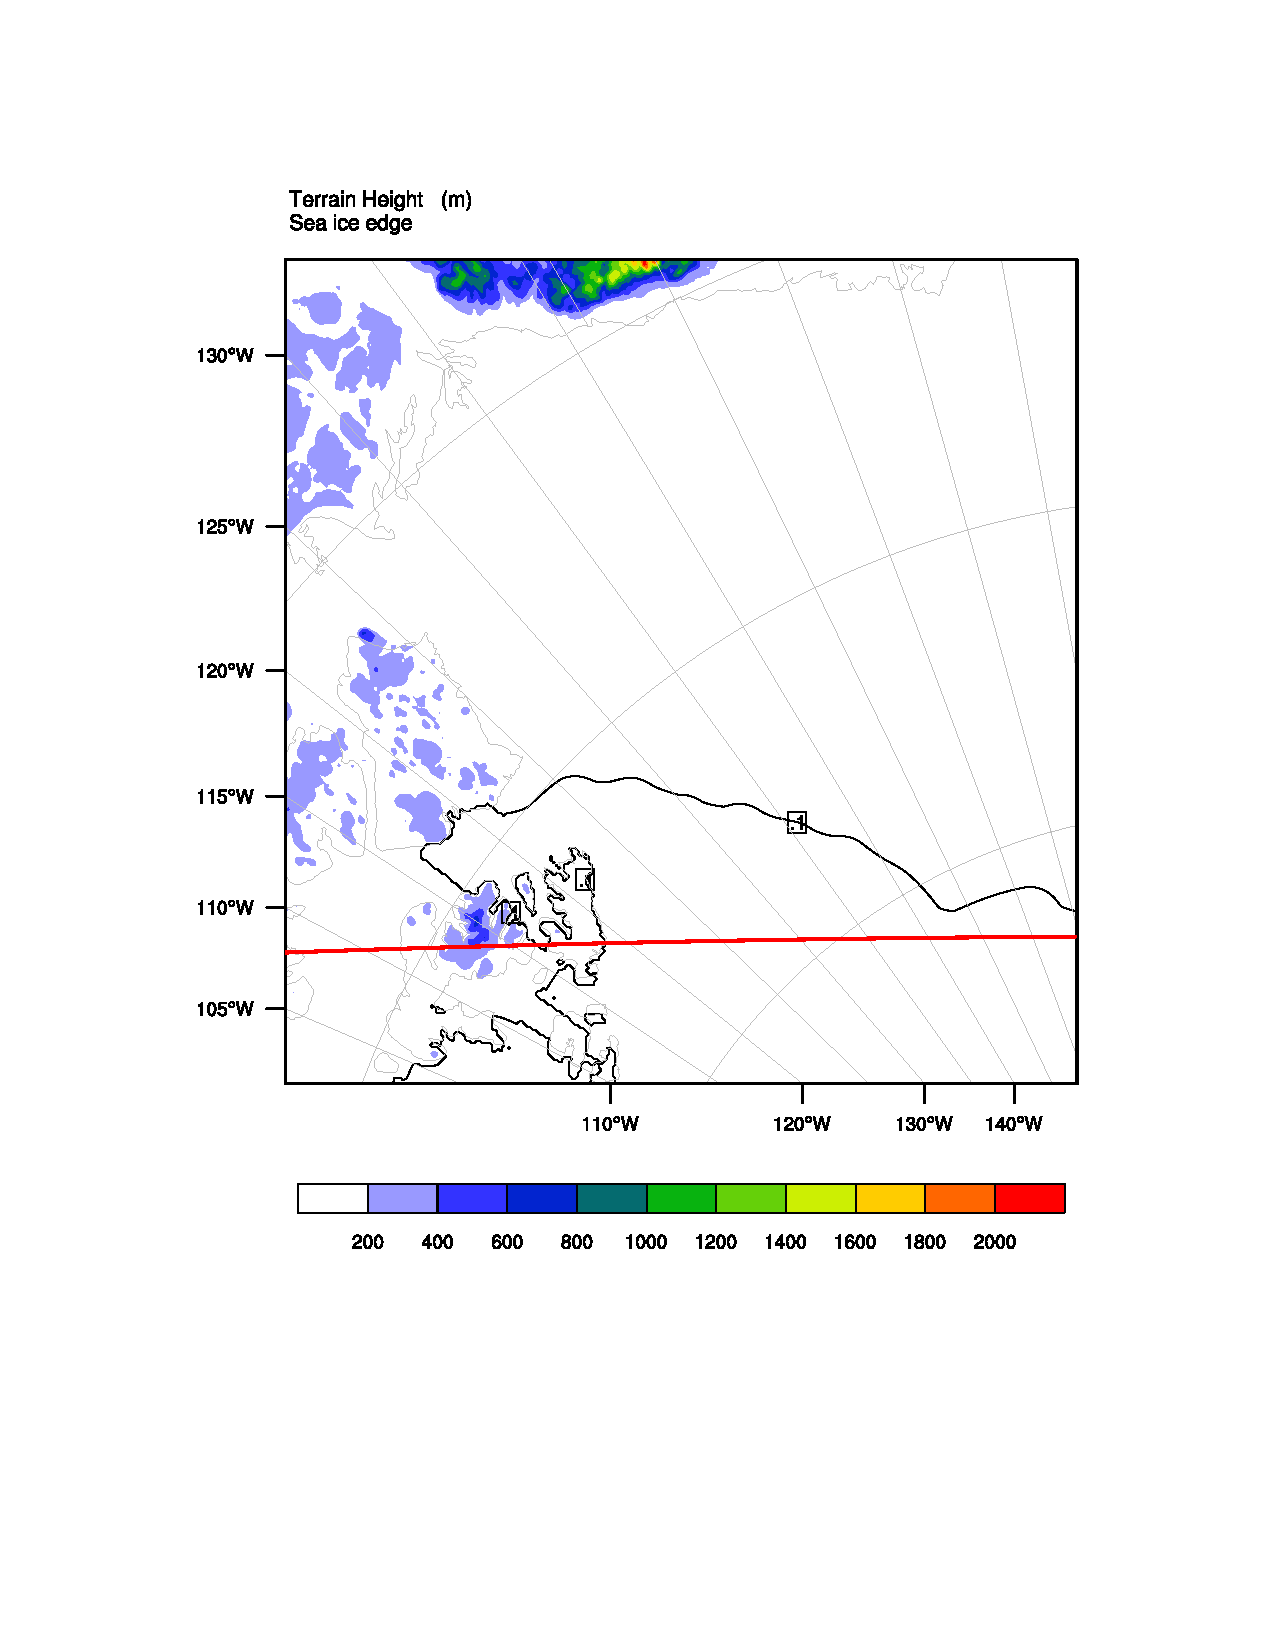
\includegraphics[width=\textwidth]{results/control/crossSec_line.pdf}
        \caption{Line over which the vertical cross sections are made.}
        \label{subfig:cross_line}
    \end{subfigure}
    \caption{Vertical cross sections of averaged liquid ($\text{g/m}^3$) and ice  ($\text{mg/m}^3$) water content, as filled contours, with temperature ($\degree\text{C}$) as dashed contours, from the control run, for days 1 and 5. LWC and IWC for day 1 are shown in figures~\ref{subfig:cross_LWC_day1} and~\ref{subfig:cross_IWC_day1} respectively. Figure~\ref{subfig:cross_LWC_Day5} shows the LWC for day 5. The IWC on day 5 was 0 in the section and is not shown. Figure~\ref{subfig:cross_line} shows a map of the area with the ice edge as a black contour line. The terrain height is represented by filled contours and the red line over the sea ice is the line over which the cross sections are made.}
    \label{fig:sections}
\end{figure}

The LWP for days 1 and 5 are shown in figure~\ref{subfig:LWPr1Day1} and~\ref{subfig:LWPr1Day5} with the CDNC~(\ref{subfig:cdnc_cont_Day1} and~\ref{subfig:cdnc_cont_Day5}) and $r_e$~(\ref{subfig:recloud_r1Day1} and~\ref{subfig:recloud_r1Day5}). One can clearly see that the LWP and the CDNC have similar pattern, which is expected based on equation~\ref{eqn:LWC}. The pattern in $r_e$ also fits quite well with that of LWP, meaning that larger droplets contain more water.

The fluxes of both SW and LW radiation at both downward at the surface and upward at the top of the atmosphere (TOA) may be partly explained by the clouds (@utdyp, Jon egill spør: Hvordan det?), through looking at the LWP. Figures~\ref{fig:radiation_r1Day1} and~\ref{fig:radiation_r1Day5} show the downward SW and LW at the surface and upward at TOA for days 1 and 5 respectively.

The heat fluxes upward at the surface, latent heat (LH) and sensible heat (SH), are also of interest when studying clouds in the Arctic. The fluxes are shown in figure~\ref{fig:surface_fluxes_r1} for days 1 and 5. Notice that the LH and SH are lower over the sea ice for both days 1 and 5. This because the sea ice is colder than the ocean, and works as a lid over that part of the ocean, not letting all the heat and water vapor out.


%---------- LWP control run, days 1 and 5
\begin{figure}
    \centering
    \begin{subfigure}{0.40\textwidth}
        \centering
        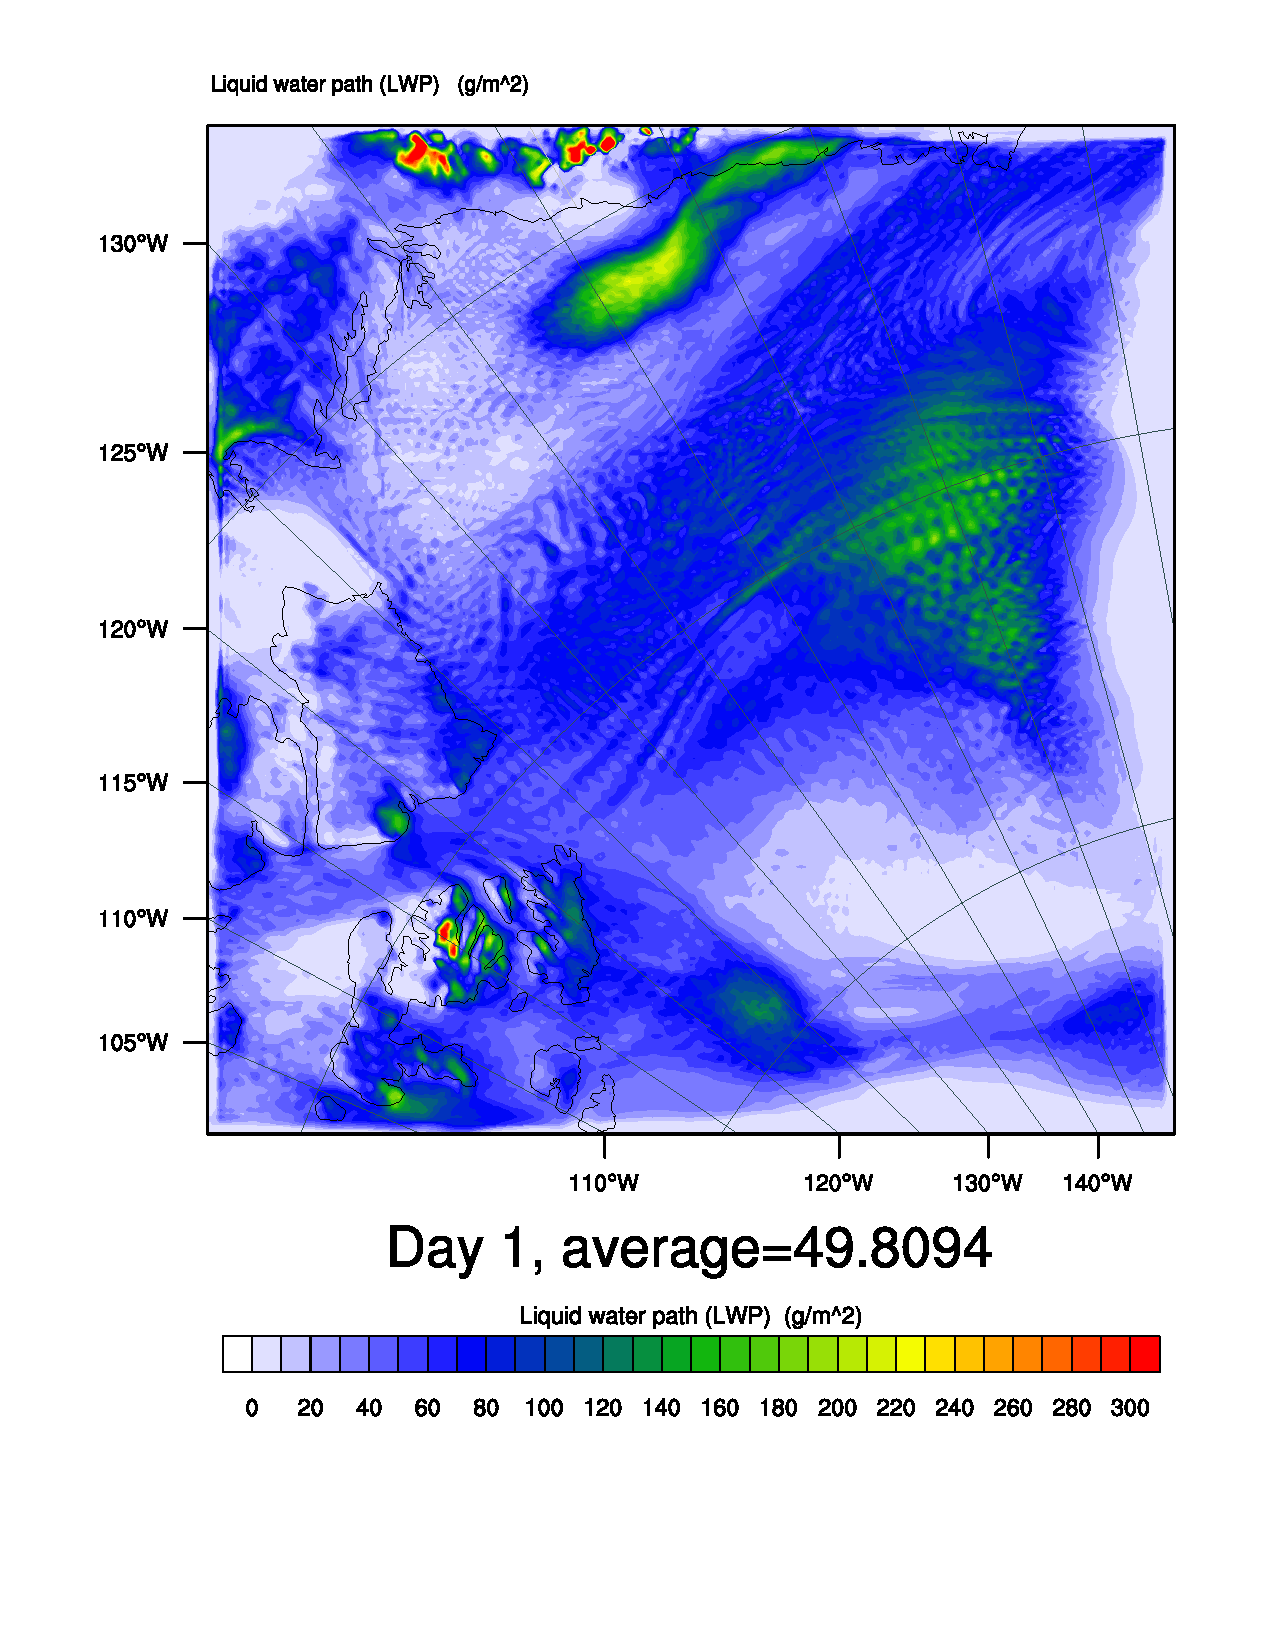
\includegraphics[width=\textwidth]{results/control/LWP_Day1.pdf}
        \caption{LWP day 1.}
        \label{subfig:LWPr1Day1}
    \end{subfigure}
    \begin{subfigure}{0.40\textwidth}
        \centering
        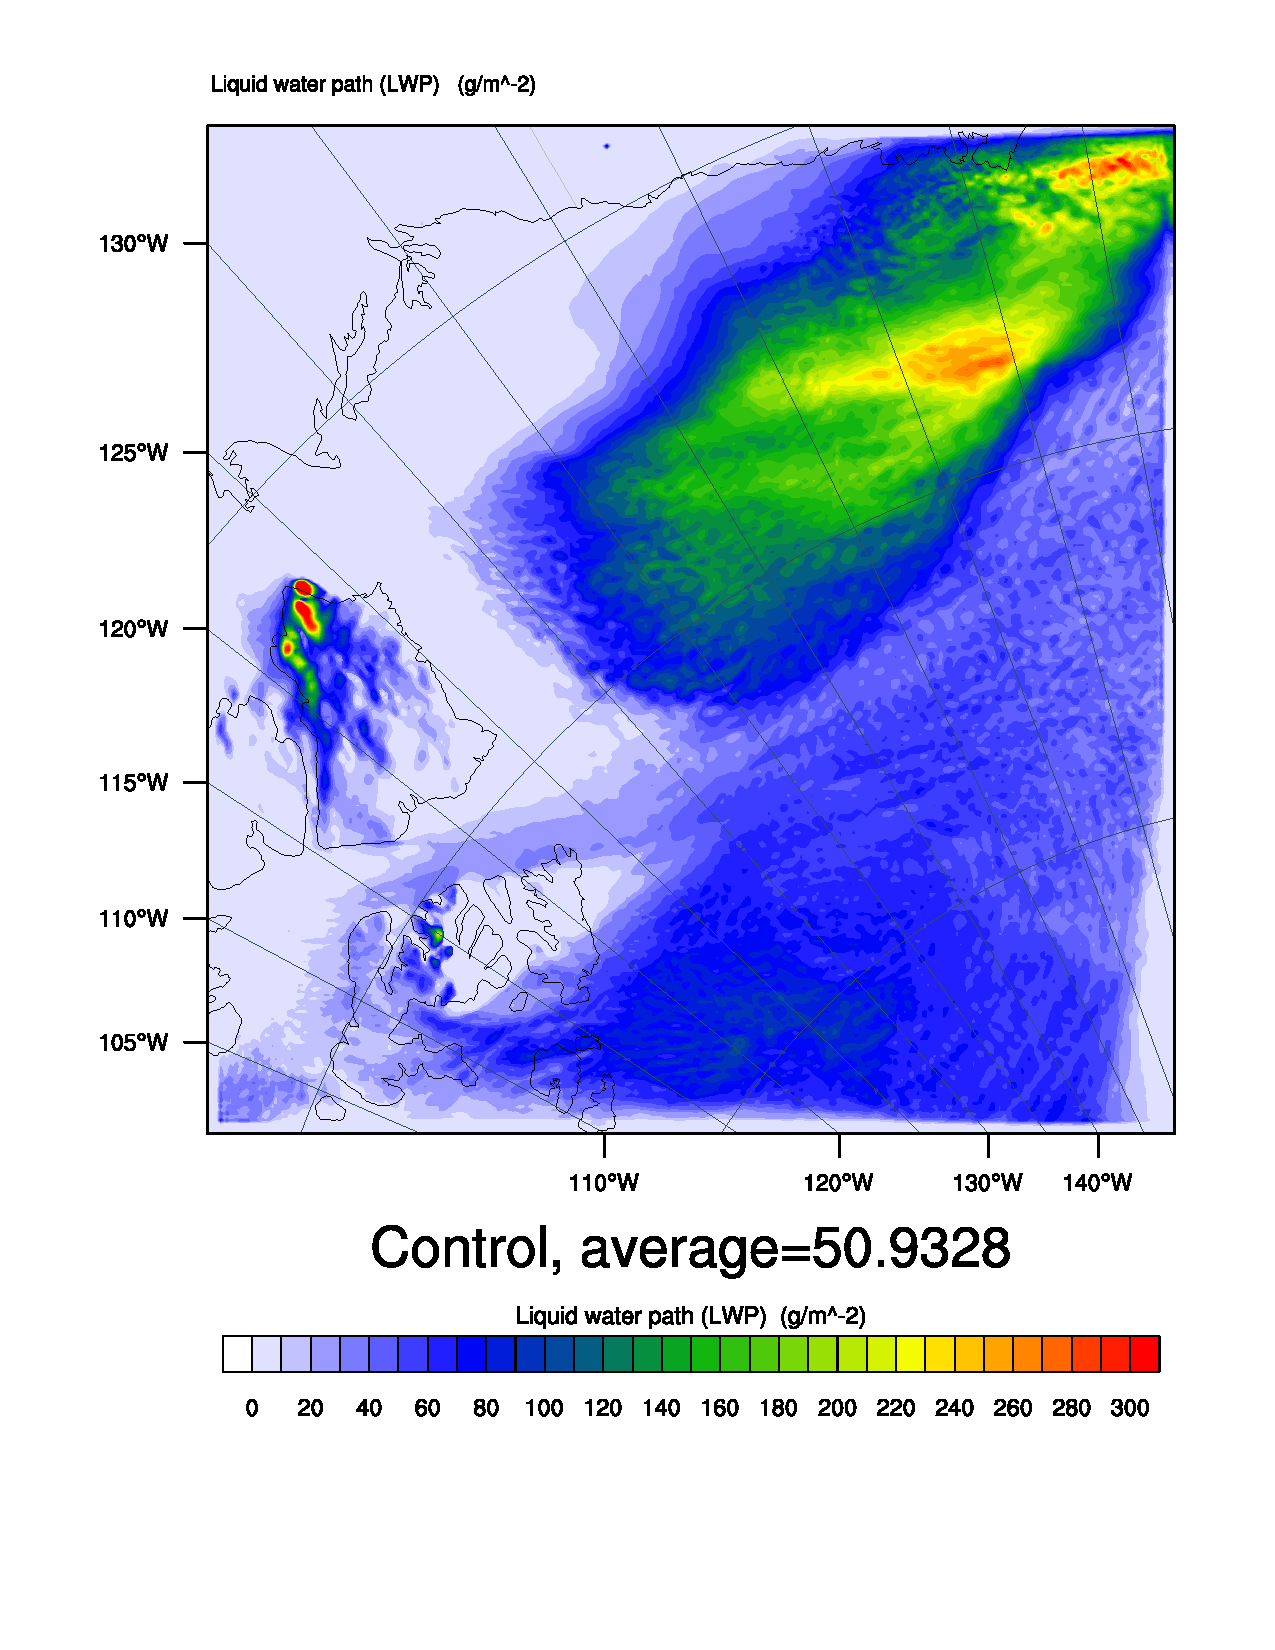
\includegraphics[width=\textwidth]{results/control/LWP_Day5.pdf}
        \caption{LWP day 5.}
        \label{subfig:LWPr1Day5}
    \end{subfigure}

%------CDNC
	\begin{subfigure}{0.40\textwidth}
		\centering
		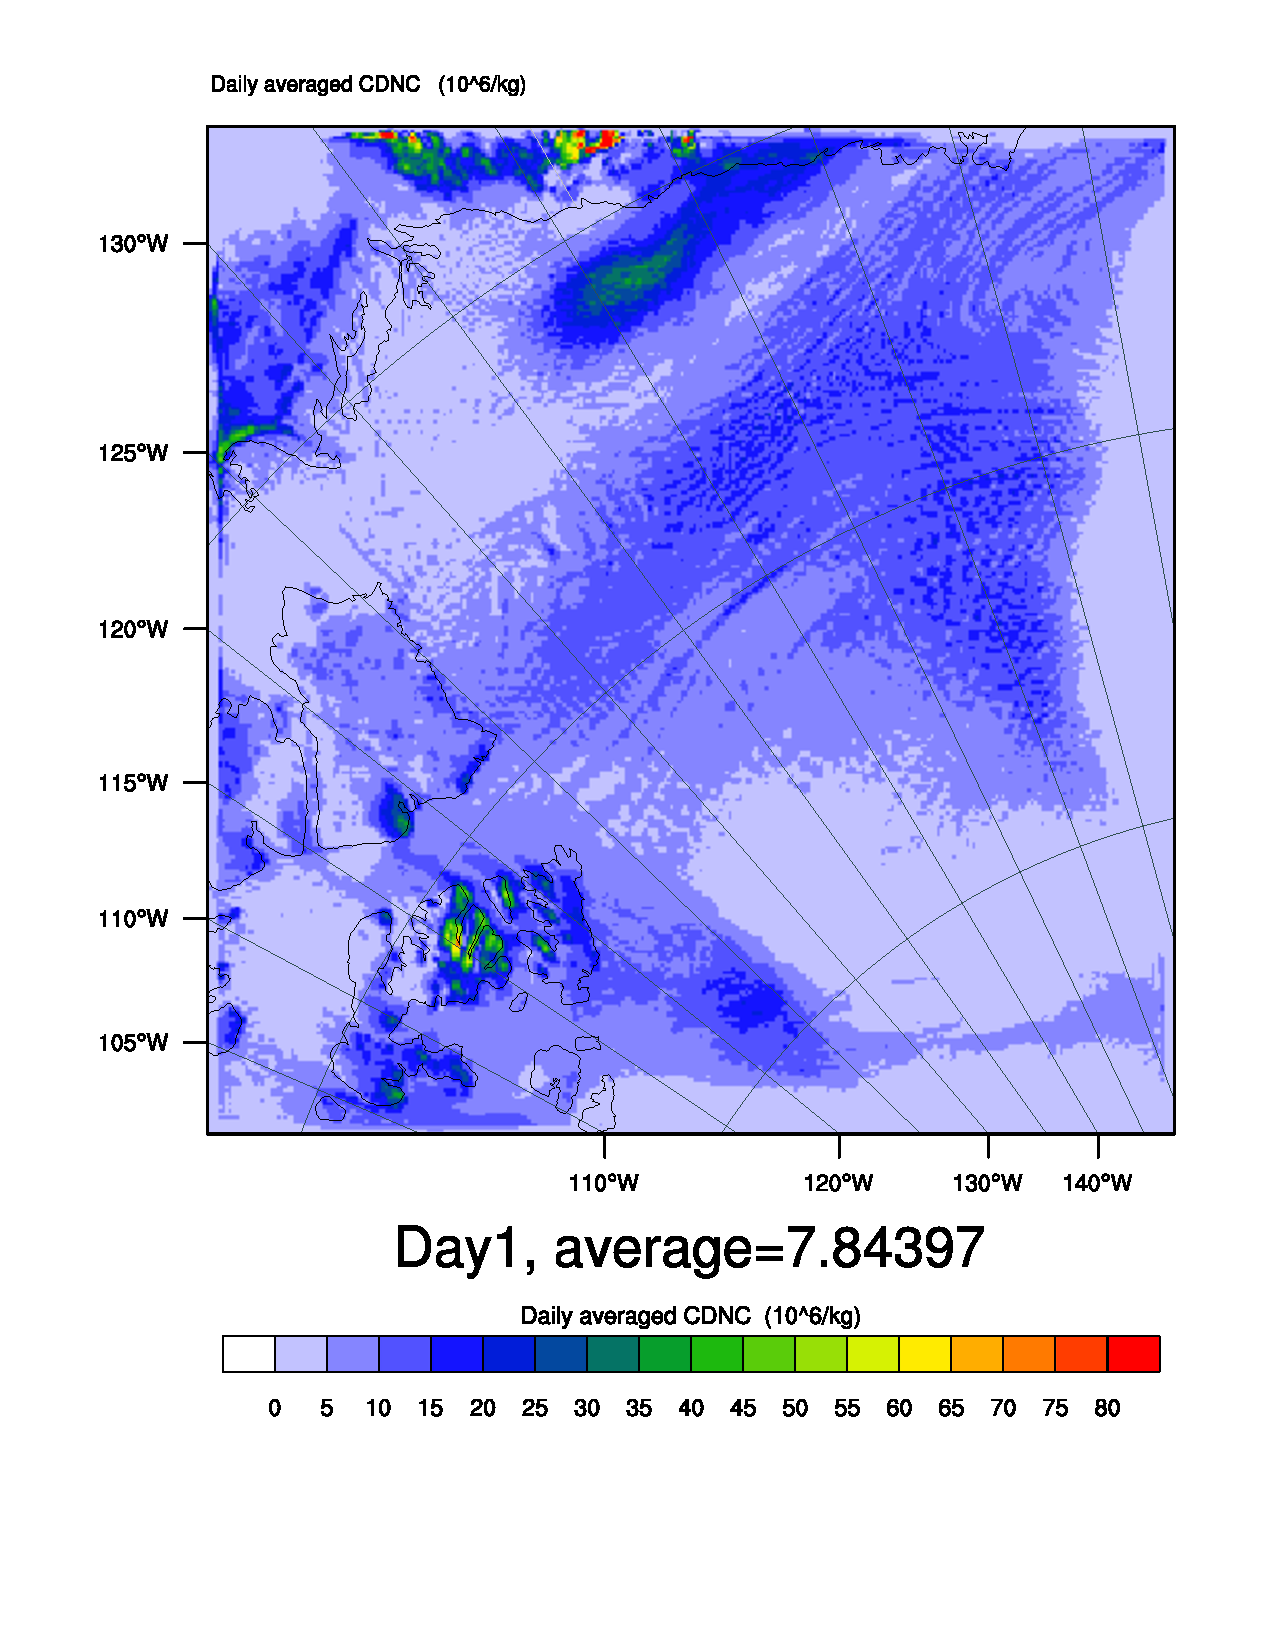
\includegraphics[width=\textwidth]{results/control/QNCLOUD_Day1.pdf}
		\caption{CDNC day 1.}
		\label{subfig:cdnc_cont_Day1}
	\end{subfigure}
	\begin{subfigure}{0.40\textwidth}
		\centering
		\includegraphics[width=\textwidth]{results/control/QNCLOUD_day5.pdf}
		\caption{CDNC day 5.}
		\label{subfig:cdnc_cont_Day5}
	\end{subfigure}
	
%----------- Effective radius, days 1 and 5
	\begin{subfigure}{0.40\textwidth}
		\centering
		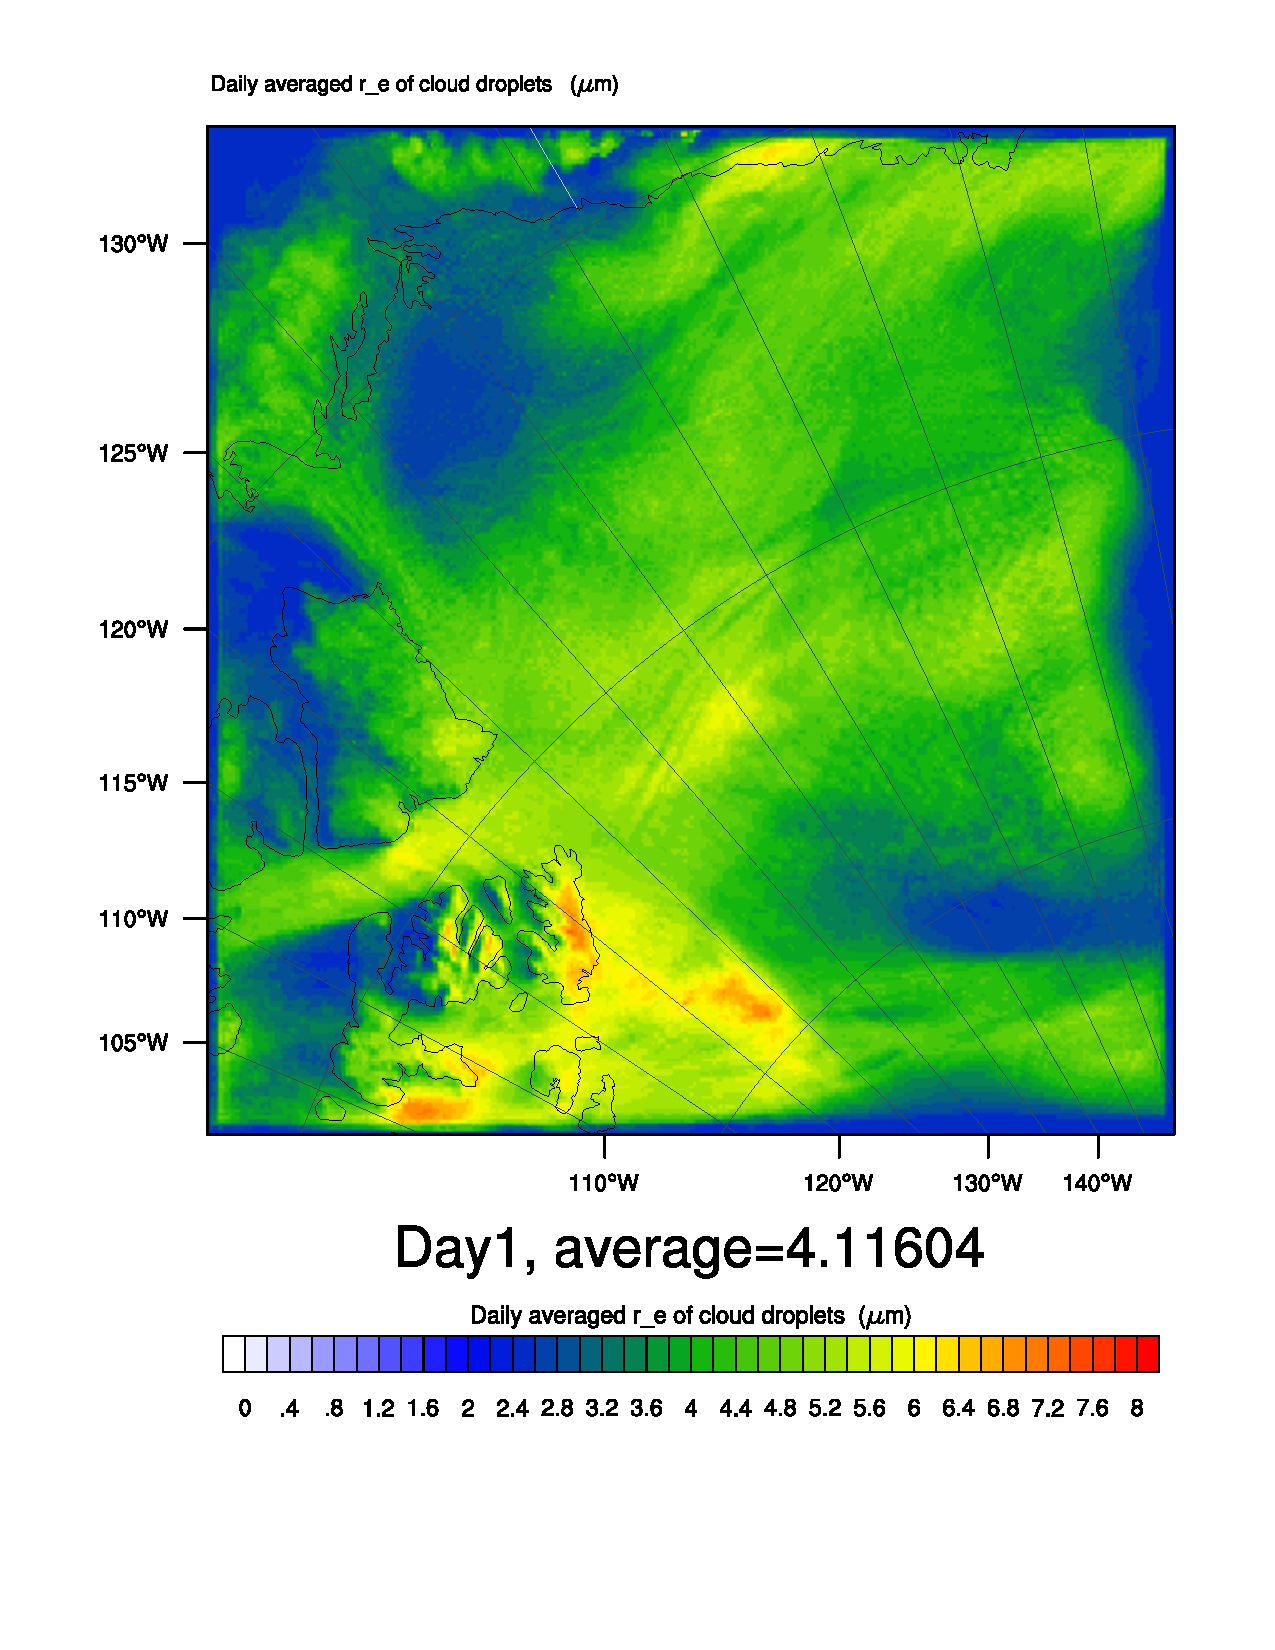
\includegraphics[width=\textwidth]{results/control/RE_CLOUD_Day1.pdf}
		\caption{$r_e$ day1.}
		\label{subfig:recloud_r1Day1}
	\end{subfigure}
	\begin{subfigure}{0.40\textwidth}
		\centering
		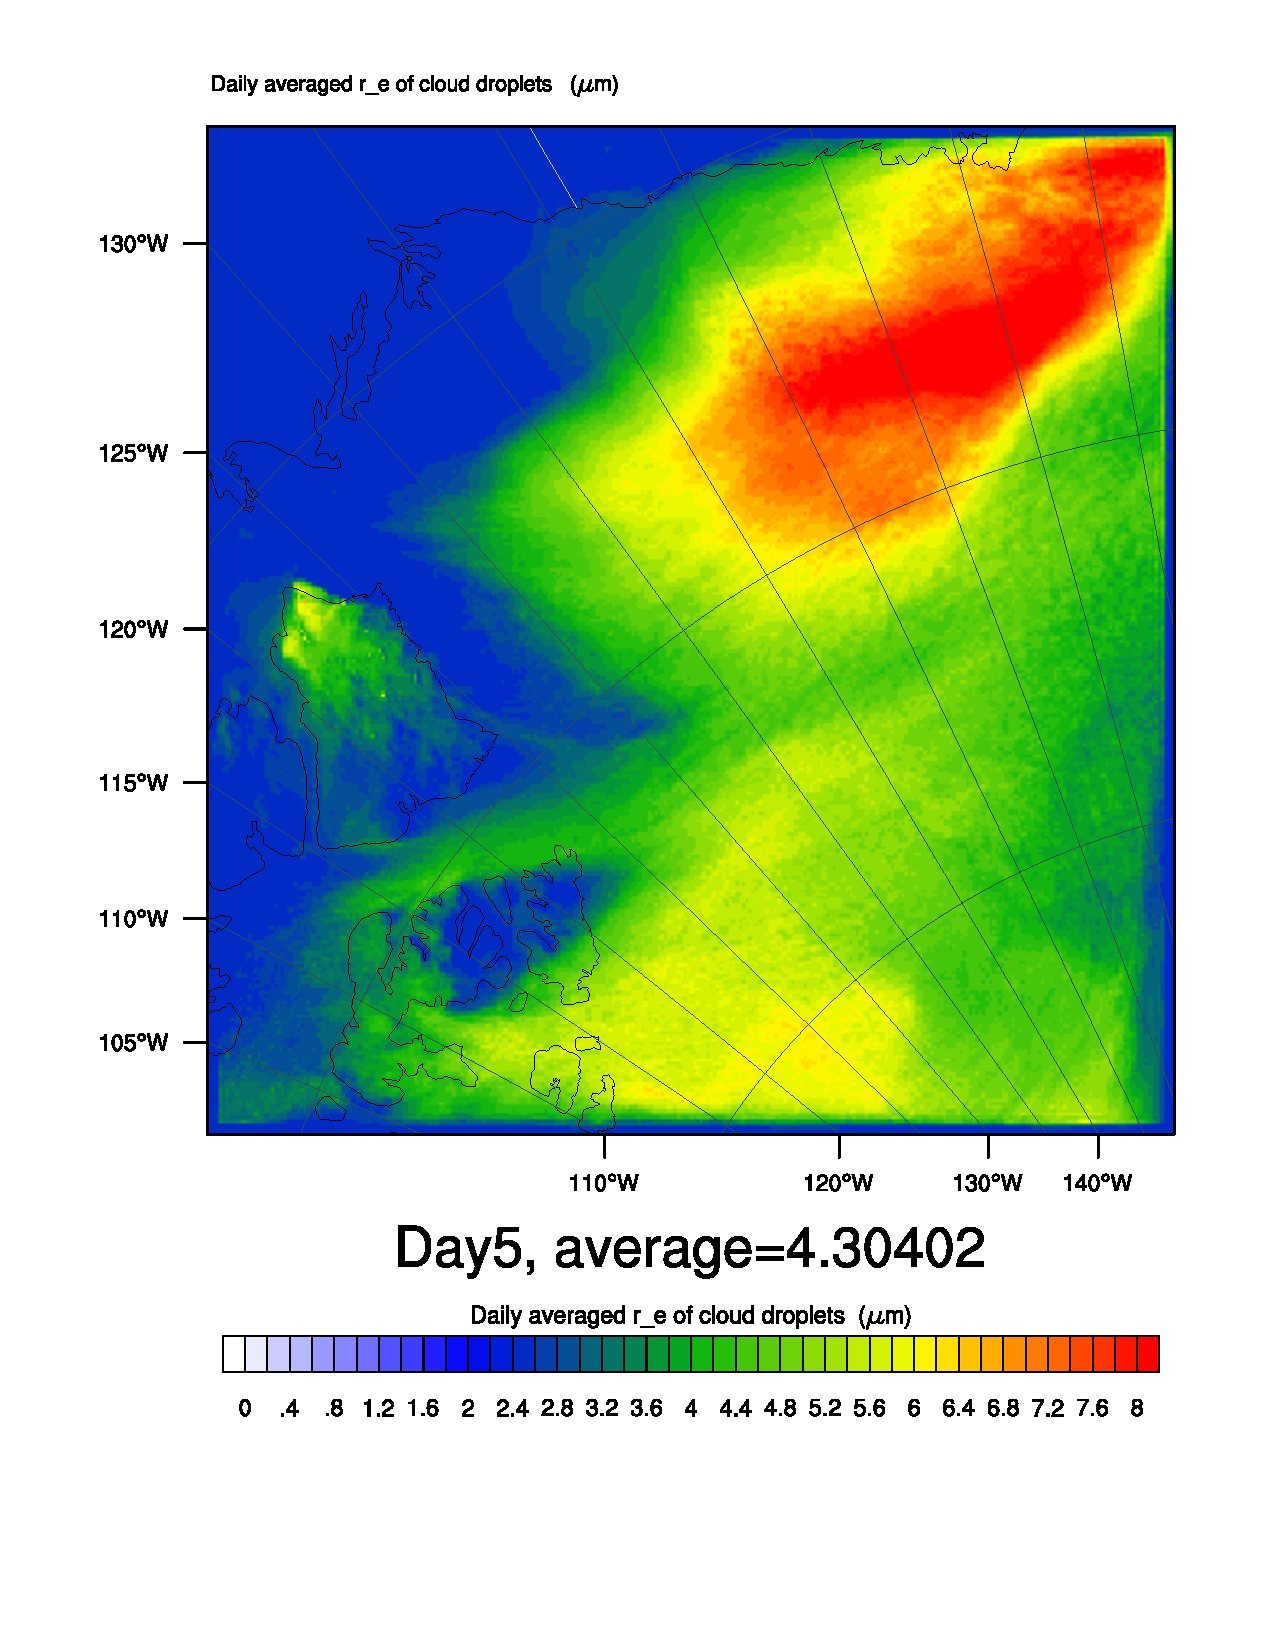
\includegraphics[width=\textwidth]{results/control/RE_CLOUD_Day5.pdf}
		\caption{$r_e$ day 5.}
		\label{subfig:recloud_r1Day5}
	\end{subfigure}
	\caption{LWP averaged in time, and CDNC and $r_e$ averaged over the lowermost 11 layers and time, for days 1 and 5. Control.}
	\label{fig:recloud_r1}
\end{figure}

%----------Radiation Day 1
\begin{figure}
\centering
	\begin{subfigure}{0.48\textwidth}
		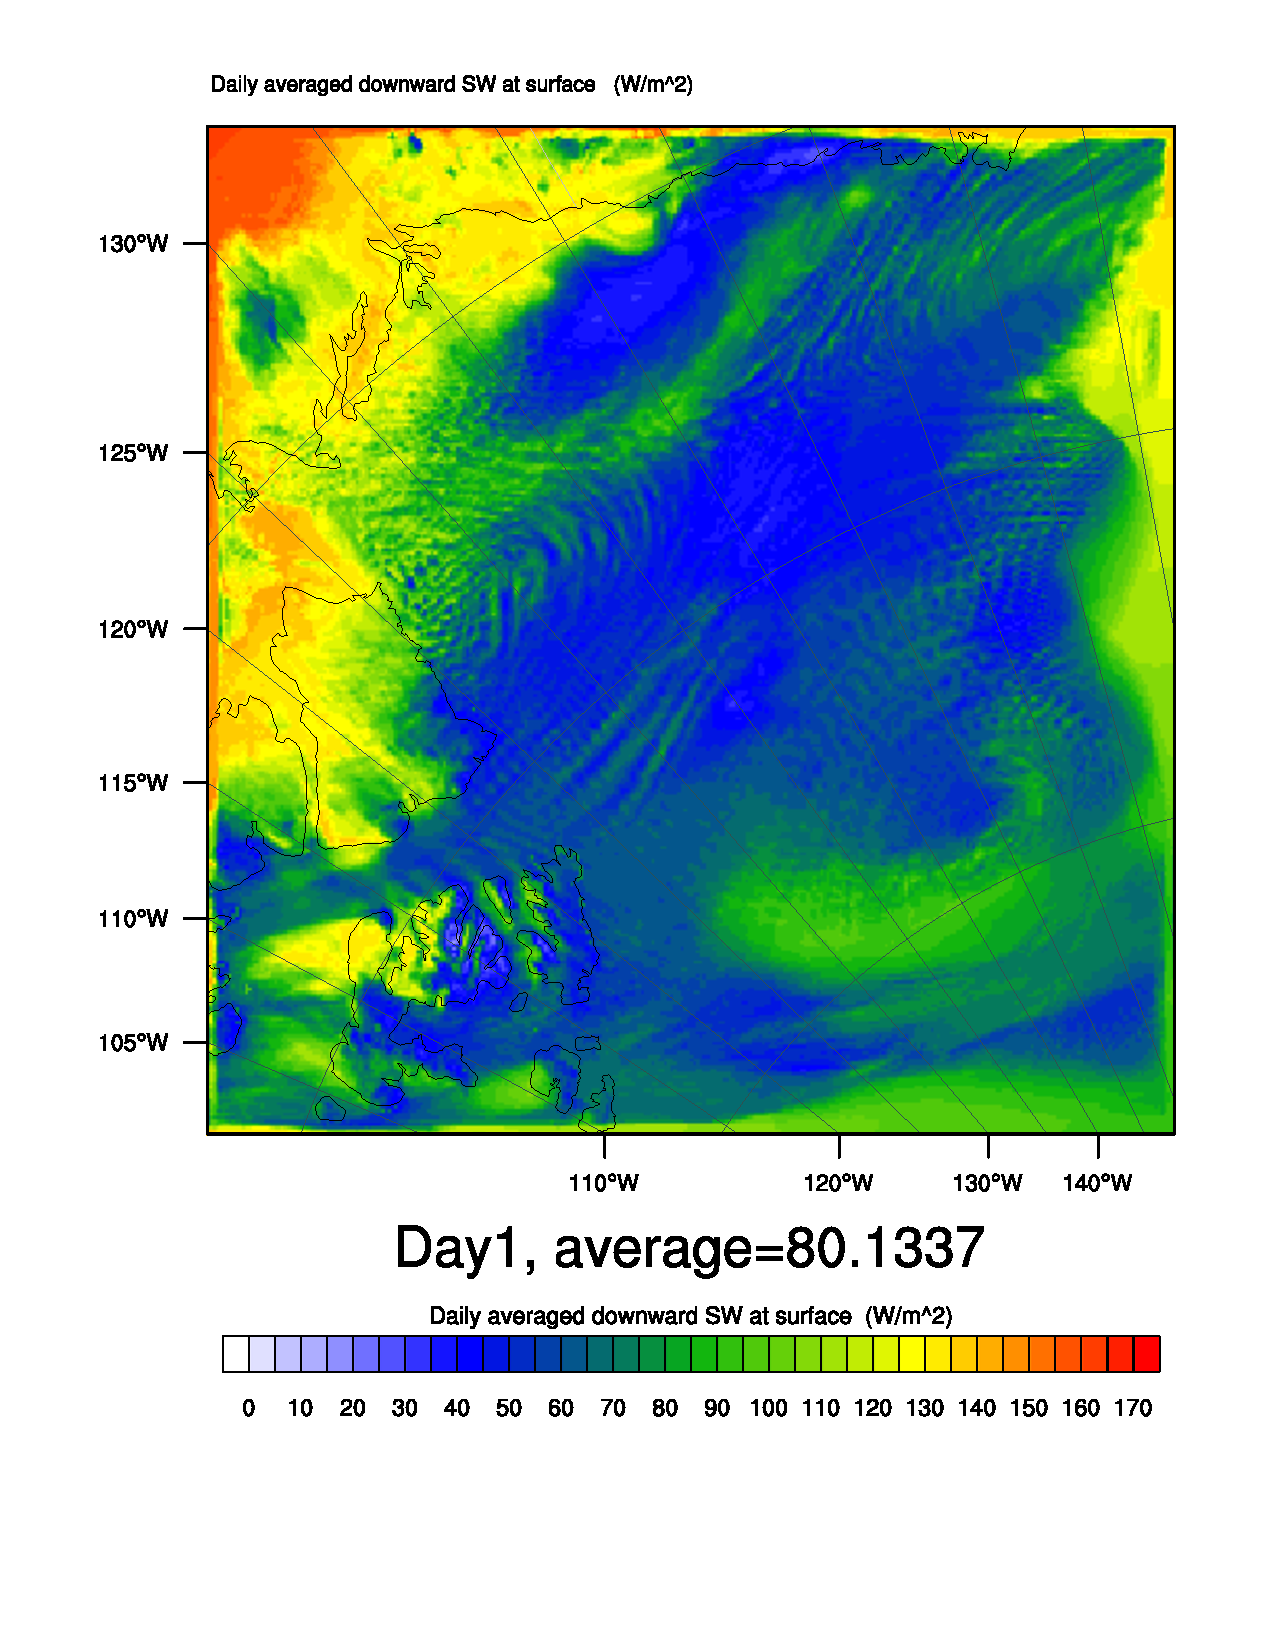
\includegraphics[width=\textwidth]{results/control/SWDOWN_Day1.pdf}
		\caption{SW down at the surface, day 1.}
		\label{subfig:swdown_r1Day1}
	\end{subfigure}
	\quad
	\begin{subfigure}{0.48\textwidth}
		\centering
		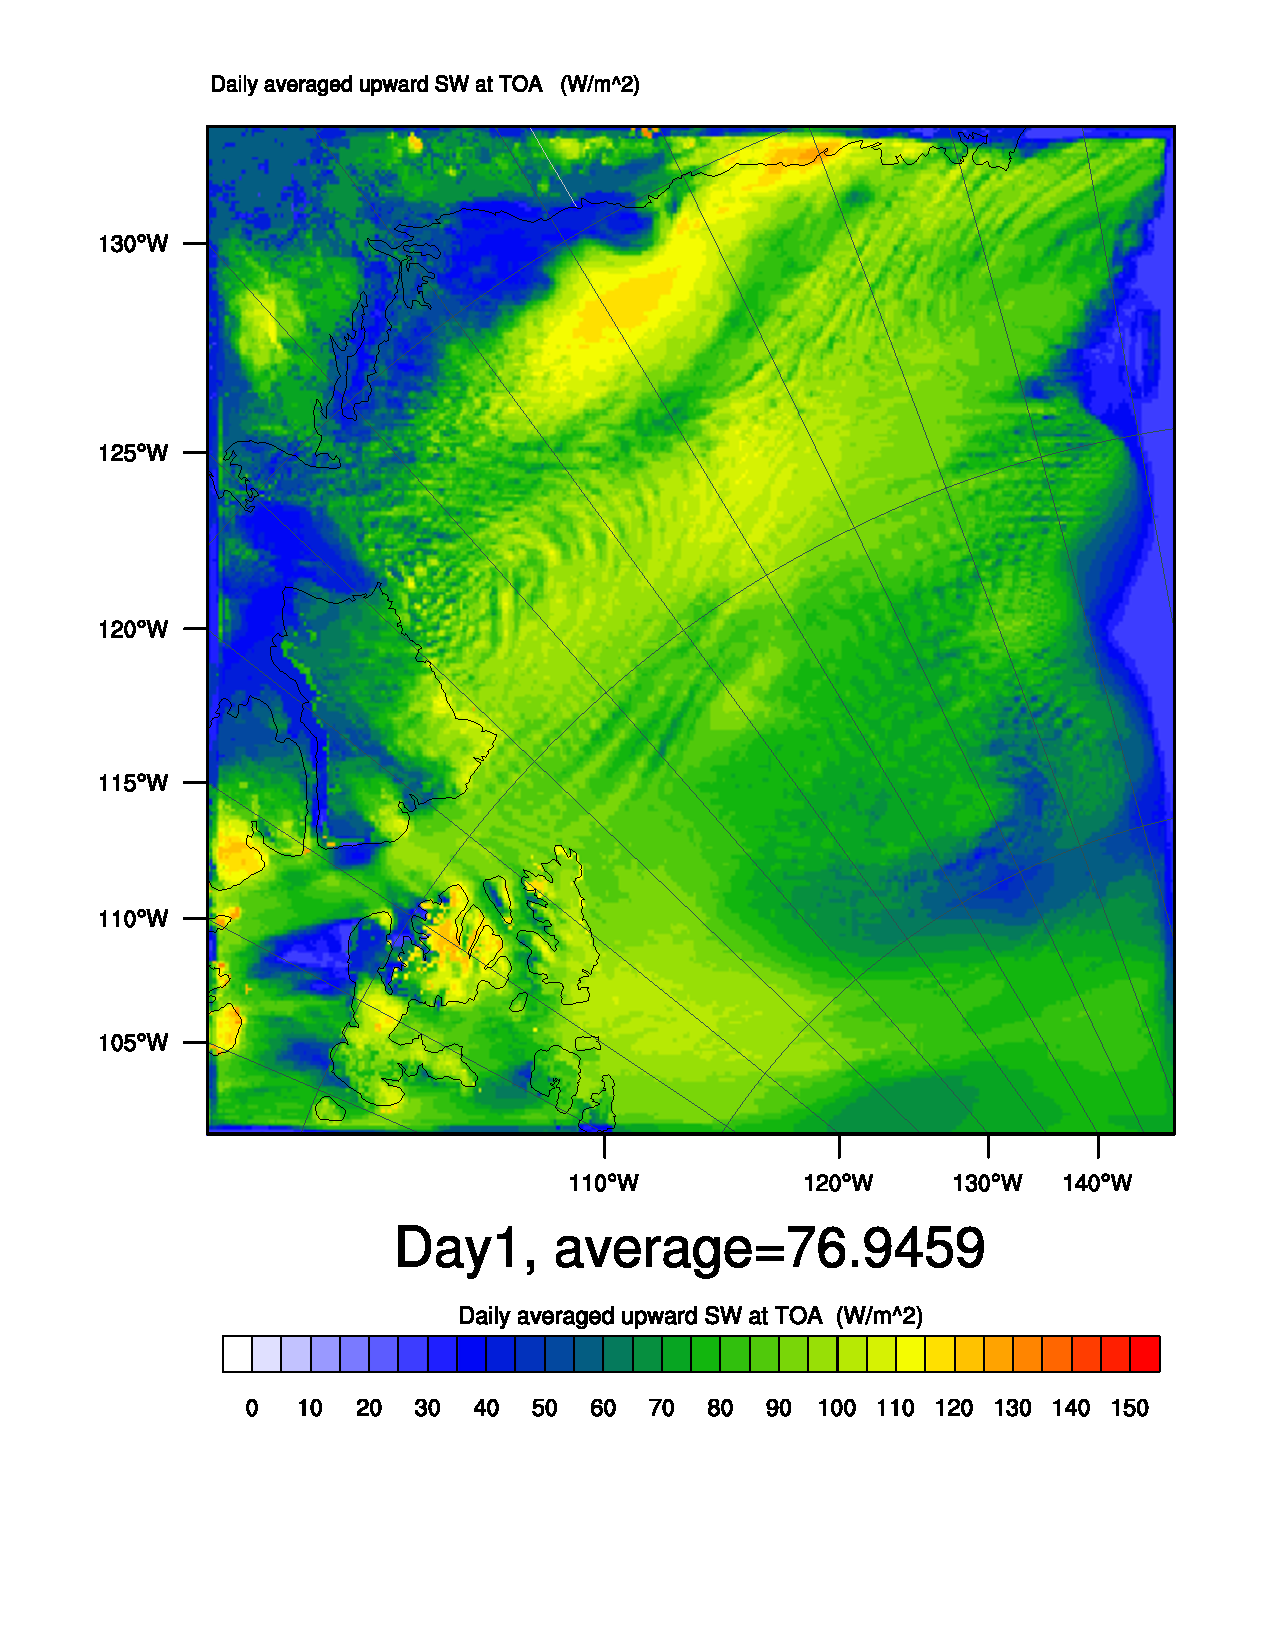
\includegraphics[width=\textwidth]{results/control/SWUPT_Day1.pdf}
		\caption{SW up at TOA, day 1.}
		\label{subfig:swup_r1Day1}
	\end{subfigure}
	
	\begin{subfigure}{0.48\textwidth}
		\centering
		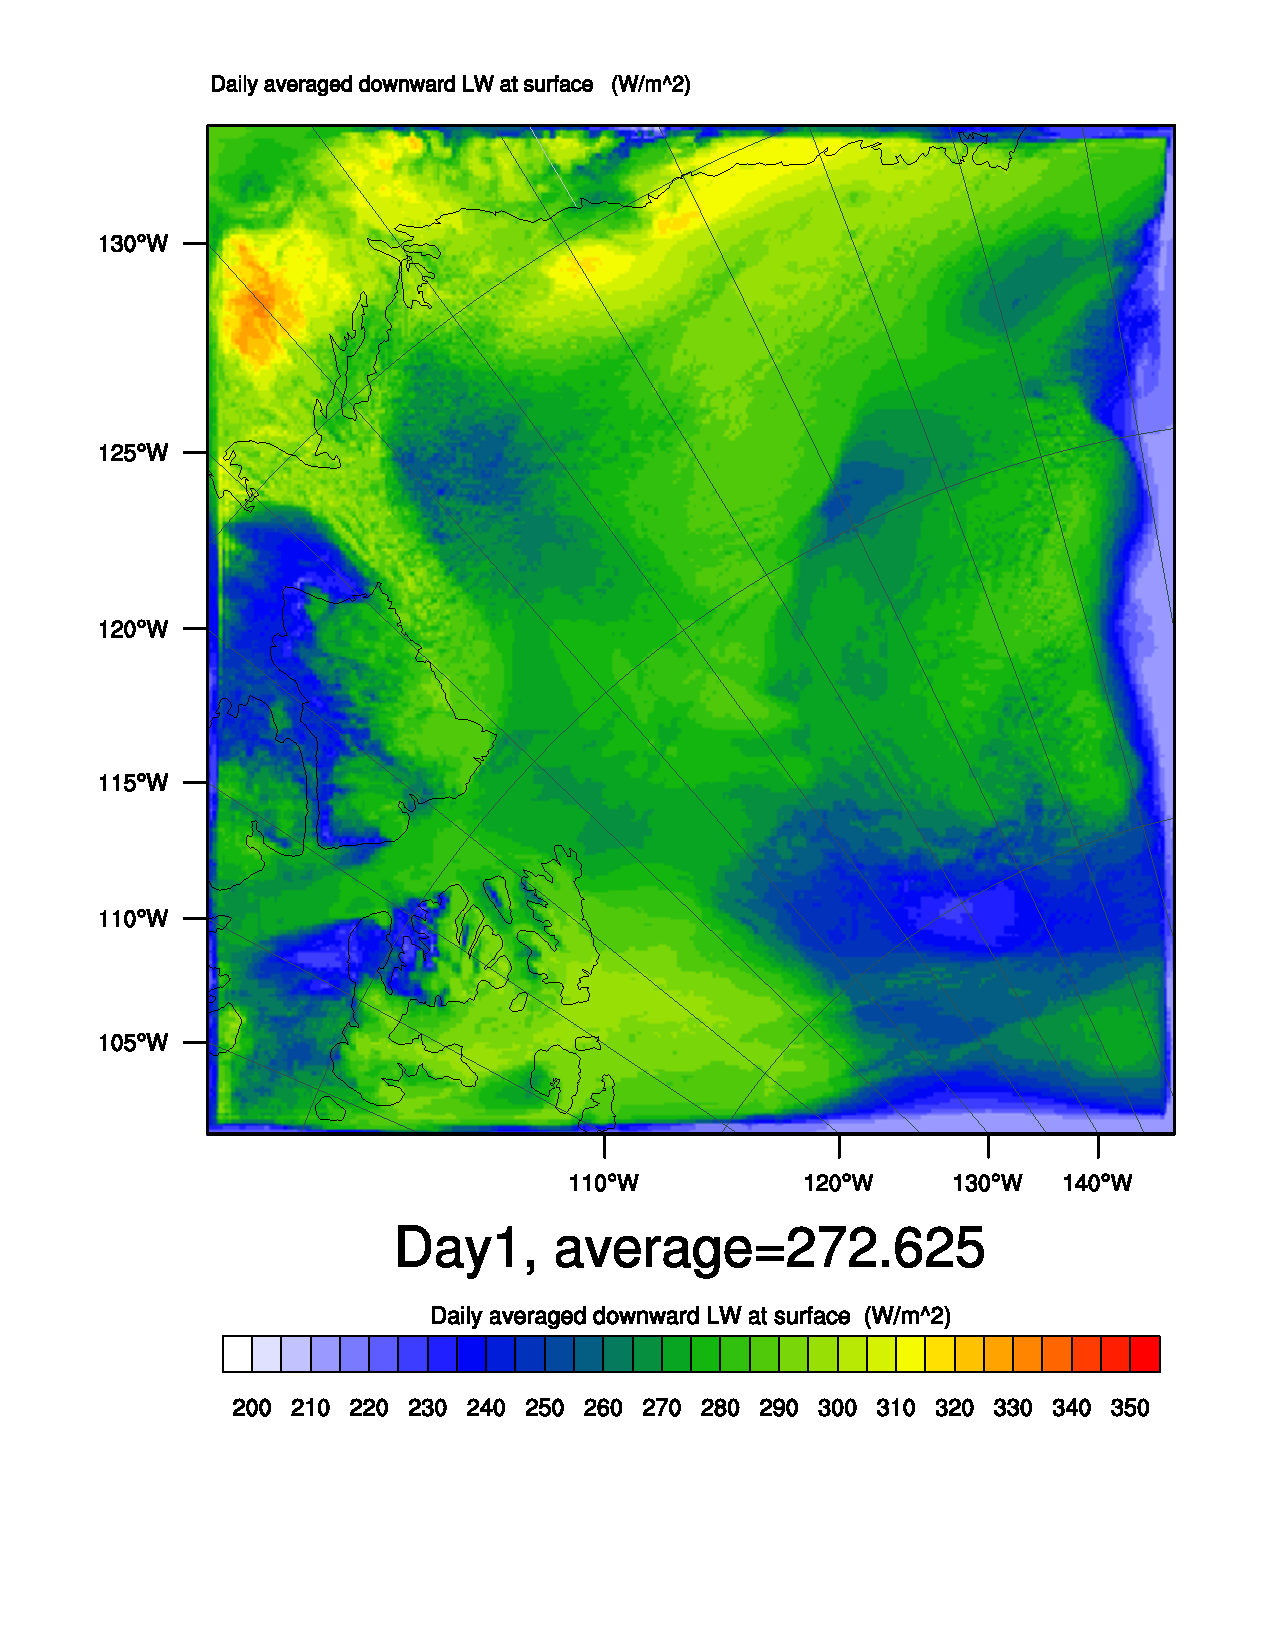
\includegraphics[width=\textwidth]{results/control/GLW_Day1.pdf}
		\caption{LW down at the surface, day 1.}
		\label{subfig:glw_r1Day1}
	\end{subfigure}
	\quad
	\begin{subfigure}{0.48\textwidth}
		\centering
		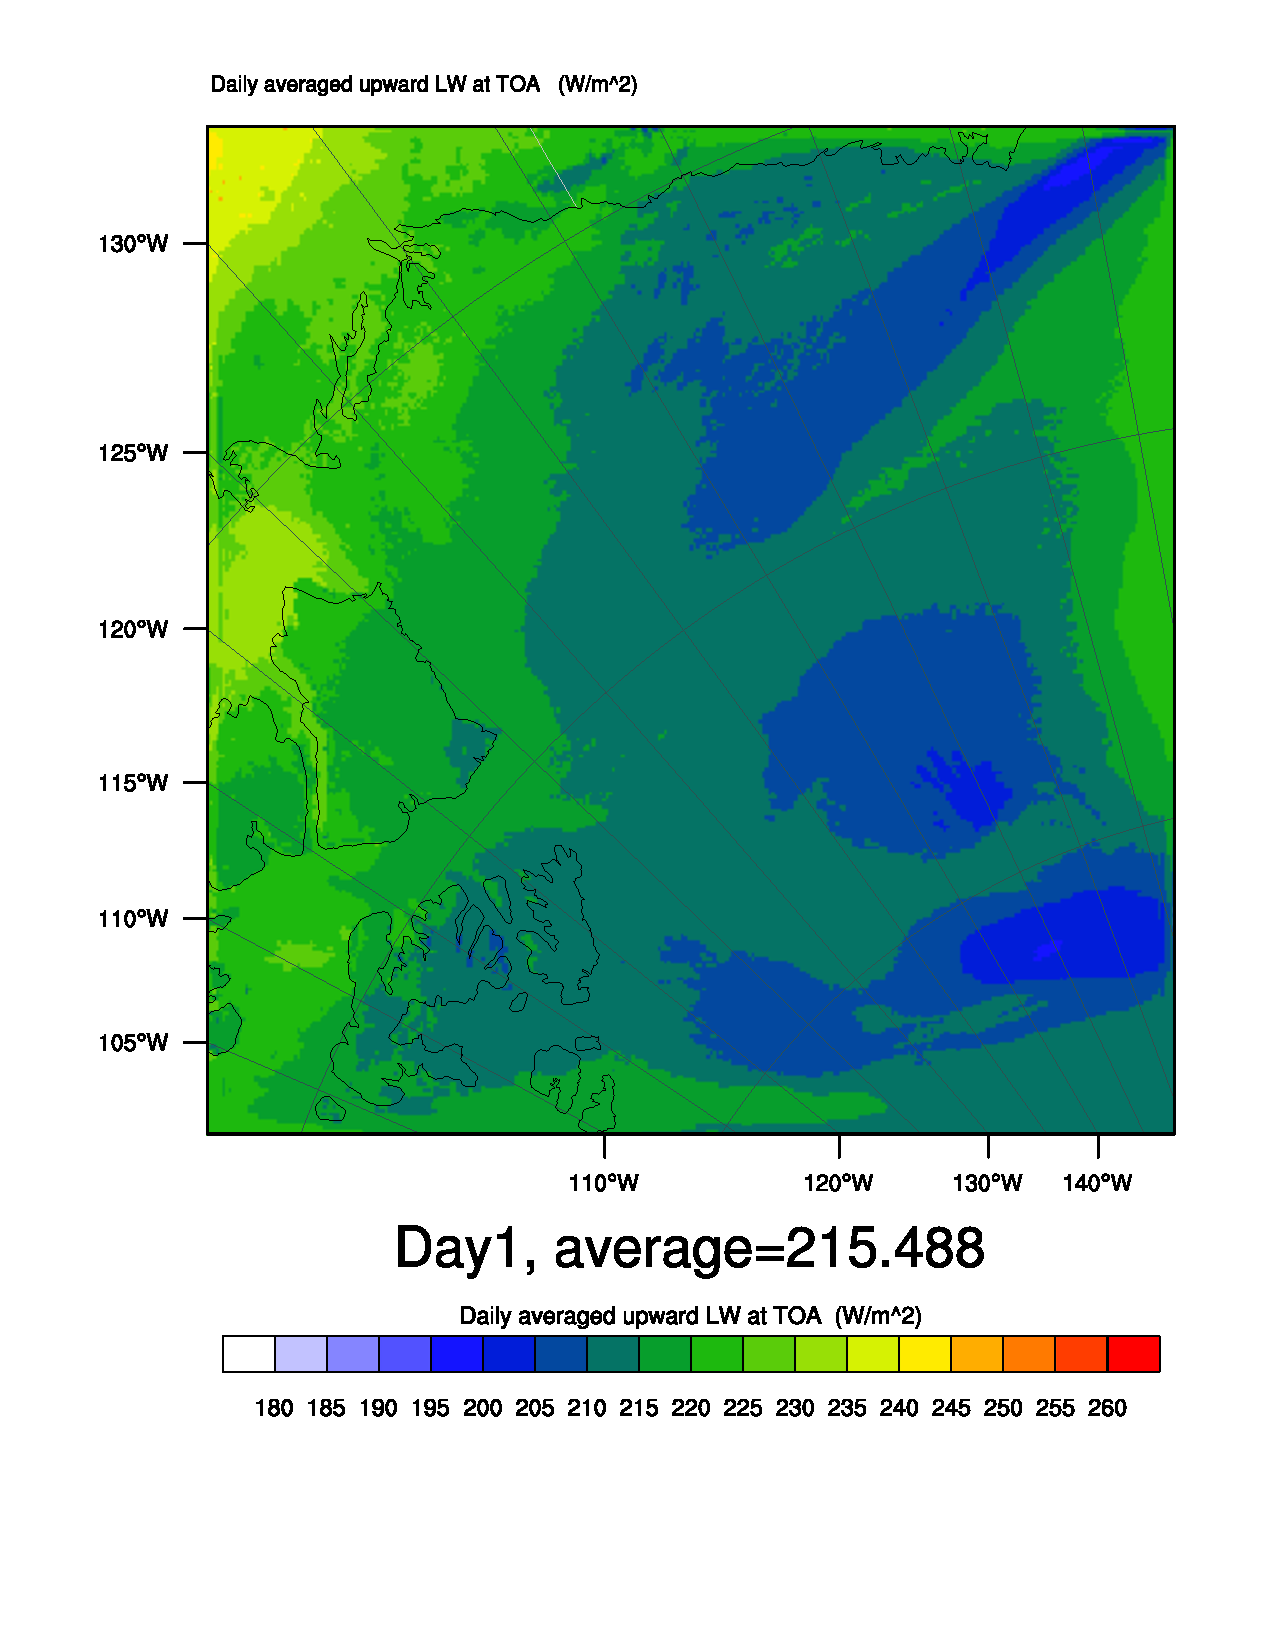
\includegraphics[width=\textwidth]{results/control/LWUPT_Day1.pdf}
		\caption{LW up at TOA, day 1.}
		\label{subfig:lwup_r1Day1}
	\end{subfigure}
	\caption{The average SW and LW flux down at the surface and up at TOA, for day 1. Control.}
	\label{fig:radiation_r1Day1}
\end{figure}

%----- Radiation Day5
\begin{figure}
\centering
	\begin{subfigure}{0.48\textwidth}
		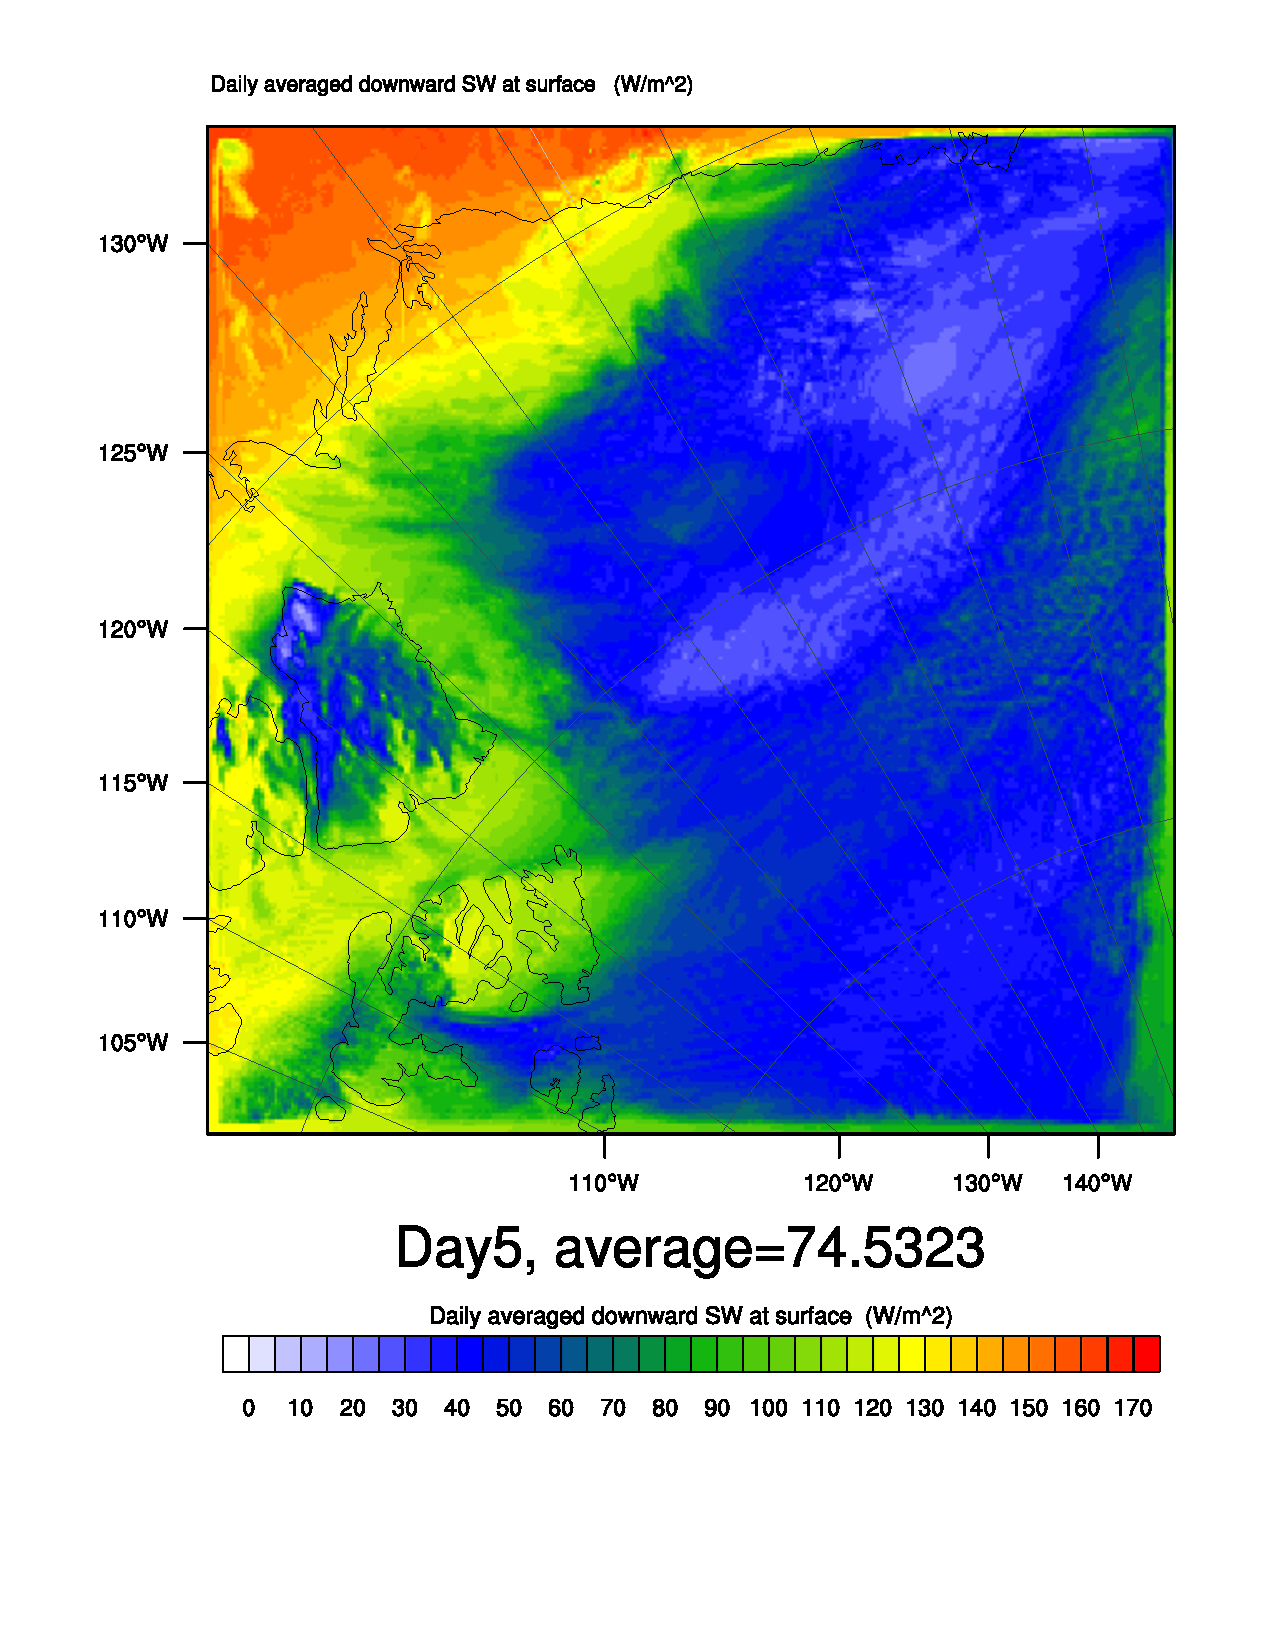
\includegraphics[width=\textwidth]{results/control/SWDOWN_Day5.pdf}
		\caption{The average SW flux down at the surface, day 5.}
		\label{subfig:swdown_r1Day5}
	\end{subfigure}
	\quad
	\begin{subfigure}{0.48\textwidth}
		\centering
		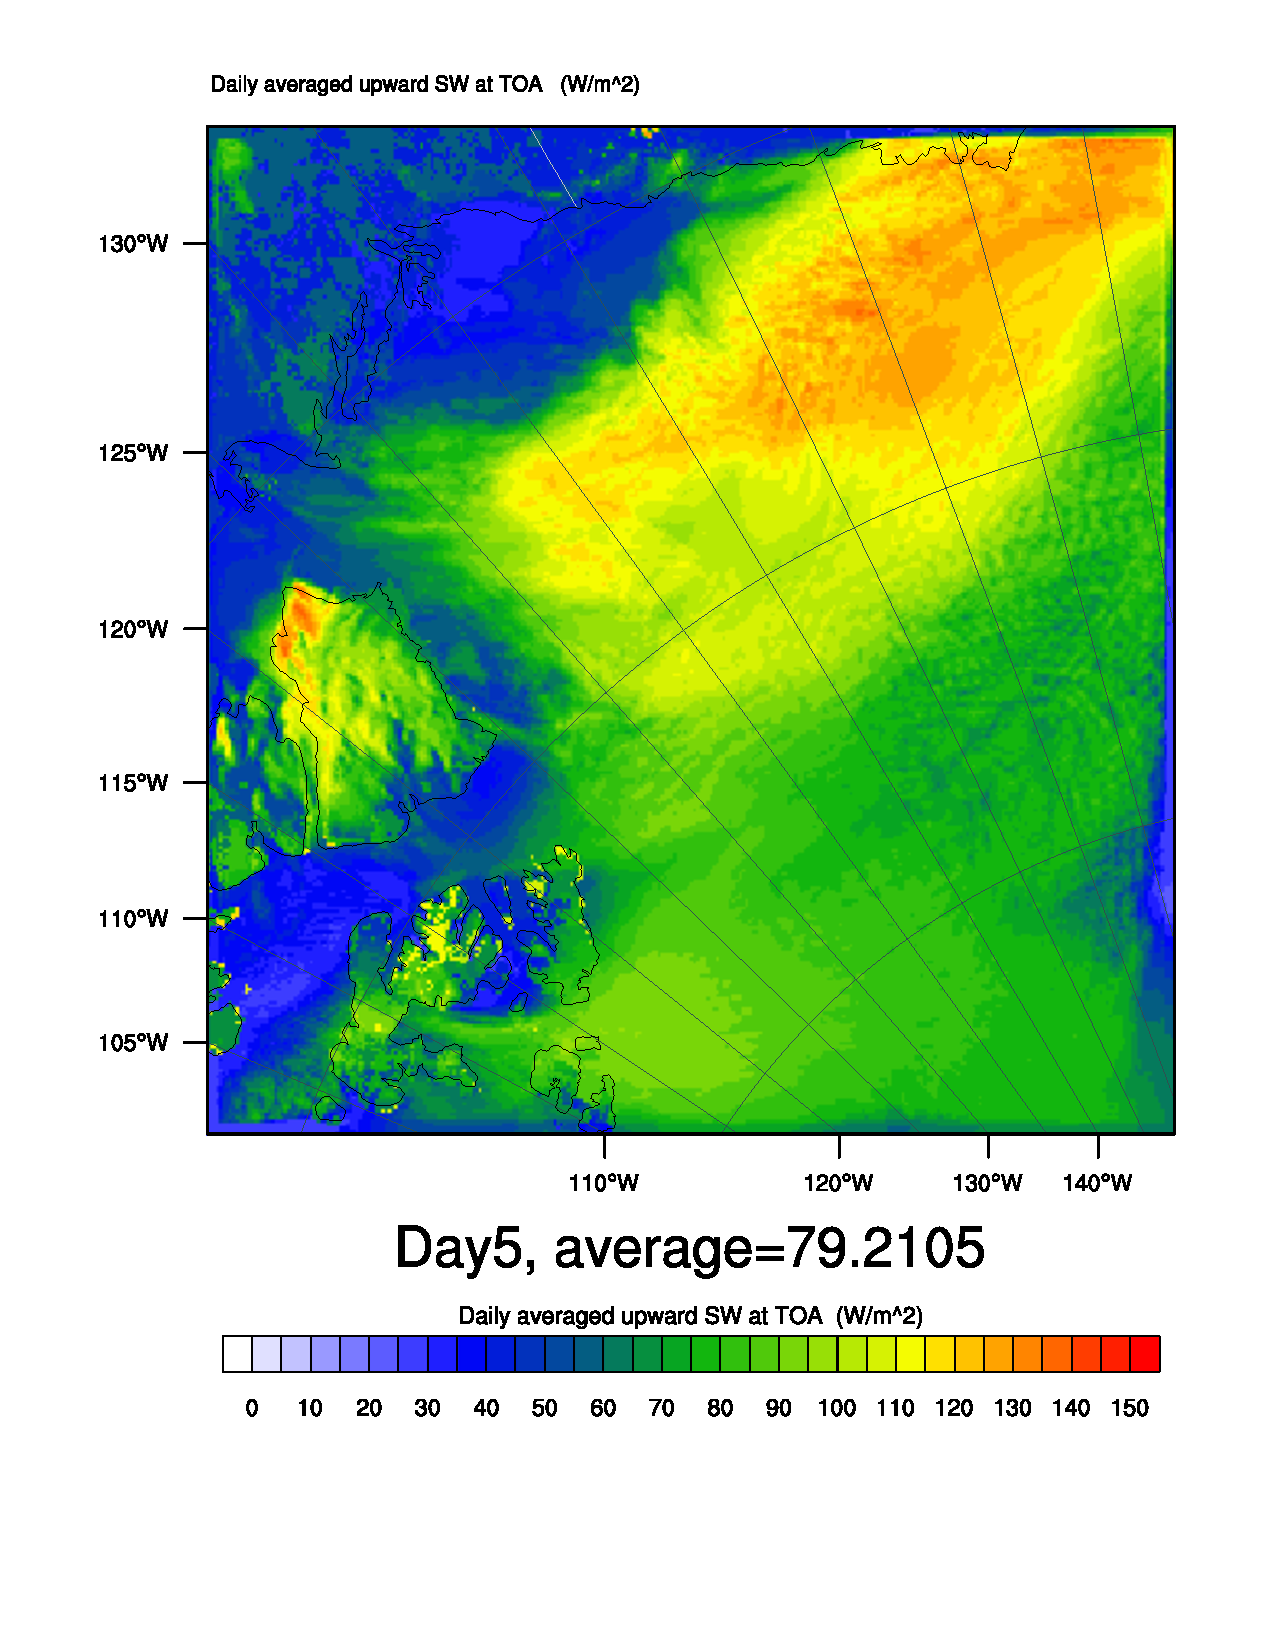
\includegraphics[width=\textwidth]{results/control/SWUPT_Day5.pdf}
		\caption{The average SW flux up at TOA, day 5.}
		\label{subfig:swup_r1Day5}
	\end{subfigure}
	
	\begin{subfigure}{0.48\textwidth}
		\centering
		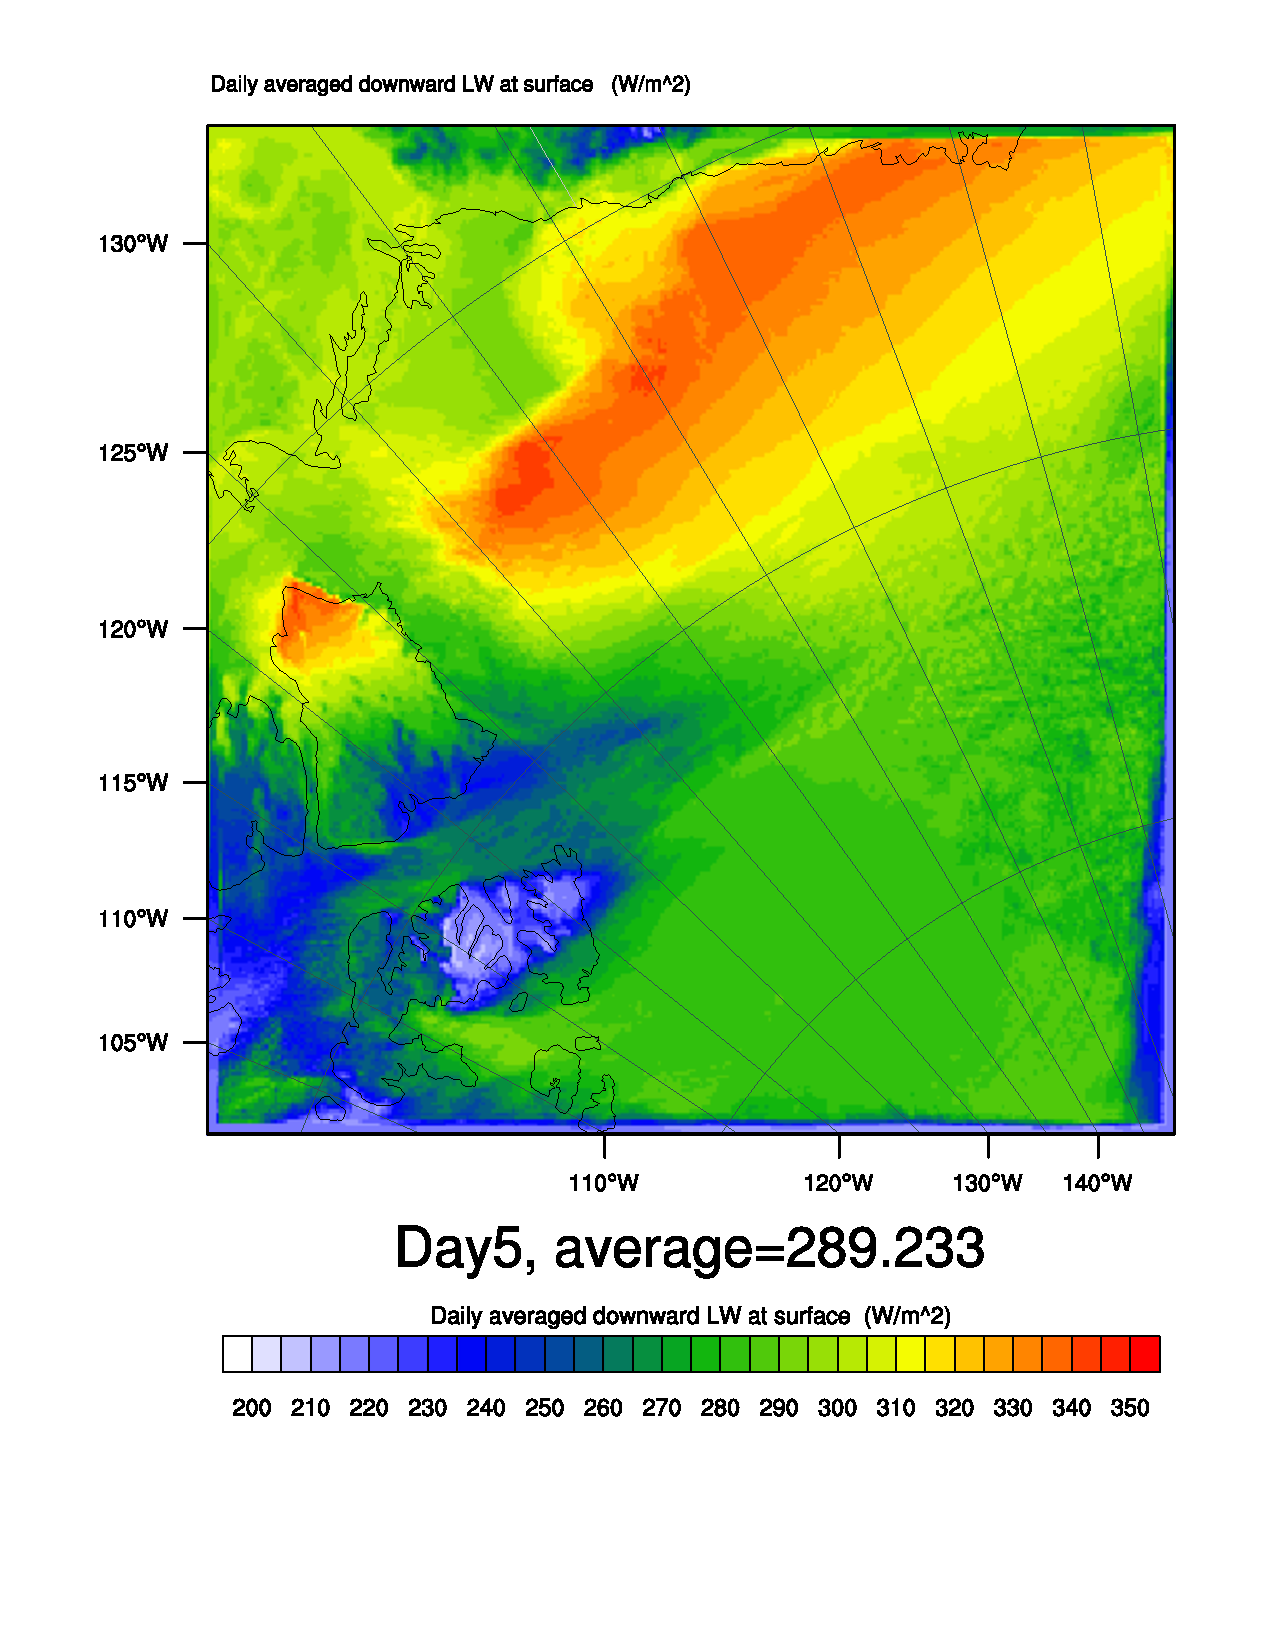
\includegraphics[width=\textwidth]{results/control/GLW_Day5.pdf}
		\caption{The average LW flux down at the surface, day 5.}
		\label{subfig:glw_r1Day5}
	\end{subfigure}
	\quad
	\begin{subfigure}{0.48\textwidth}
		\centering
		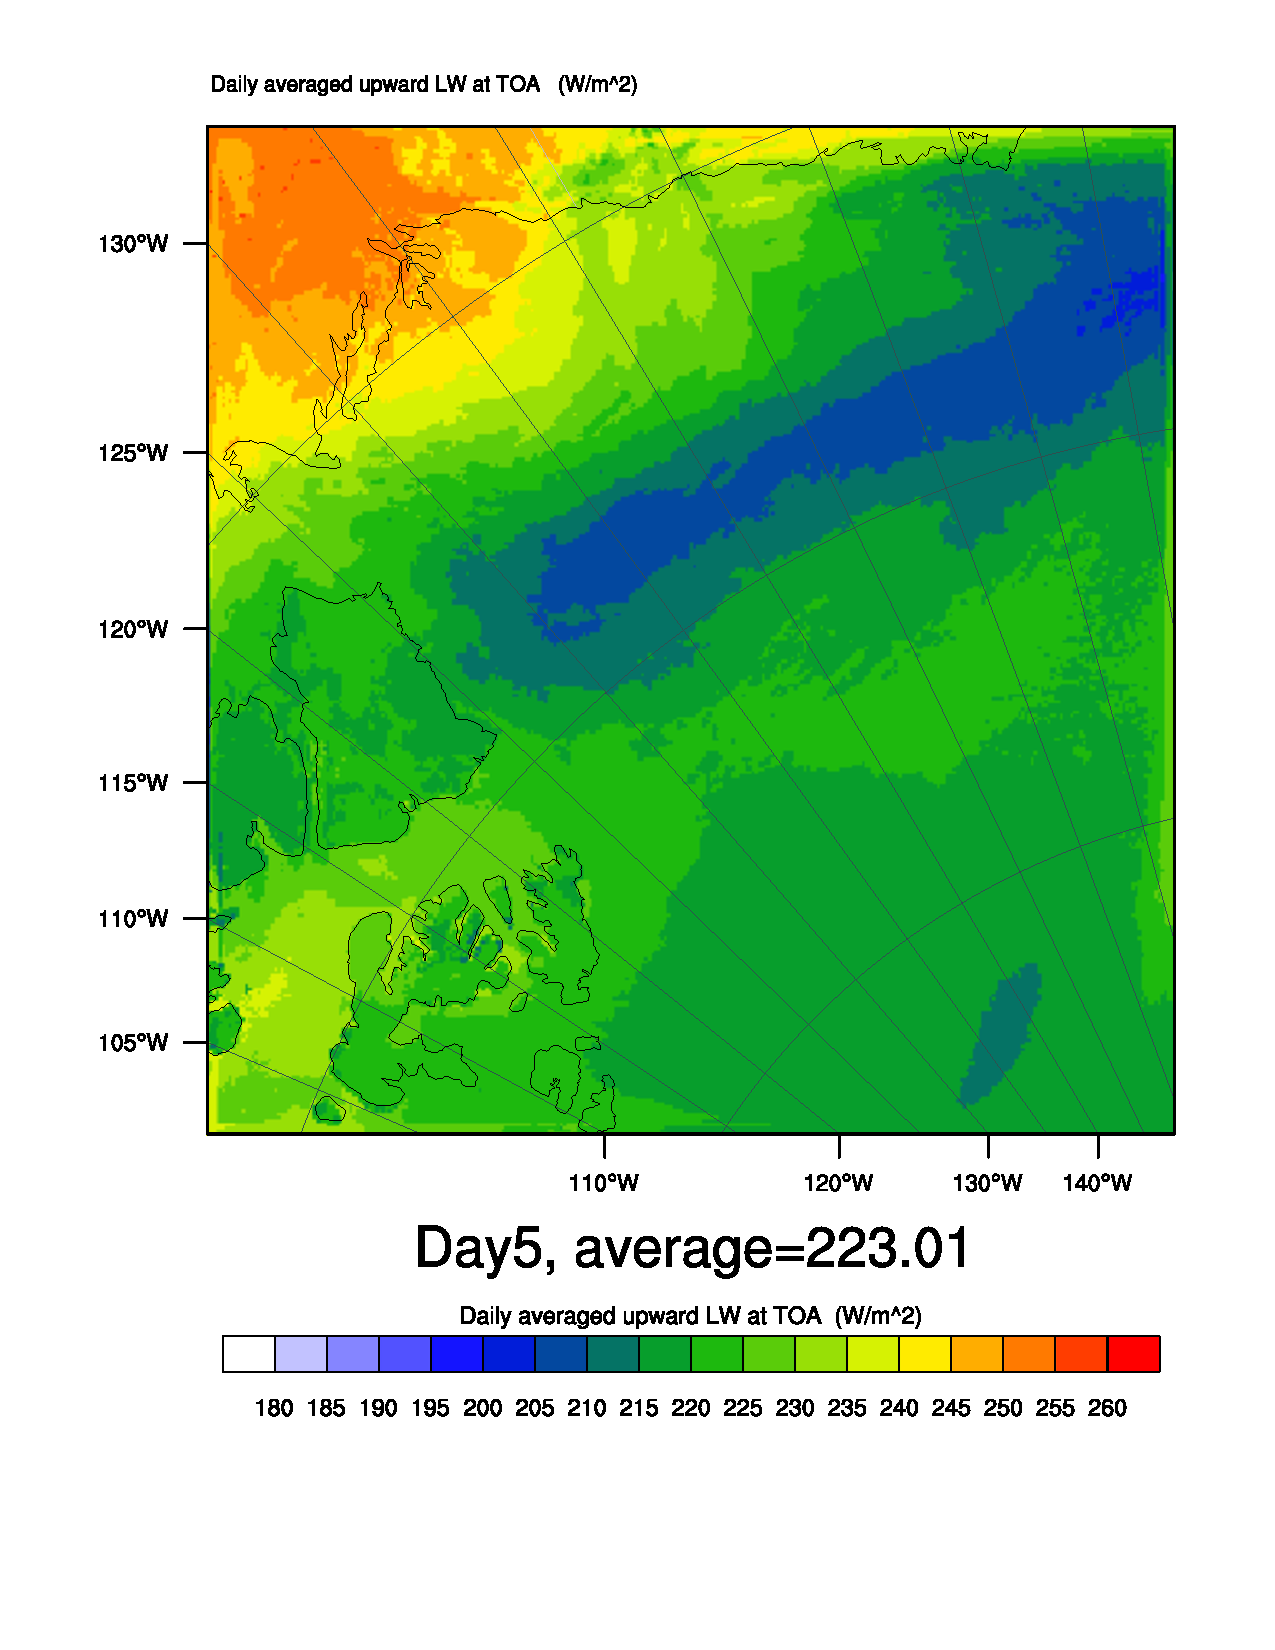
\includegraphics[width=\textwidth]{results/control/LWUPT_Day5.pdf}
		\caption{The average LW flux up at TOA, day 5.}
		\label{subfig:lwup_r1Day5}
	\end{subfigure}
	\caption{The average SW and LW flux down at the surface and up at TOA, for day 5. Control.}
	\label{fig:radiation_r1Day5}
\end{figure}

%----- Surface heat fluxes
\begin{figure}
\centering
	\begin{subfigure}{0.48\textwidth}
		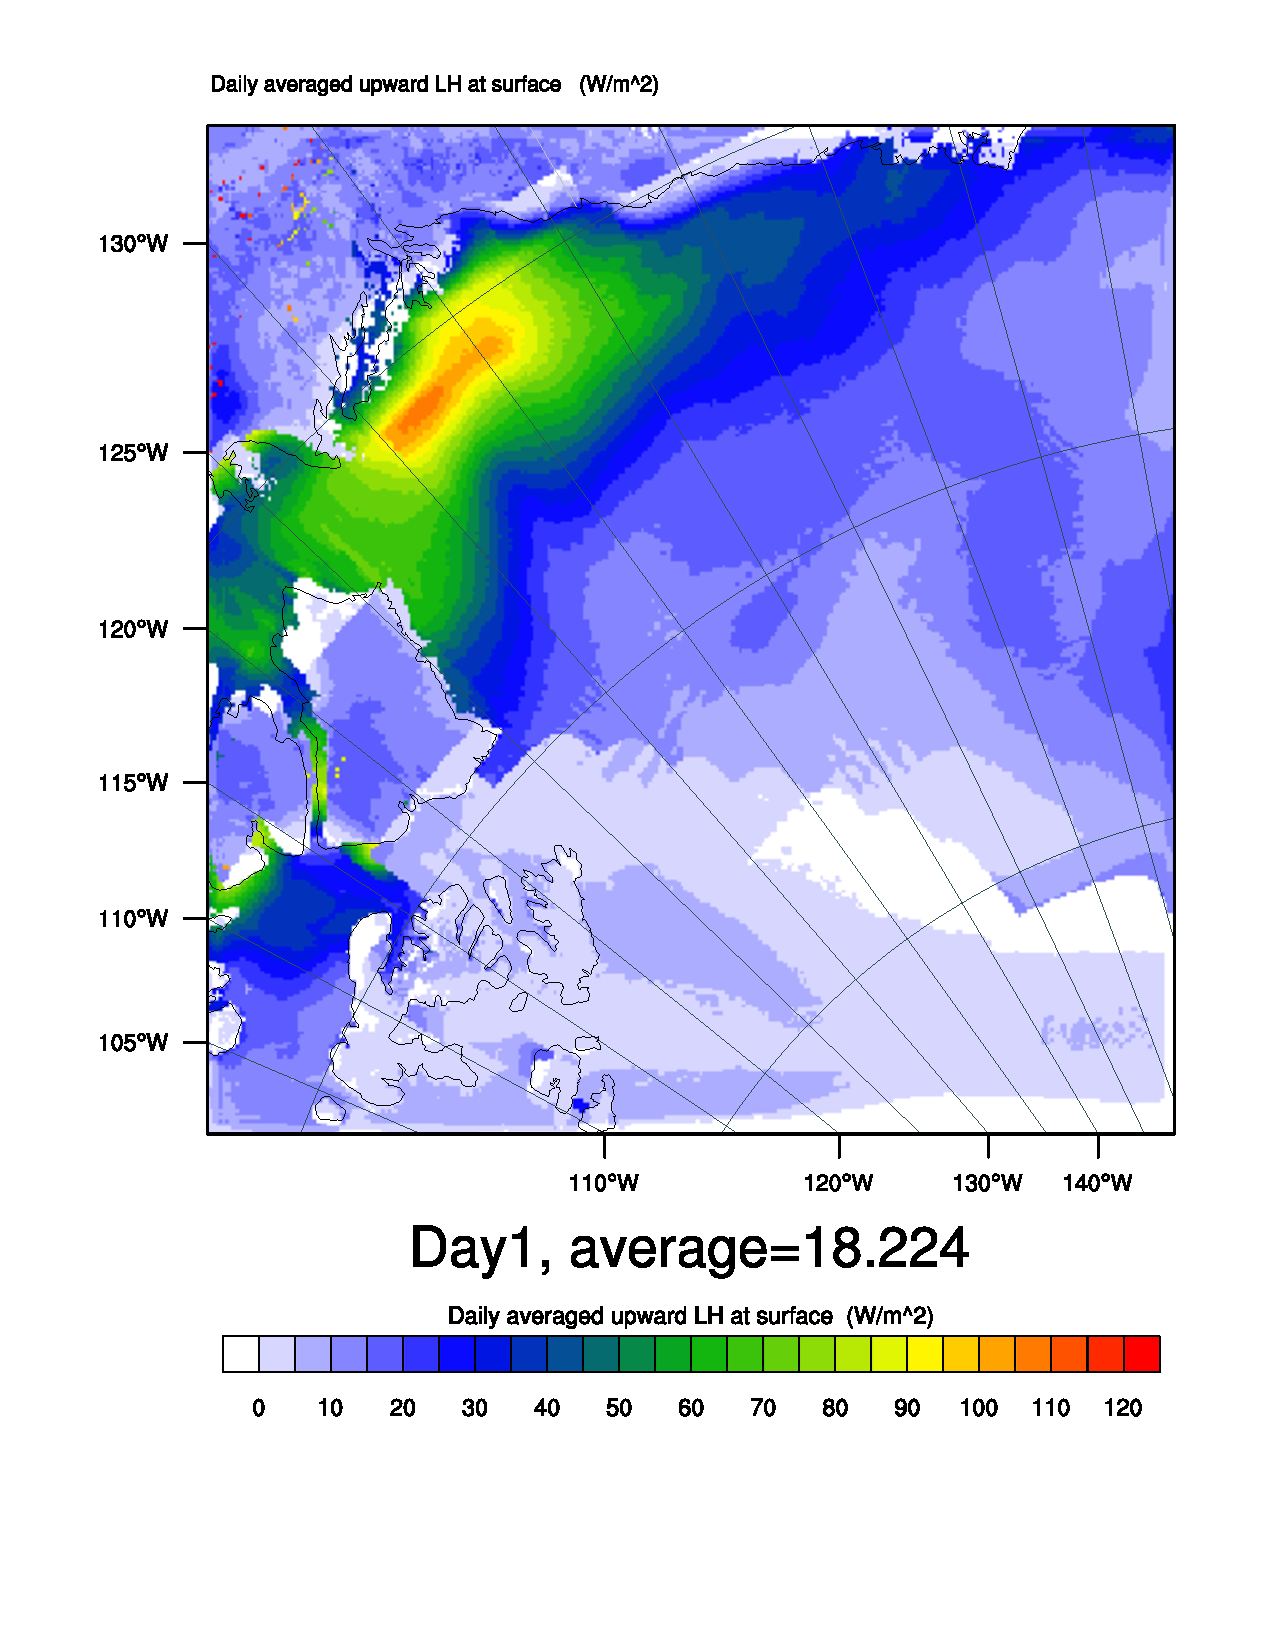
\includegraphics[width=\textwidth]{results/control/LH_Day1.pdf}
		\caption{LH day 1.}
		\label{subfig:lh_r1Day1}
	\end{subfigure}
	\quad
	\begin{subfigure}{0.48\textwidth}
		\centering
		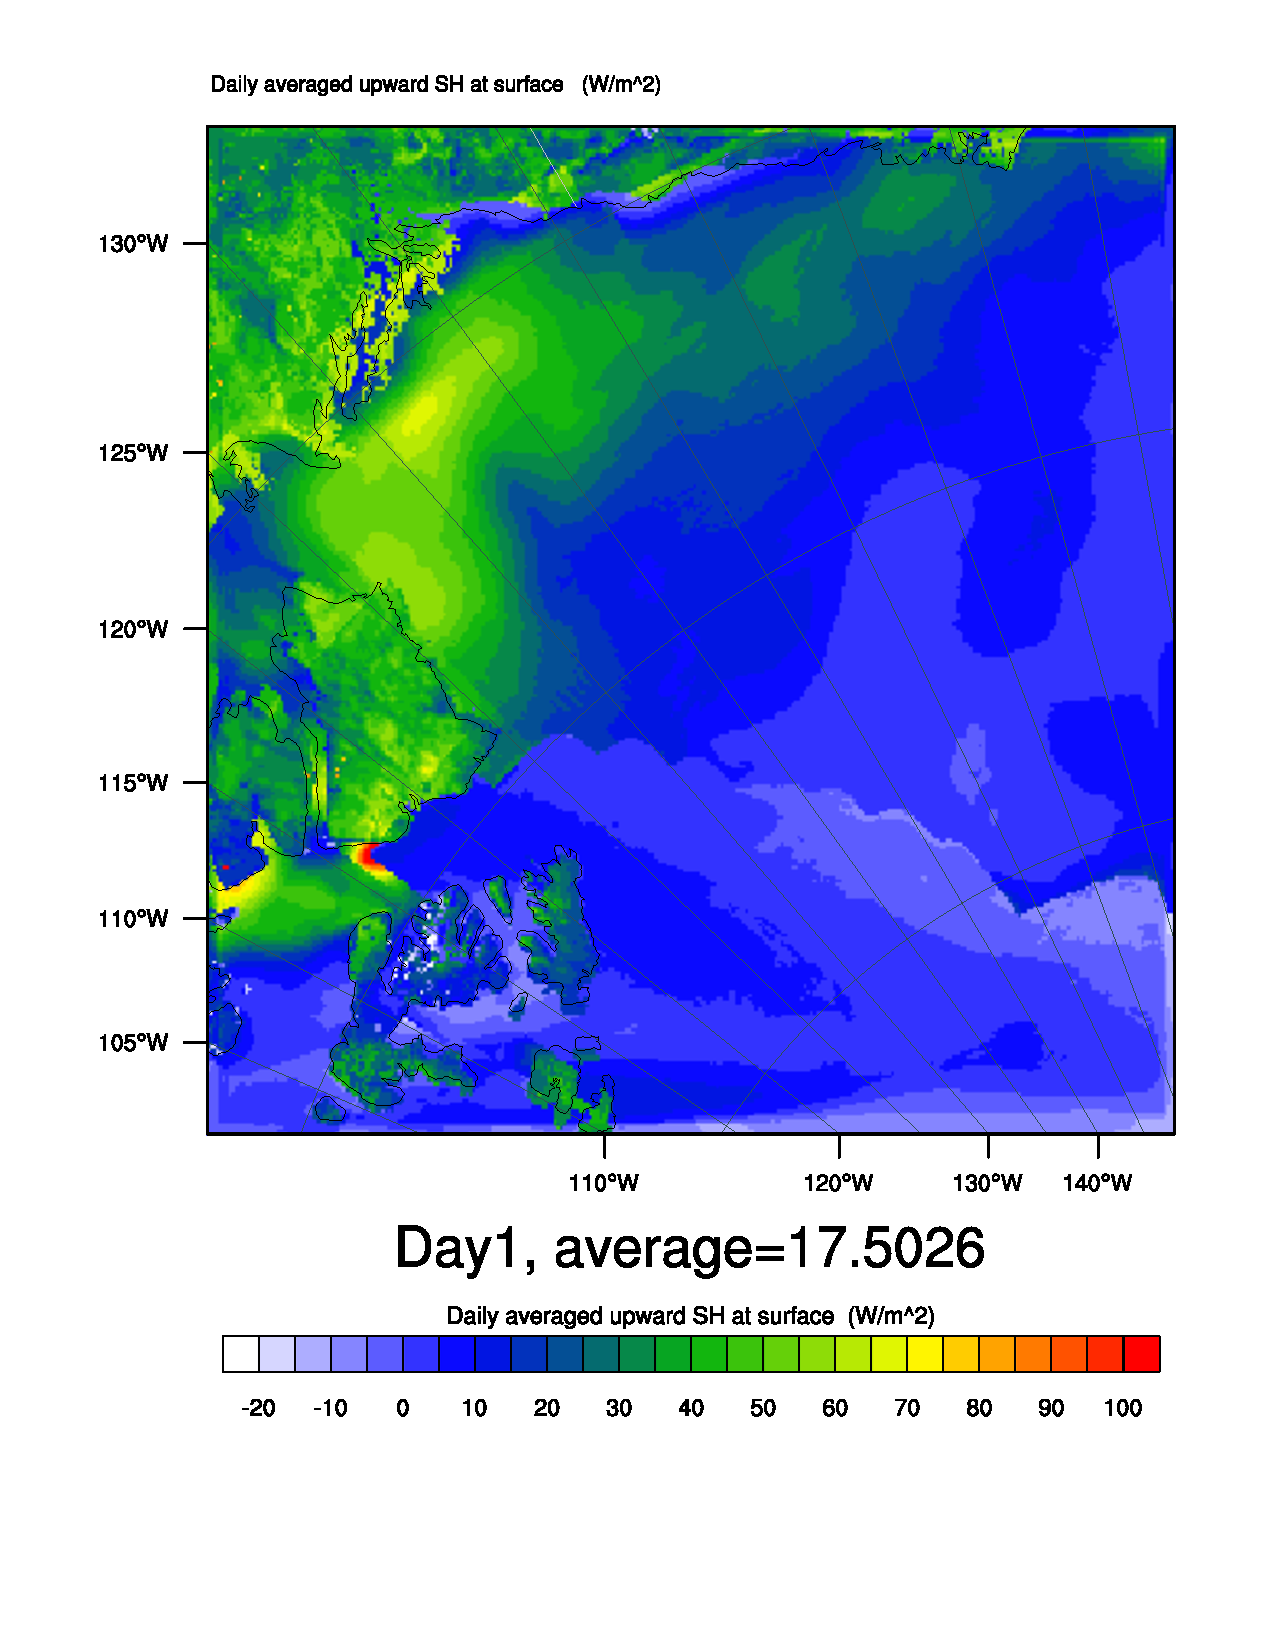
\includegraphics[width=\textwidth]{results/control/HFX_Day1.pdf}
		\caption{SH day 1.}
		\label{subfig:sh_r1Day1}
	\end{subfigure}
	
	\begin{subfigure}{0.48\textwidth}
		\centering
		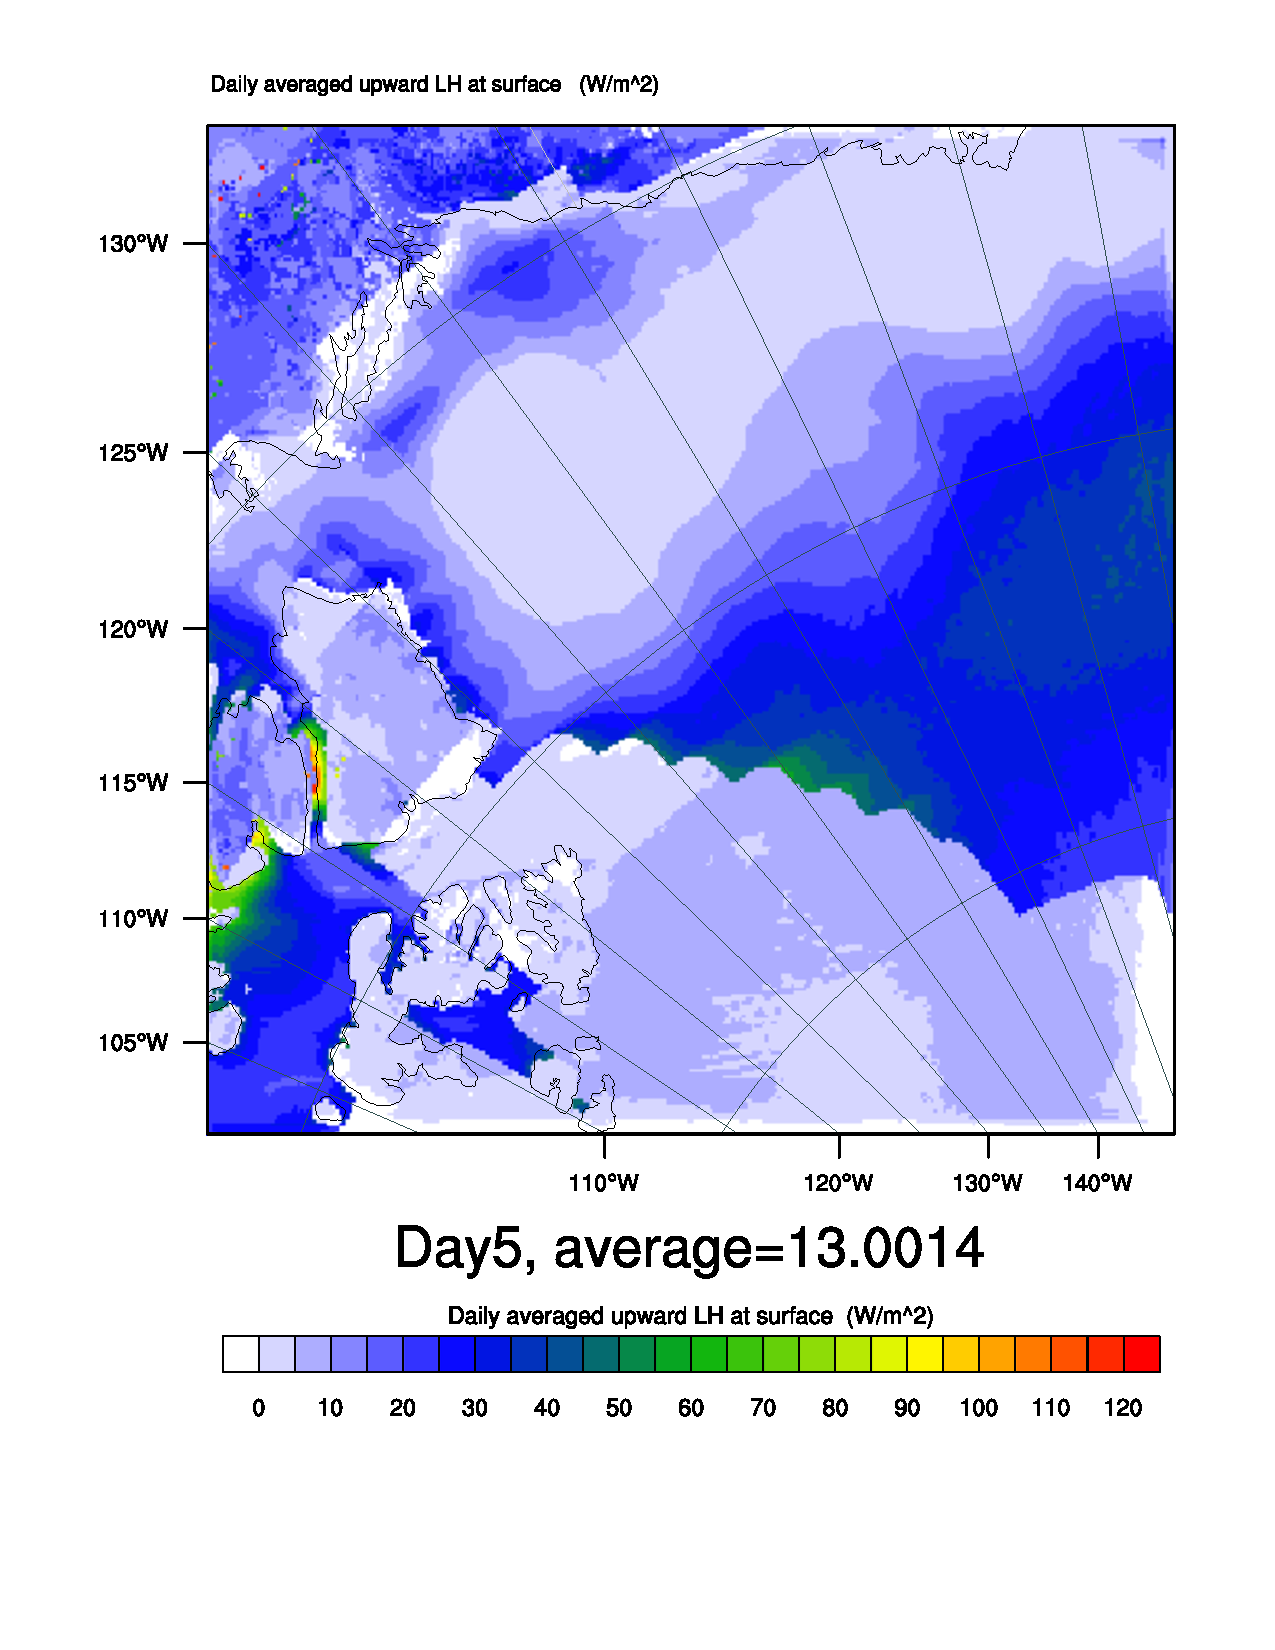
\includegraphics[width=\textwidth]{results/control/LH_Day5.pdf}
		\caption{LH day 5.}
		\label{subfig:lh_r1Day5}
	\end{subfigure}
	\quad
	\begin{subfigure}{0.48\textwidth}
		\centering
		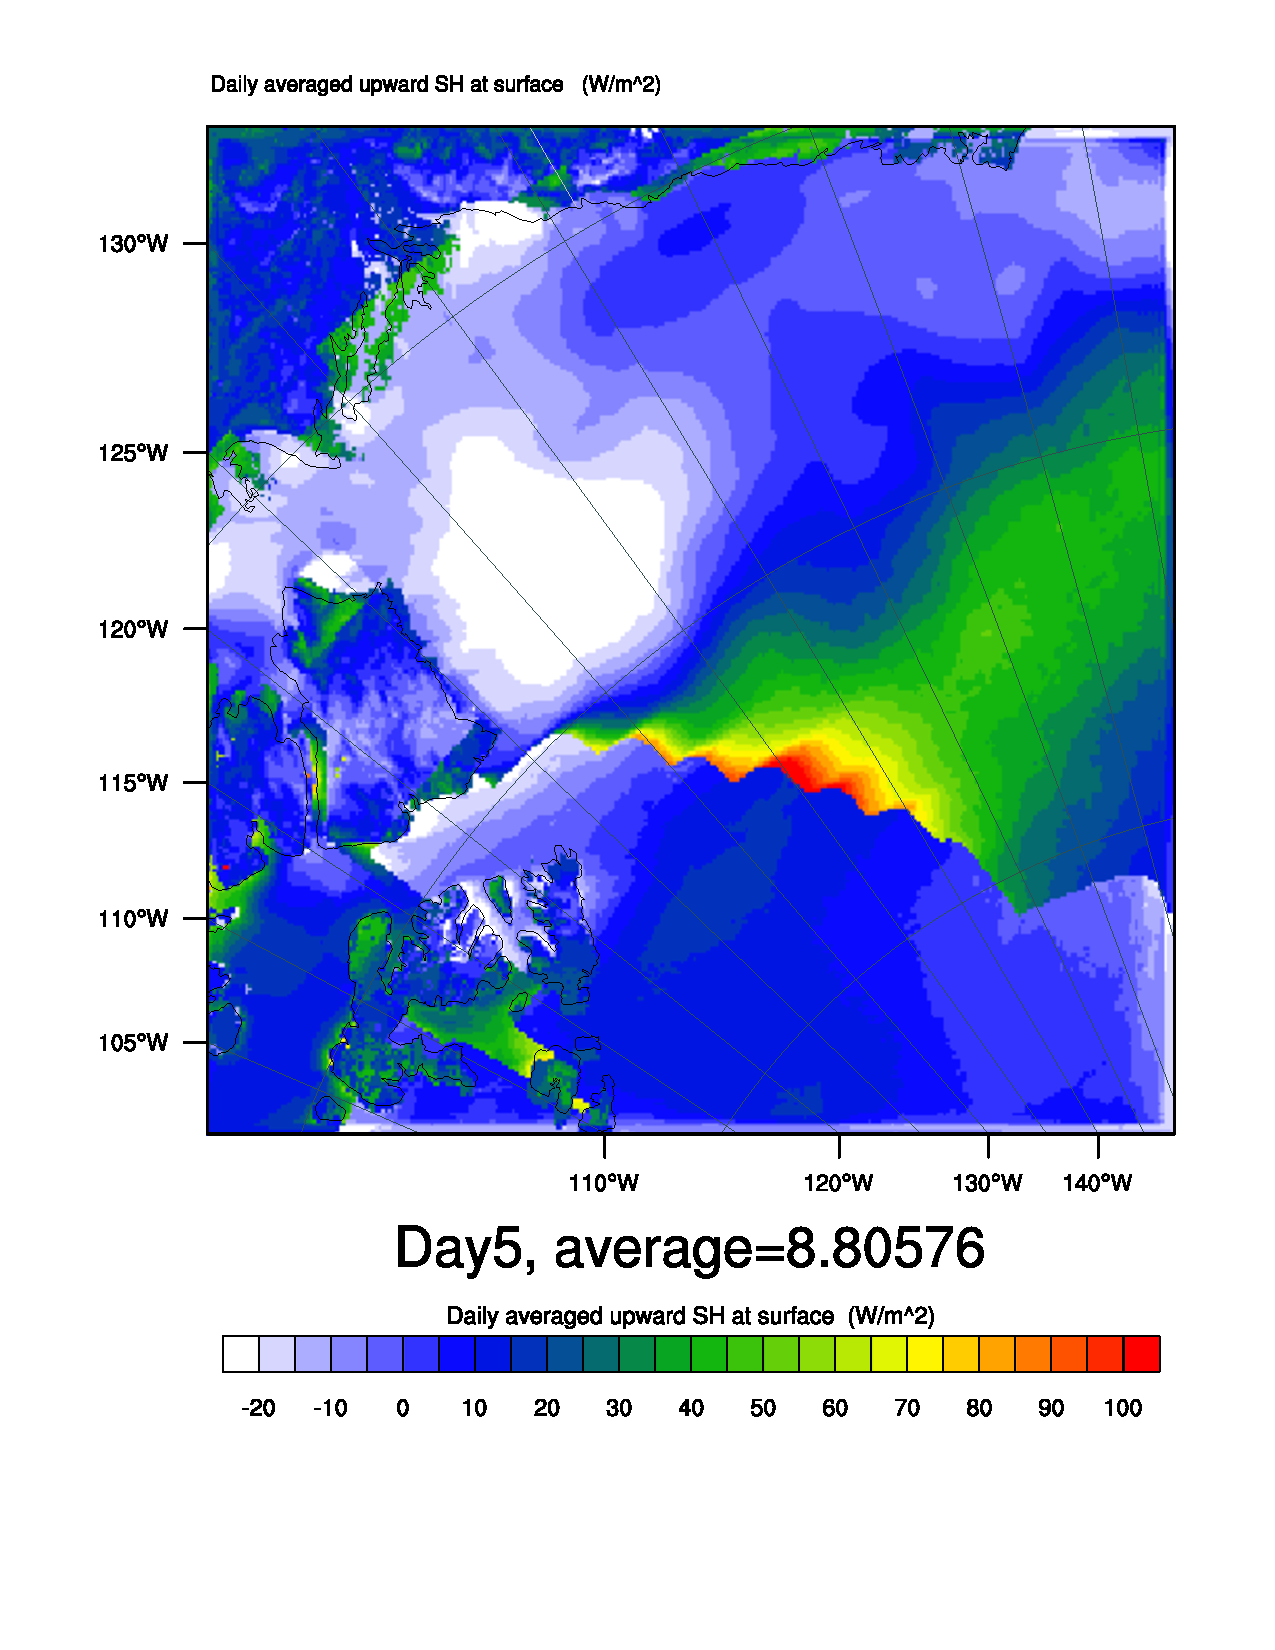
\includegraphics[width=\textwidth]{results/control/HFX_Day5.pdf}
		\caption{SH day 5.}
		\label{subfig:sh_r1Day5}
	\end{subfigure}
	\caption{The average surface heat fluxes (SH and LH) up at the surface, for days 1 and 5. Control.}
	\label{fig:surface_fluxes_r1}
\end{figure}

%--------- Cloud ice number concentration
\begin{figure}
	\begin{subfigure}{0.48\textwidth}
		\centering
		\includegraphics[width=\textwidth]{results/control/QNICE_day1.pdf}
		\caption{CINC day 1}
		\label{subfig:cinc_cont_Day1}
	\end{subfigure}
	\begin{subfigure}{0.48\textwidth}
		\centering
		\includegraphics[width=\textwidth]{results/control/QNICE_day5.pdf}
		\caption{CINC day 5}
		\label{subfig:cinc_cont_Day5}
	\end{subfigure}
	\caption{Cloud ice number concentration (CINC), plotted over the area, averaged over the lower 11 layers and days 1 and 5. Control.}
	\label{fig:cloudice}
\end{figure}

%-------------------------------
\clearpage
\section{Removed sea ice}
%-------------------------------
The sea ice was removed to study the effect this had on 
 that was there in the control run, but has been removed for NoIce, is shown in figure~\ref{fig:seaice}. @\textit{Explain why sea ice was removed, repeat stuff from earlier!}

\begin{figure}[hb]
\centering
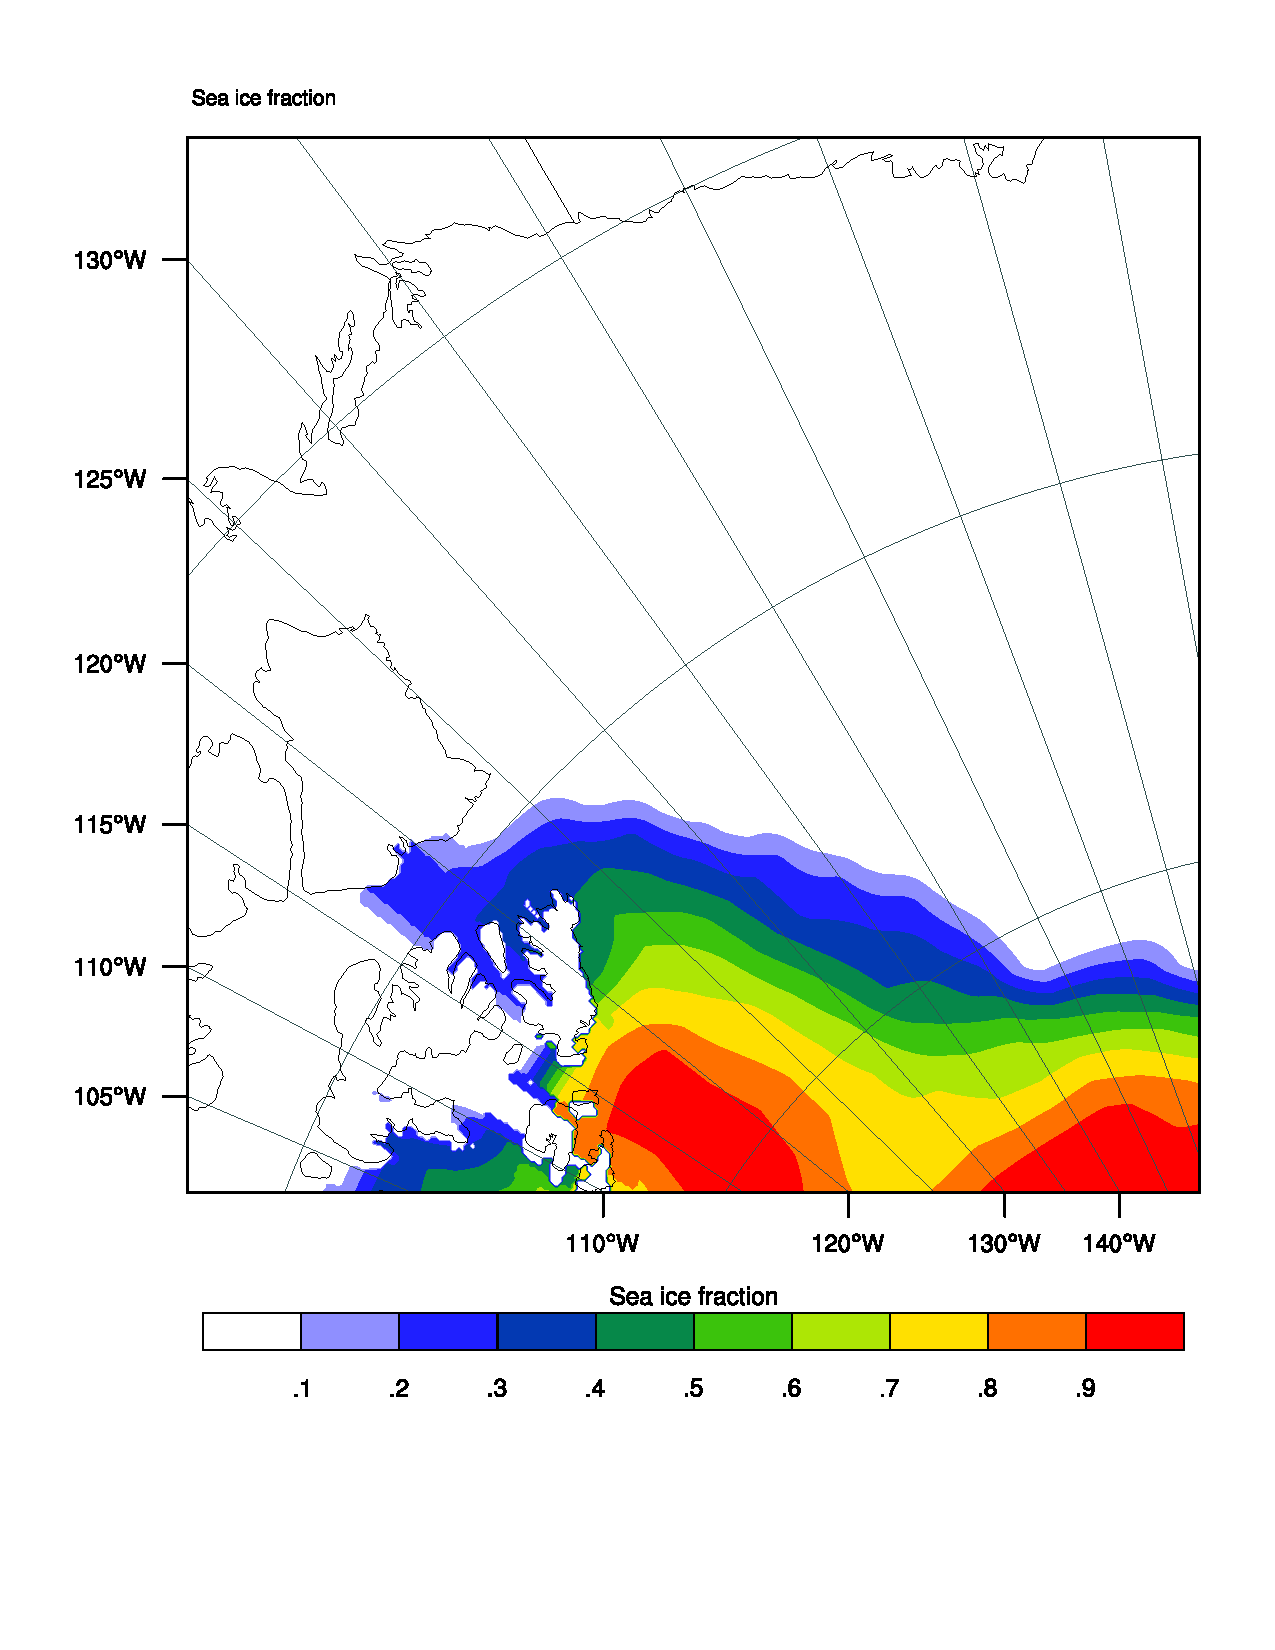
\includegraphics[width=0.5\textwidth]{results/control/seaiceplot.pdf}
\caption{Sea ice fraction in Control (and Aero10).}
\label{fig:seaice}
\end{figure}

\subsection{Day 1}
\label{sec:noiceDay1}
The average difference in LWP, NoIce-Control, for day 1, shown in figure~\ref{subfig:LWPr2Day1} is small (@??) for the whole field ($\sim$0.23$\text{g/m}^2$ increase). But the area of interest in this case is where the sea ice is not present, which it was in the control run (figure~\ref{fig:seaice}). The sea ice edge is also included as a black contour in figure~\ref{subfig:cross_line}. The area where there was sea ice in the control run shows a positive difference in LWP. Especially furthest north (bottom right corner of the map) the LWP is significantly higher, >15$\text{g/m}^2$.

\begin{figure}
\centering
	\begin{subfigure}{0.30\textwidth}
		\centering
		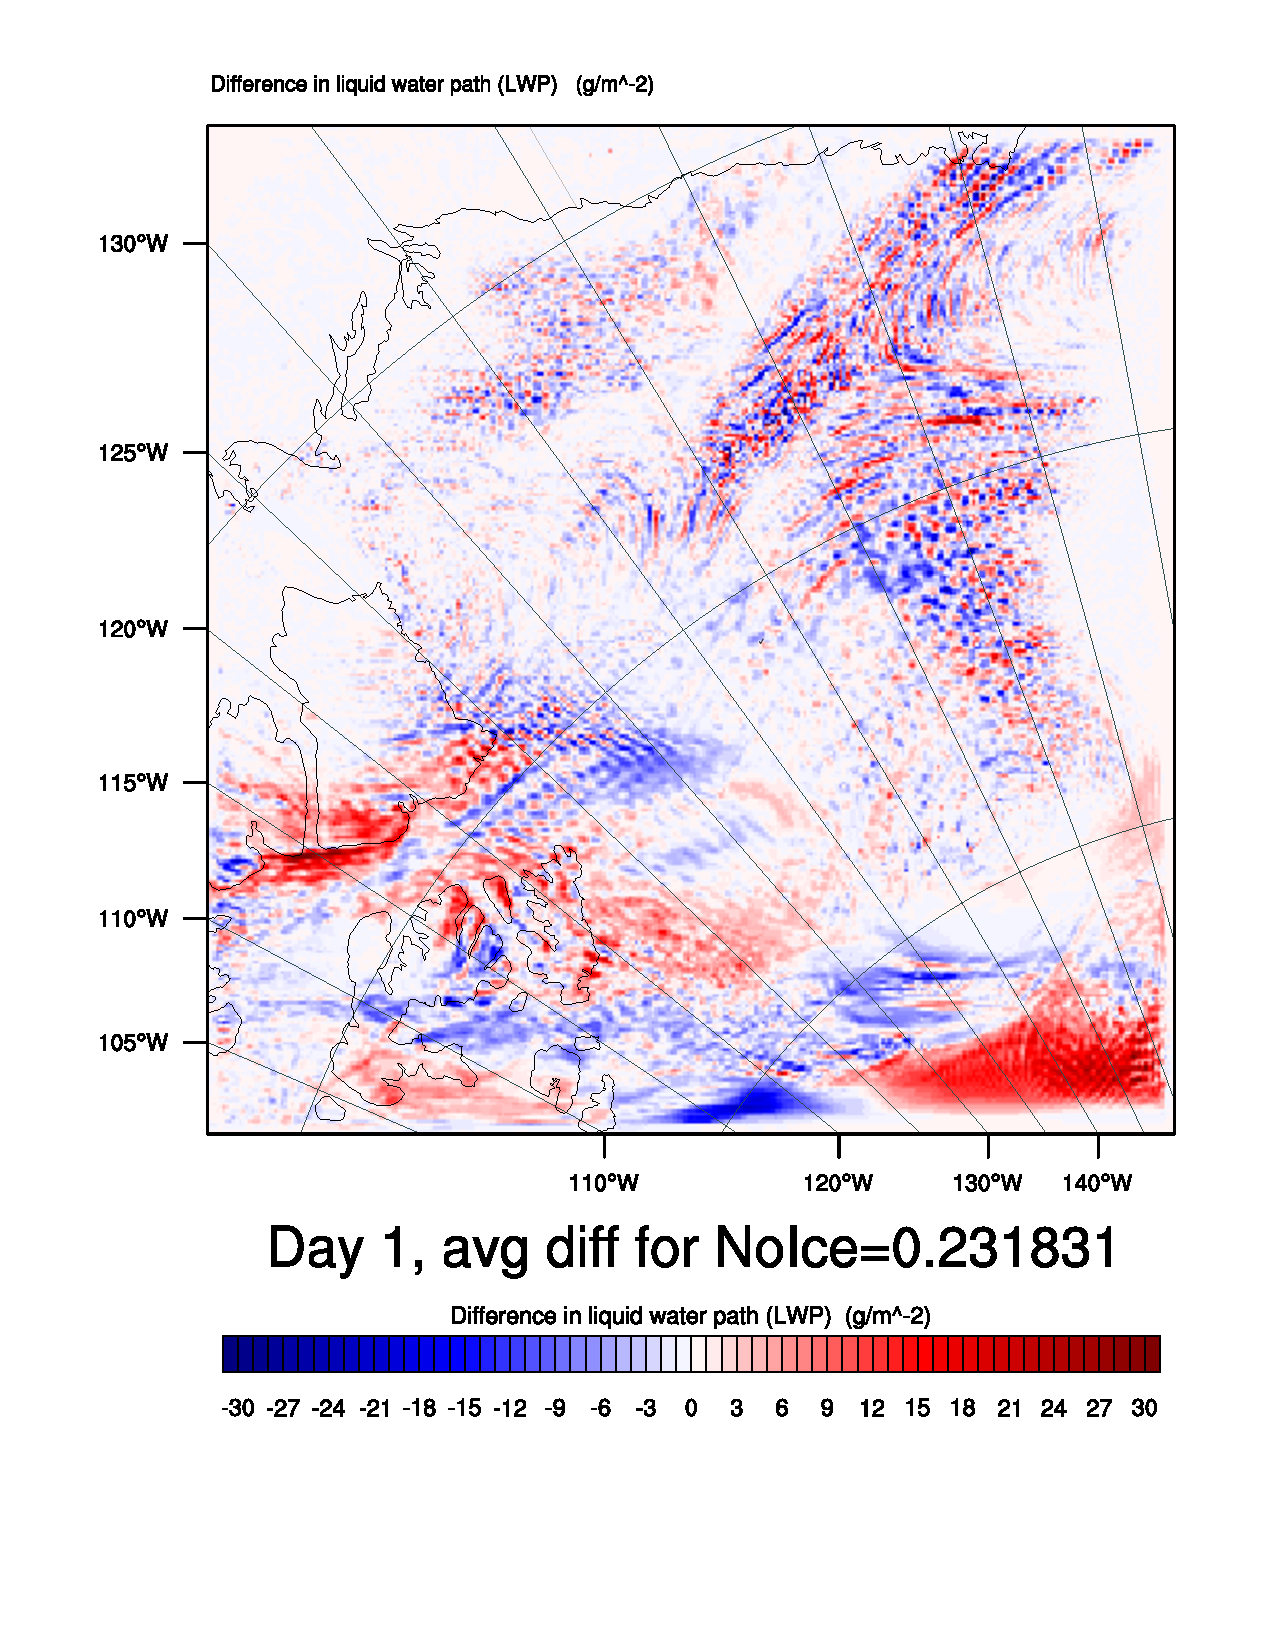
\includegraphics[width=\textwidth]{results/noice/Diff_LWP_Day1NoIce.pdf}
		\caption{LWP, NoIce, day 1}
		\label{subfig:LWPr2Day1}
	\end{subfigure}
	\begin{subfigure}{0.30\textwidth}
		\centering
		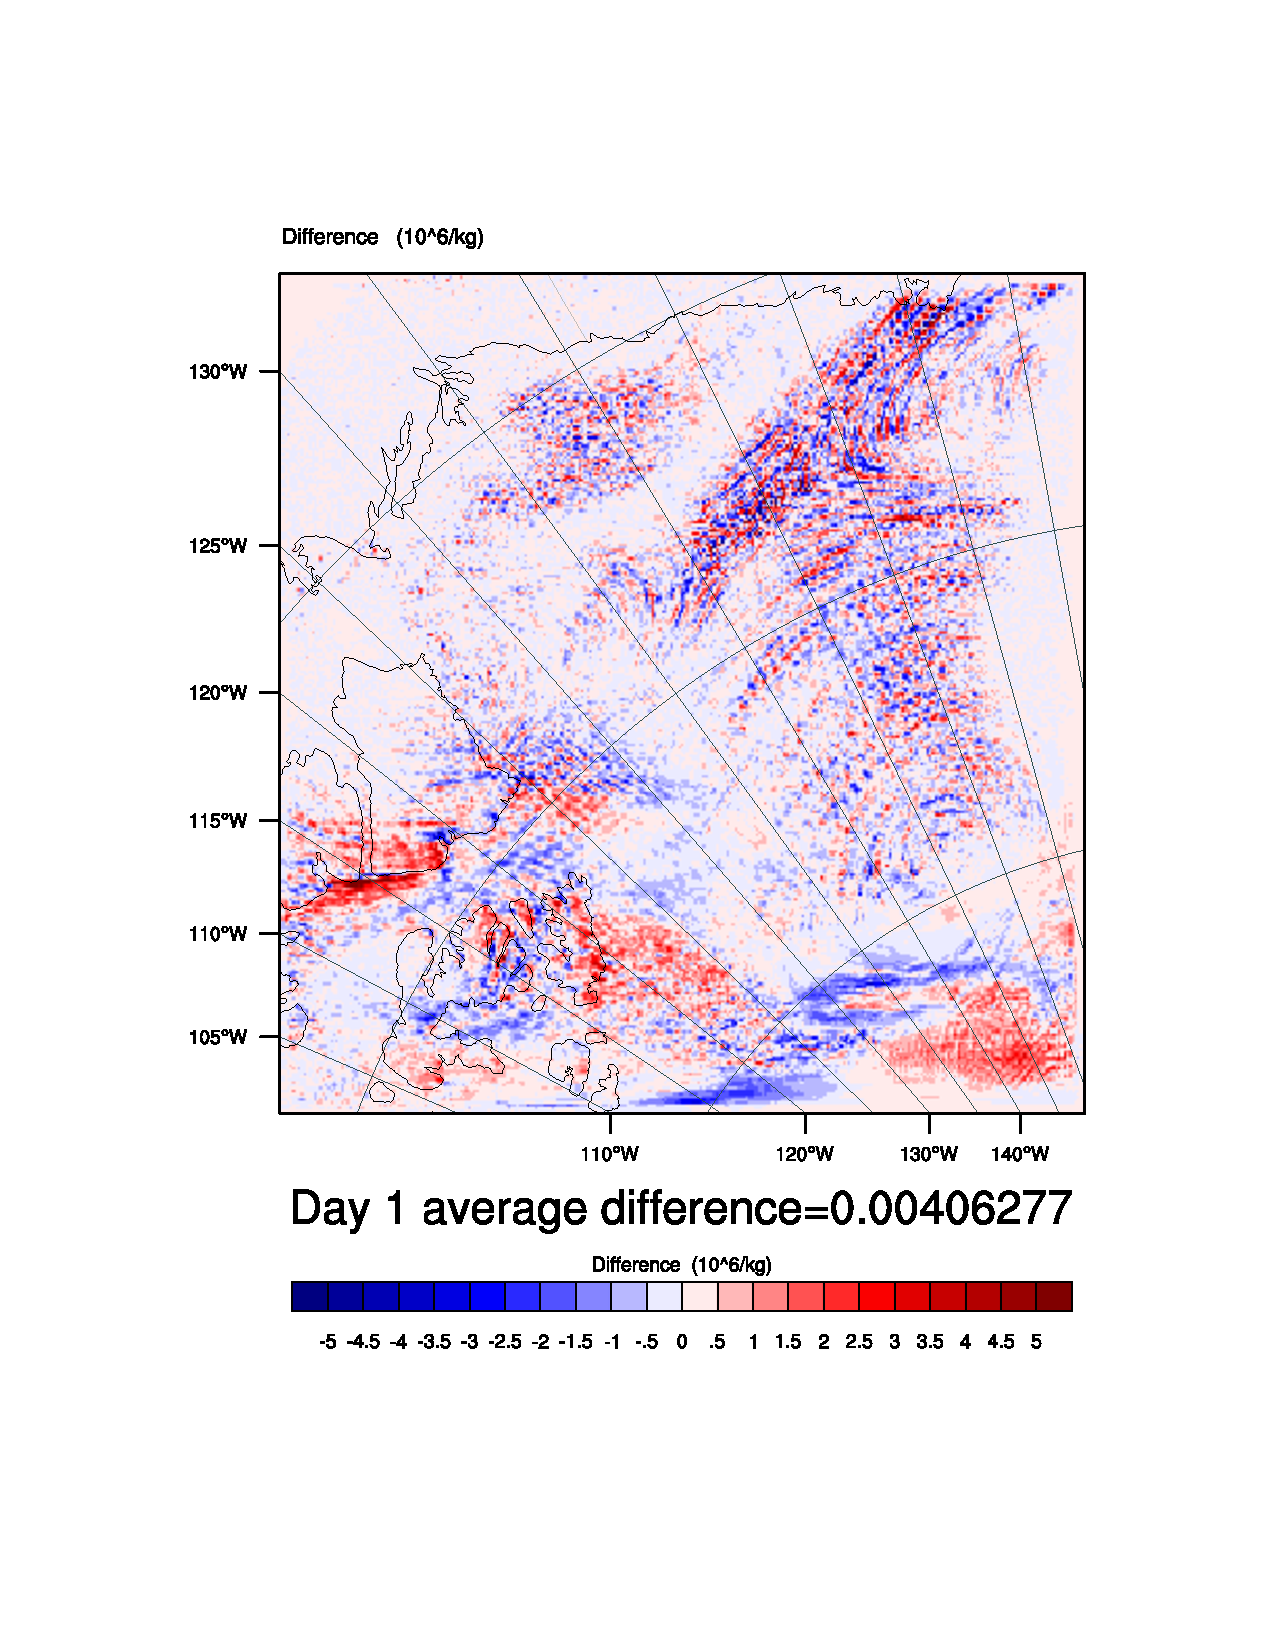
\includegraphics[width=\textwidth]{results/noice/diff_NoIce_QNCLOUD_Day1.pdf}
		\caption{CDNC, NoIce, day 1}
		\label{subfig:CDNCr2Day1}
	\end{subfigure}
	\begin{subfigure}{0.30\textwidth}
		\centering
		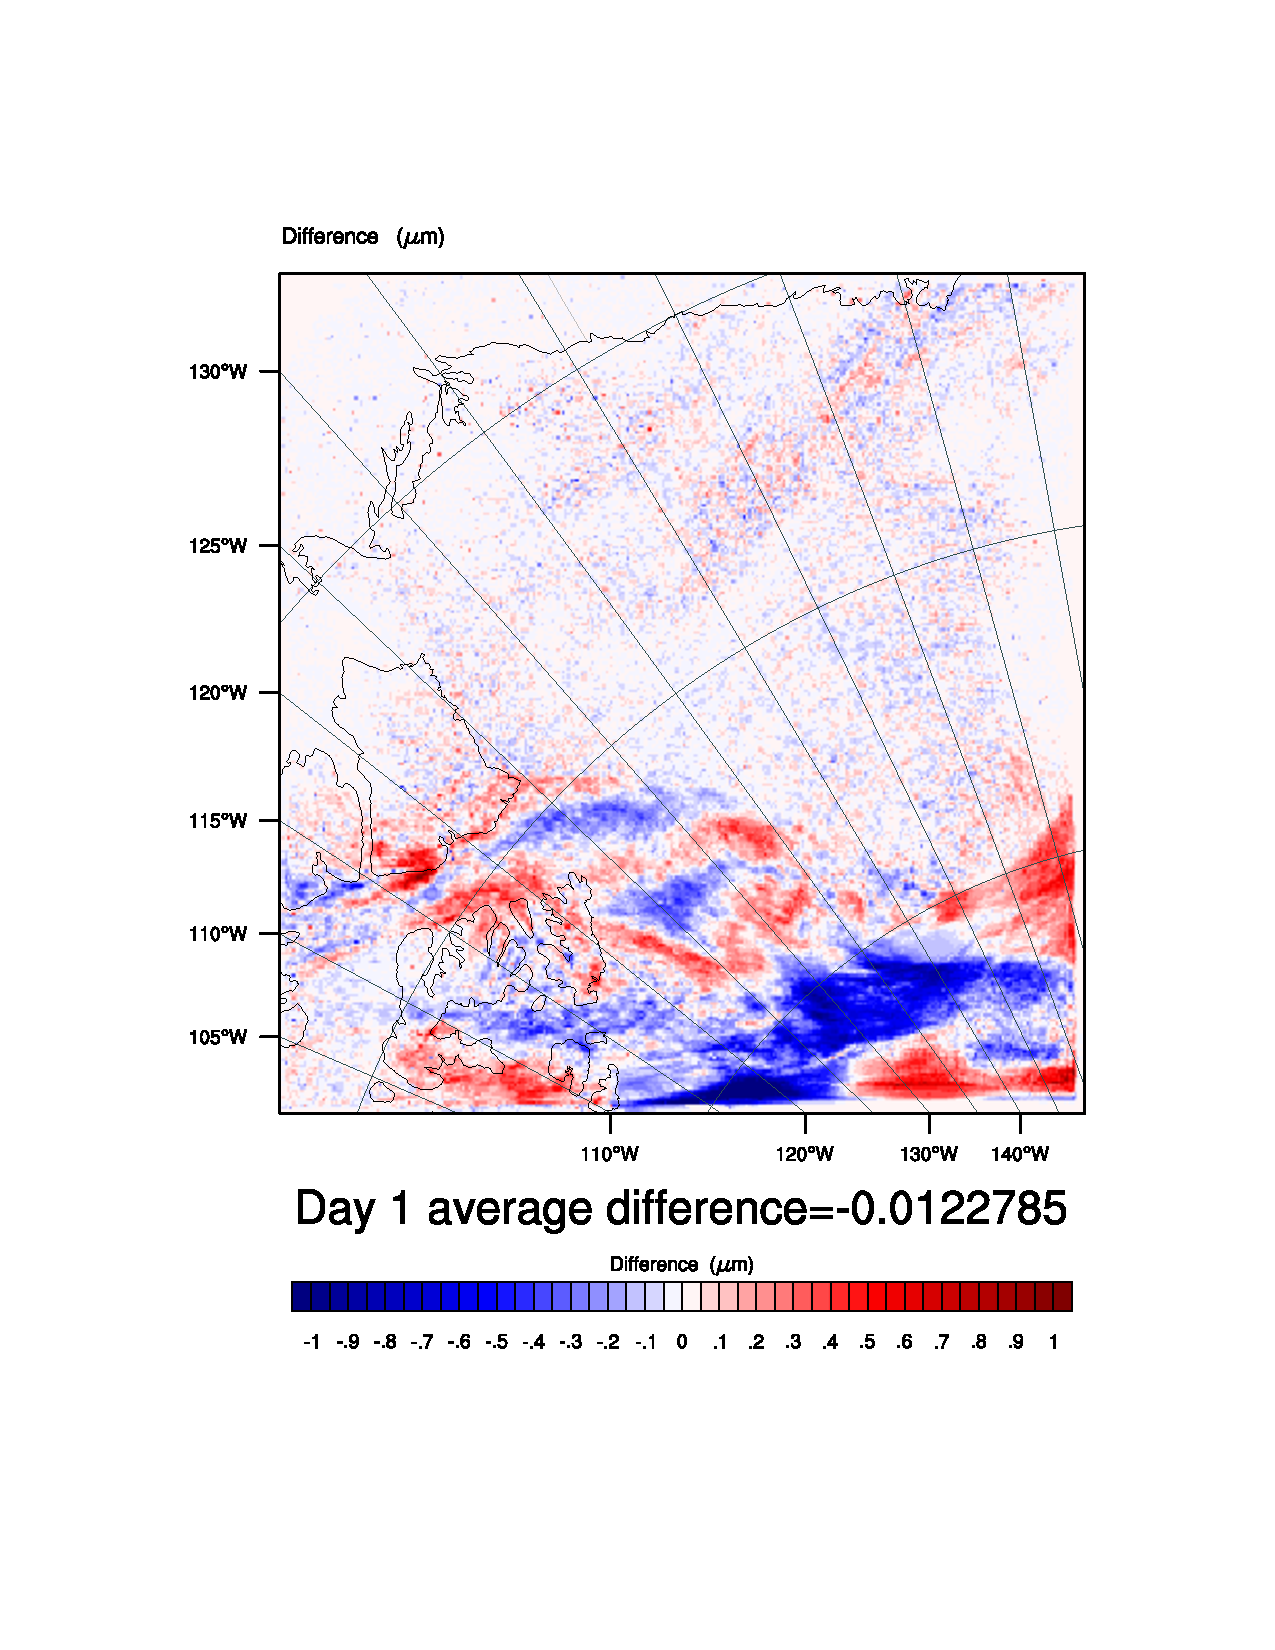
\includegraphics[width=\textwidth]{results/noice/diff_NoIce_RE_CLOUD_Day1.pdf}
		\caption{$r_e$, NoIce, day 1}
		\label{subfig:recloud_r2Day1}
	\end{subfigure}
\caption{The averaged difference in LWP, CDNC and $r_e$ of cloud droplets (from left to right) over the lowermost 11 layers for day 1. NoIce-Control.}
\label{fig:lwpcdncre_r2Day1}
\end{figure}

This implies that there is a new cloud forming in that area, that could not form when there was sea ice. The removal of the sea ice has allowed for increased evaporation and an increase in latent heat (LH) flux which can be seen from figure~\ref{subfig:lh_r2Day1}, where the shape of the area that sea ice was removed from is recognized.

\begin{figure}
\centering
	\begin{subfigure}{0.48\textwidth}
		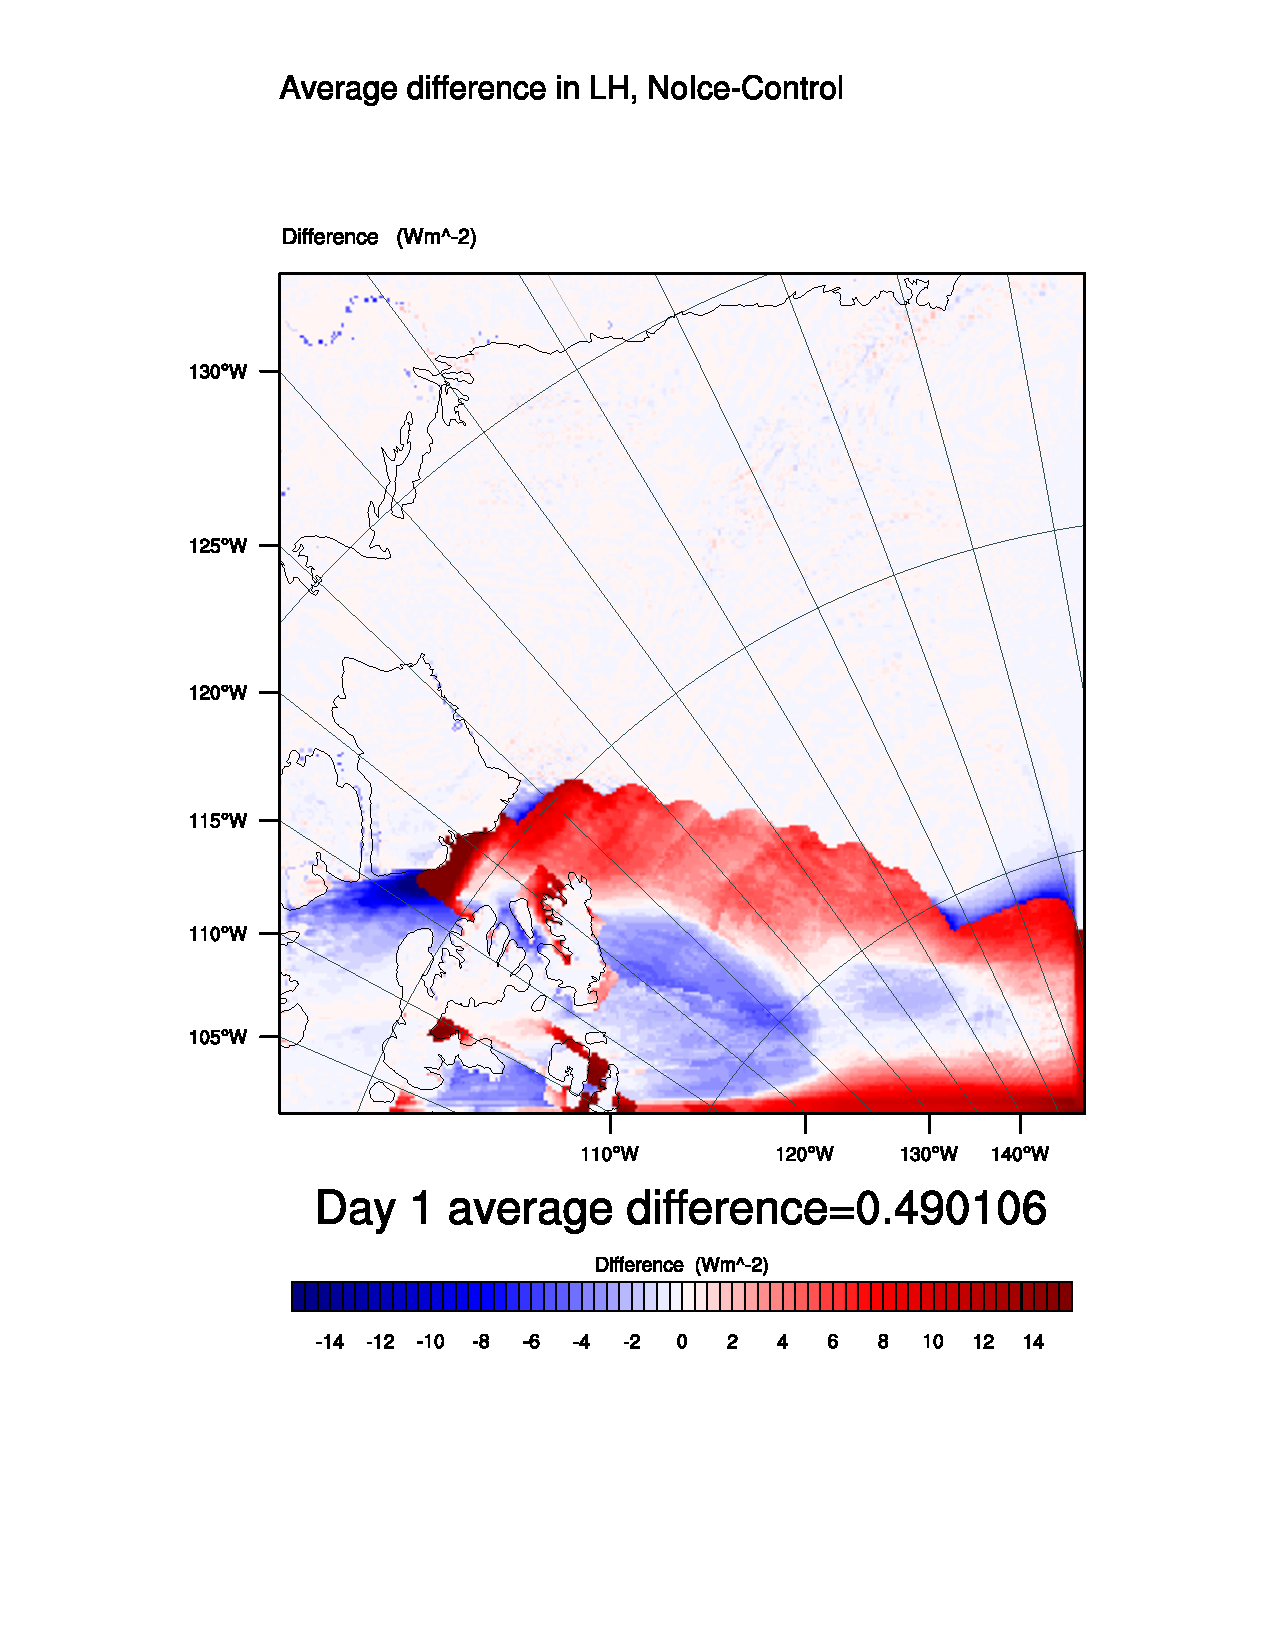
\includegraphics[width=\textwidth]{results/noice/diff_NoIce_LH_Day1.pdf}
		\caption{Difference in LH.}
		\label{subfig:lh_r2Day1}
	\end{subfigure}
	\quad
		\begin{subfigure}{0.48\textwidth}
		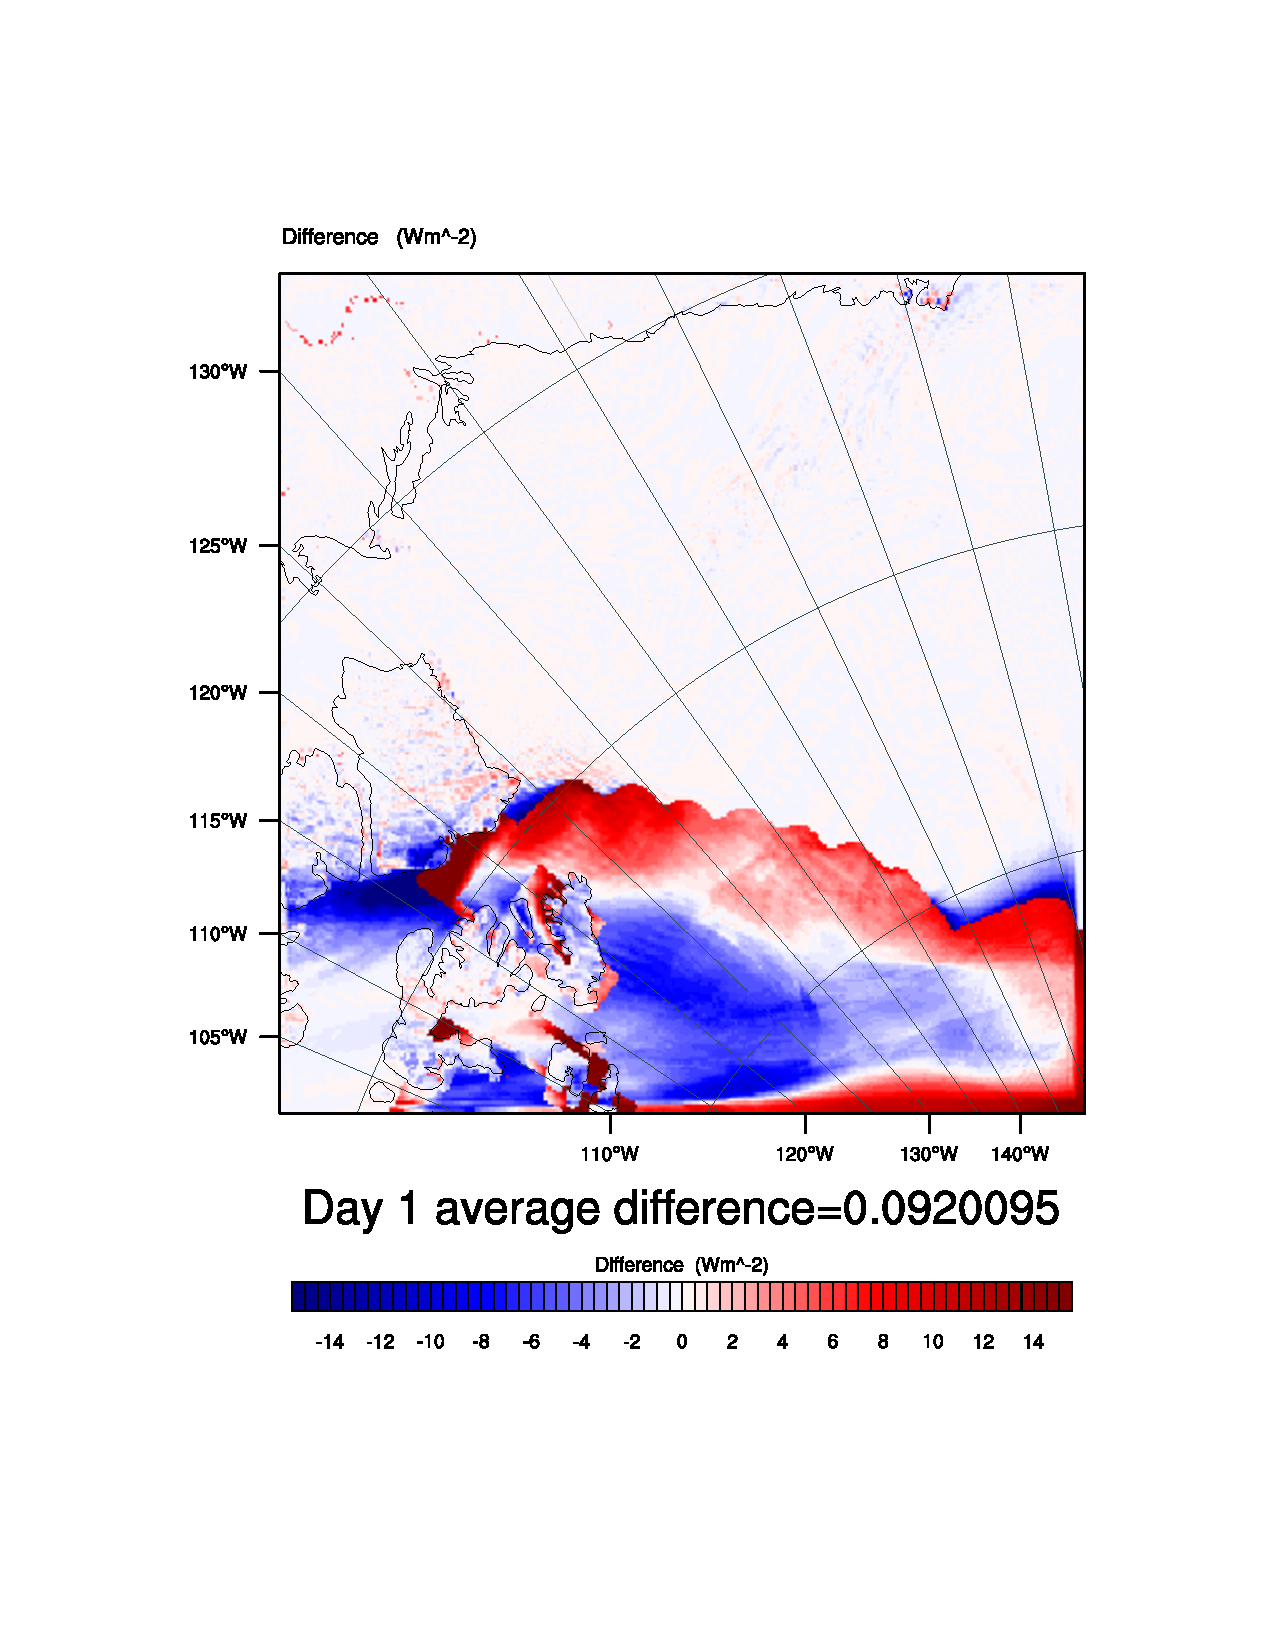
\includegraphics[width=\textwidth]{results/noice/diff_NoIce_HFX_Day1.pdf}
		\caption{Difference in SH.}
		\label{subfig:sh_r2Day1}
	\end{subfigure}
	
		\begin{subfigure}{0.48\textwidth}
		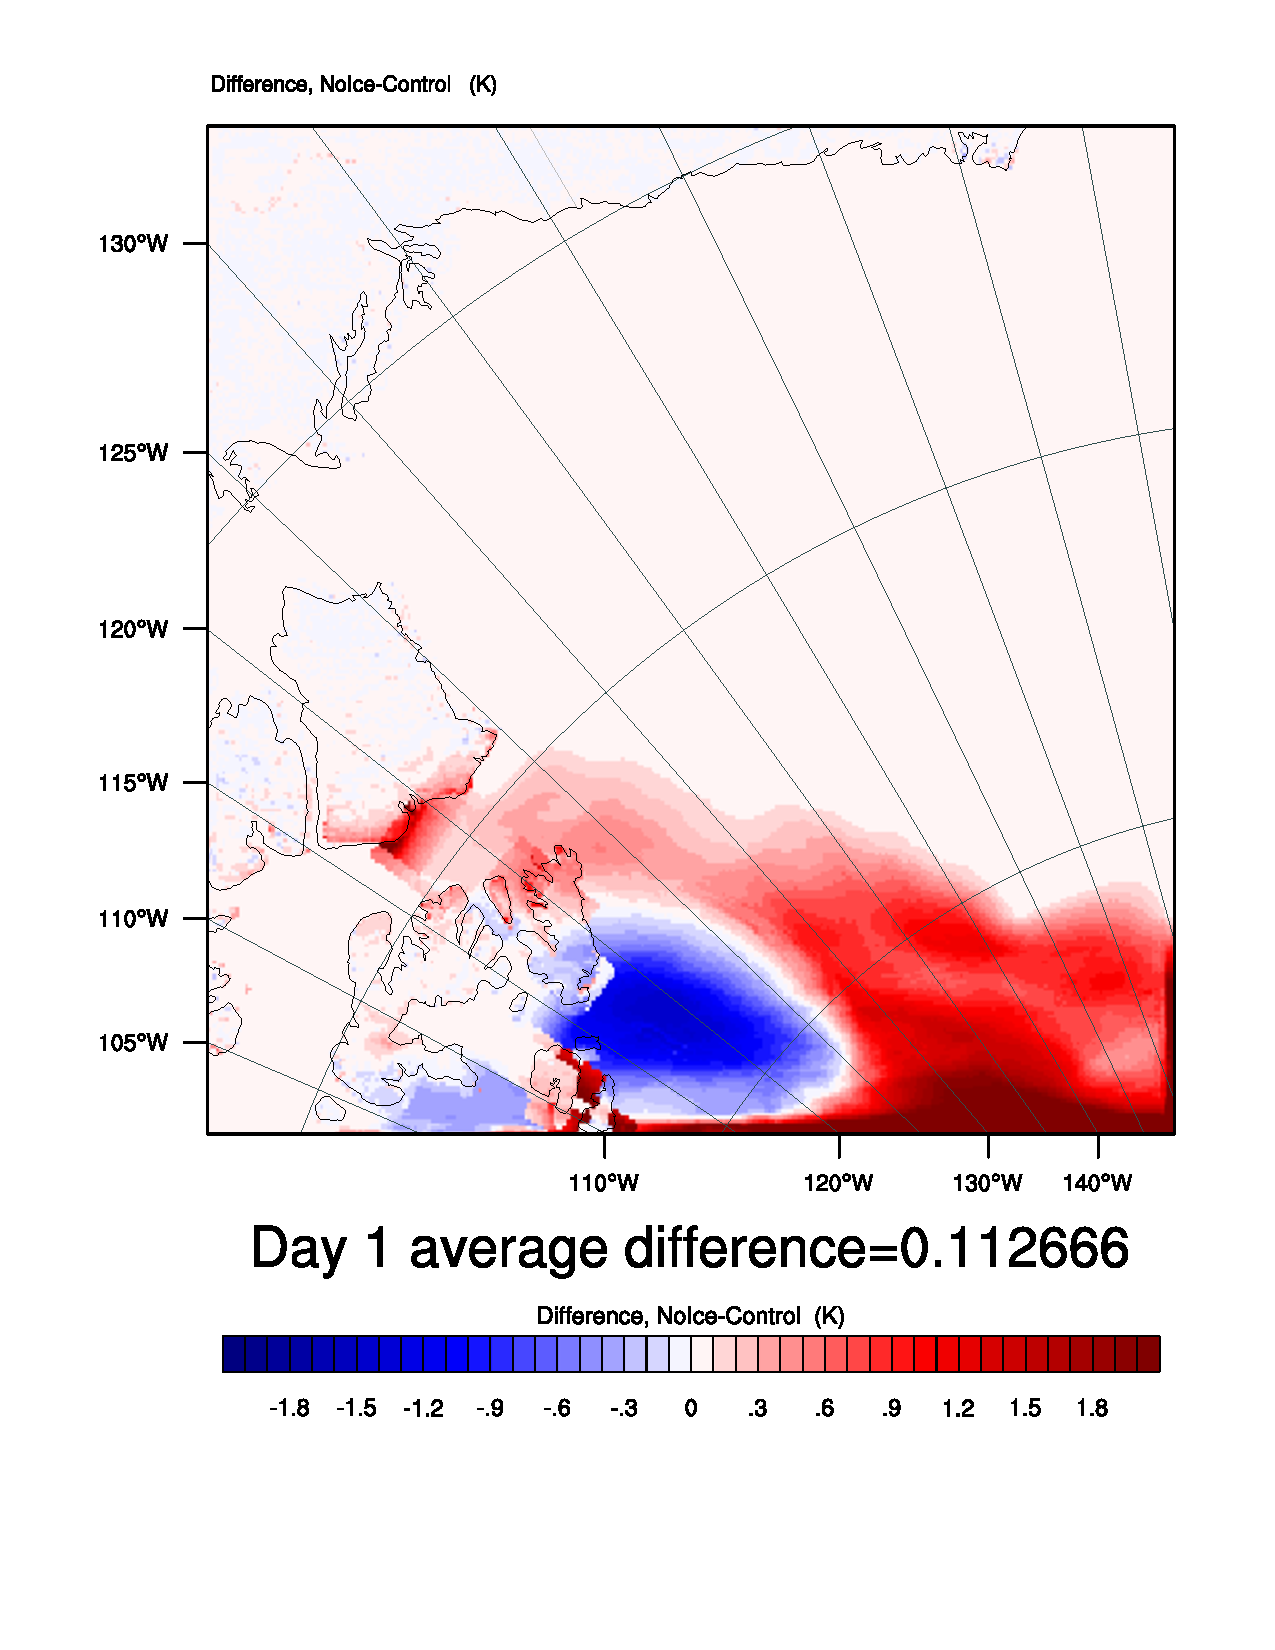
\includegraphics[width=\textwidth]{results/noice/diff_NoIce_skintemp_Day1.pdf}
		\caption{Difference in skin temperature.}
		\label{subfig:skin_r2Day1}
	\end{subfigure}
	\caption{Average difference in LH, SH and skin temperature for day1. NoIce-Control.}
	\label{fig:lhshskin_r2Day1}
\end{figure}

The northernmost part of the study area also has an increase in the cloud droplet number concentration (CDNC), figure~\ref{subfig:CDNCr2Day1}, in the same area as is covered by the red patch indicating an increase in the LWP, which fits well with equation~\ref{eqn:LWC}. There the amount of liquid water is proportional to the droplet number concentration, denoted by $N$ in the equation, and the LWP is the vertically integrated LWC. The average increase in the CDNC would be approximately 1 or 2 droplets per cubic centimeter in the northernmost area. The figure shows the numbers with units $10^6/\text{kg}$, which can be approximated to the more common units for CDNC, per cubic centimeter ($\text{cm}^{-3}$). Assuming that the cloud is close enough to the surface to assume a pressure $p=1000\text{hPa}$, and air density $\rho_a = 1\text{kg/m}^3=1\text{kg/}10^6\text{cm}^3$, then for CDNC $10^6/\text{kg} = \text{cm}^{-3}$ is a good approximation. Since CDNC is averaged over 24 hours and 11 layers (to a height of about 1600~m) the CDNC could be higher at certain times, and in certain layers.

The increase in effective radius in the same area as the LWP is increased also indicates the formation of a new cloud,figure~\ref{subfig:recloud_r2Day1}, that could not form in the control run (see figure~\ref{subfig:recloud_r1Day1}).

%The small "blob" at 140$^o$W and about 81$^o$N has decreased $r_e$, most likely because the cloud already was saturated in that area, which can be seen from the LWP from the control run, in figure~\ref{fig:LWPr1Day1}. The possible increase in aerosols from the ocean that would then lead to an increase in CCN would make the water in that cloud spread over more CCN, and by that leave the droplets with a smaller $r_e$.

The the two red patches at 80$\degree$N and 140-155$\degree$W in the figure for difference in $r_e$, figure~\ref{subfig:recloud_r2Day1}, are also clear in the difference in LW downward radiation, figure~\ref{subfig:glw_r2Day1} at the ground surface, and can also be slightly recognized as a decrease in SW downward radiation, figure~\ref{subfig:swdown_r2Day1}. The SW radiation flux at ground surface has been reduced due to the increase in LWP, and the more pronounced decrease in SW is clearly recognized with the same shape and size as the northern patch of increase in LWP. This can be explained by equations~\ref{eqn:cloudalbedo} and~\ref{eqn:cloudtau}, where it is clear from equation~\ref{eqn:cloudtau} that the cloud optical depth, $\tau$, increases with LWP, and following equation~\ref{eqn:cloudalbedo} an increase in $\tau$ would also increase the cloud albedo.

\begin{figure}
\centering
	\begin{subfigure}{0.48\textwidth}
		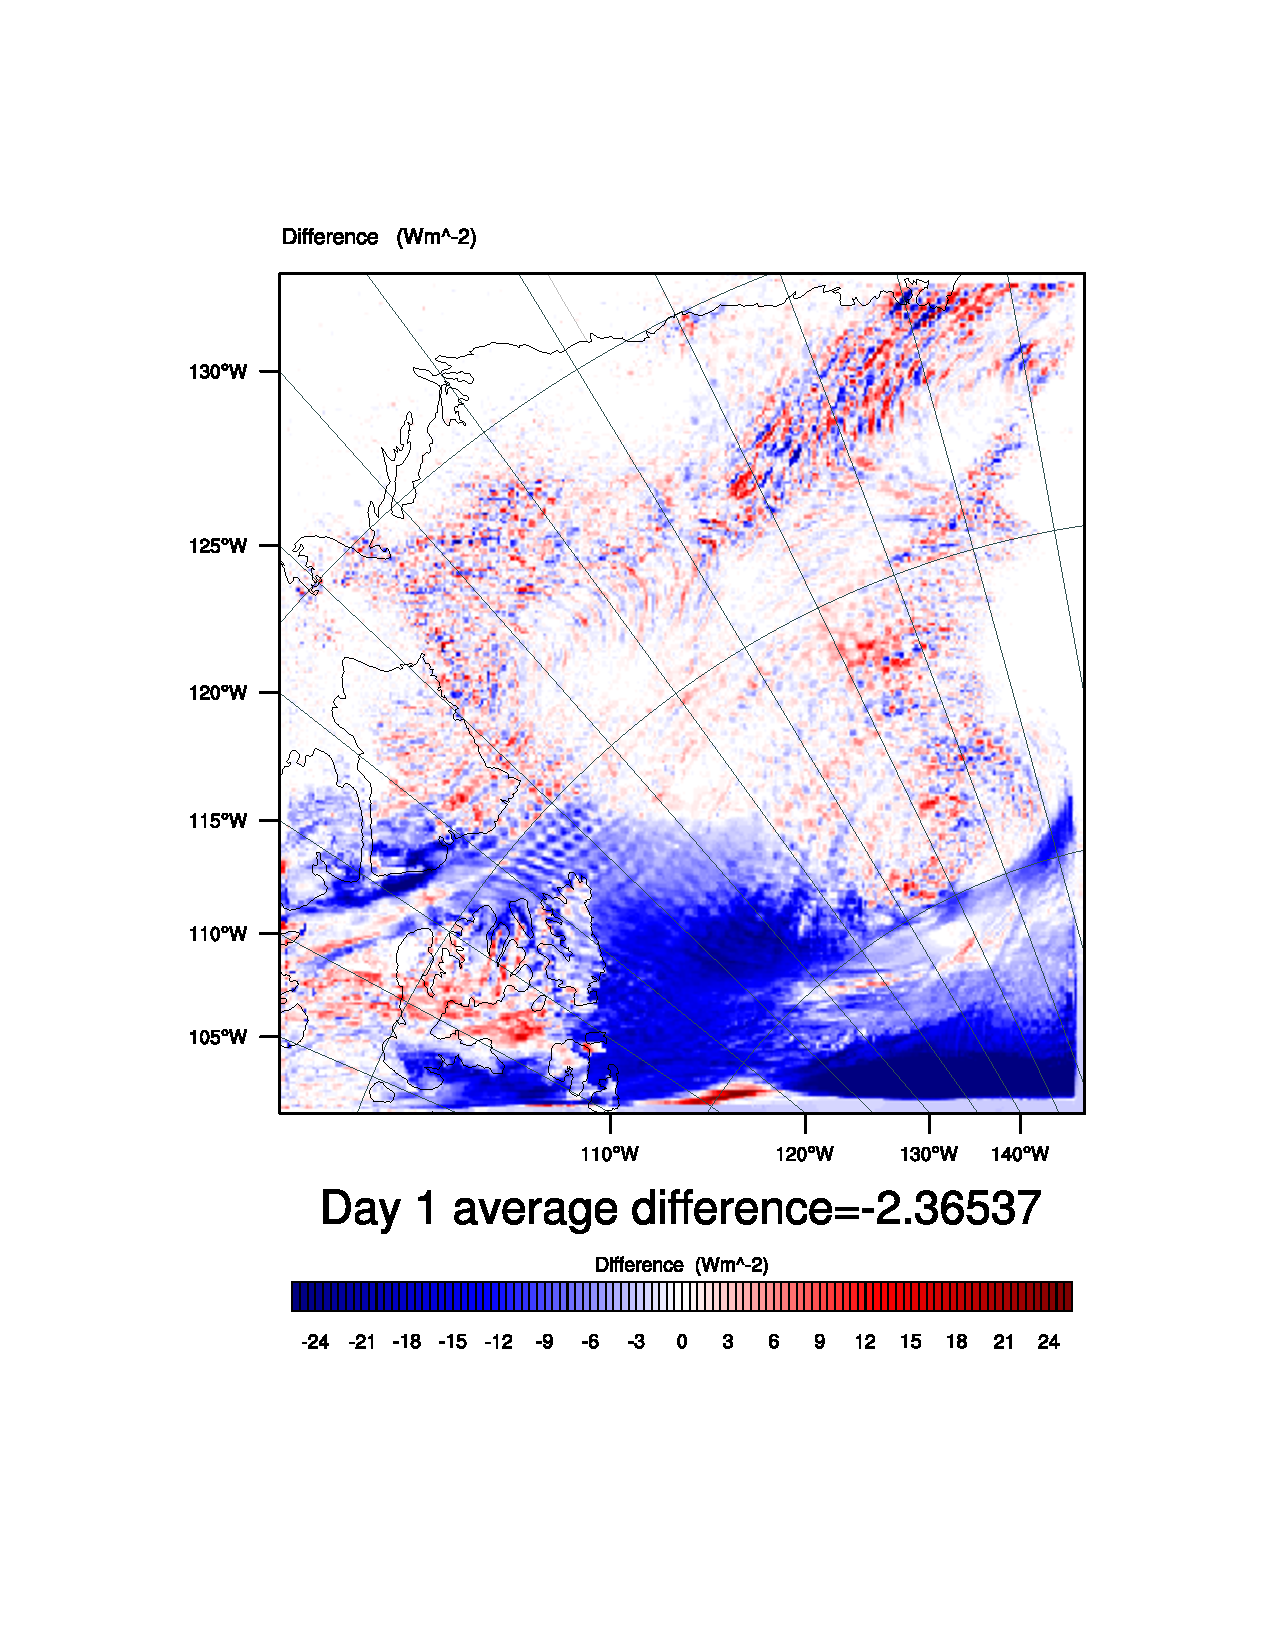
\includegraphics[width=\textwidth]{results/noice/diff_NoIce_SWDOWN_Day1.pdf}
		\caption{The average difference in SW flux down at the surface, day 1.}
		\label{subfig:swdown_r2Day1}
	\end{subfigure}
	\quad
	\begin{subfigure}{0.48\textwidth}
		\centering
		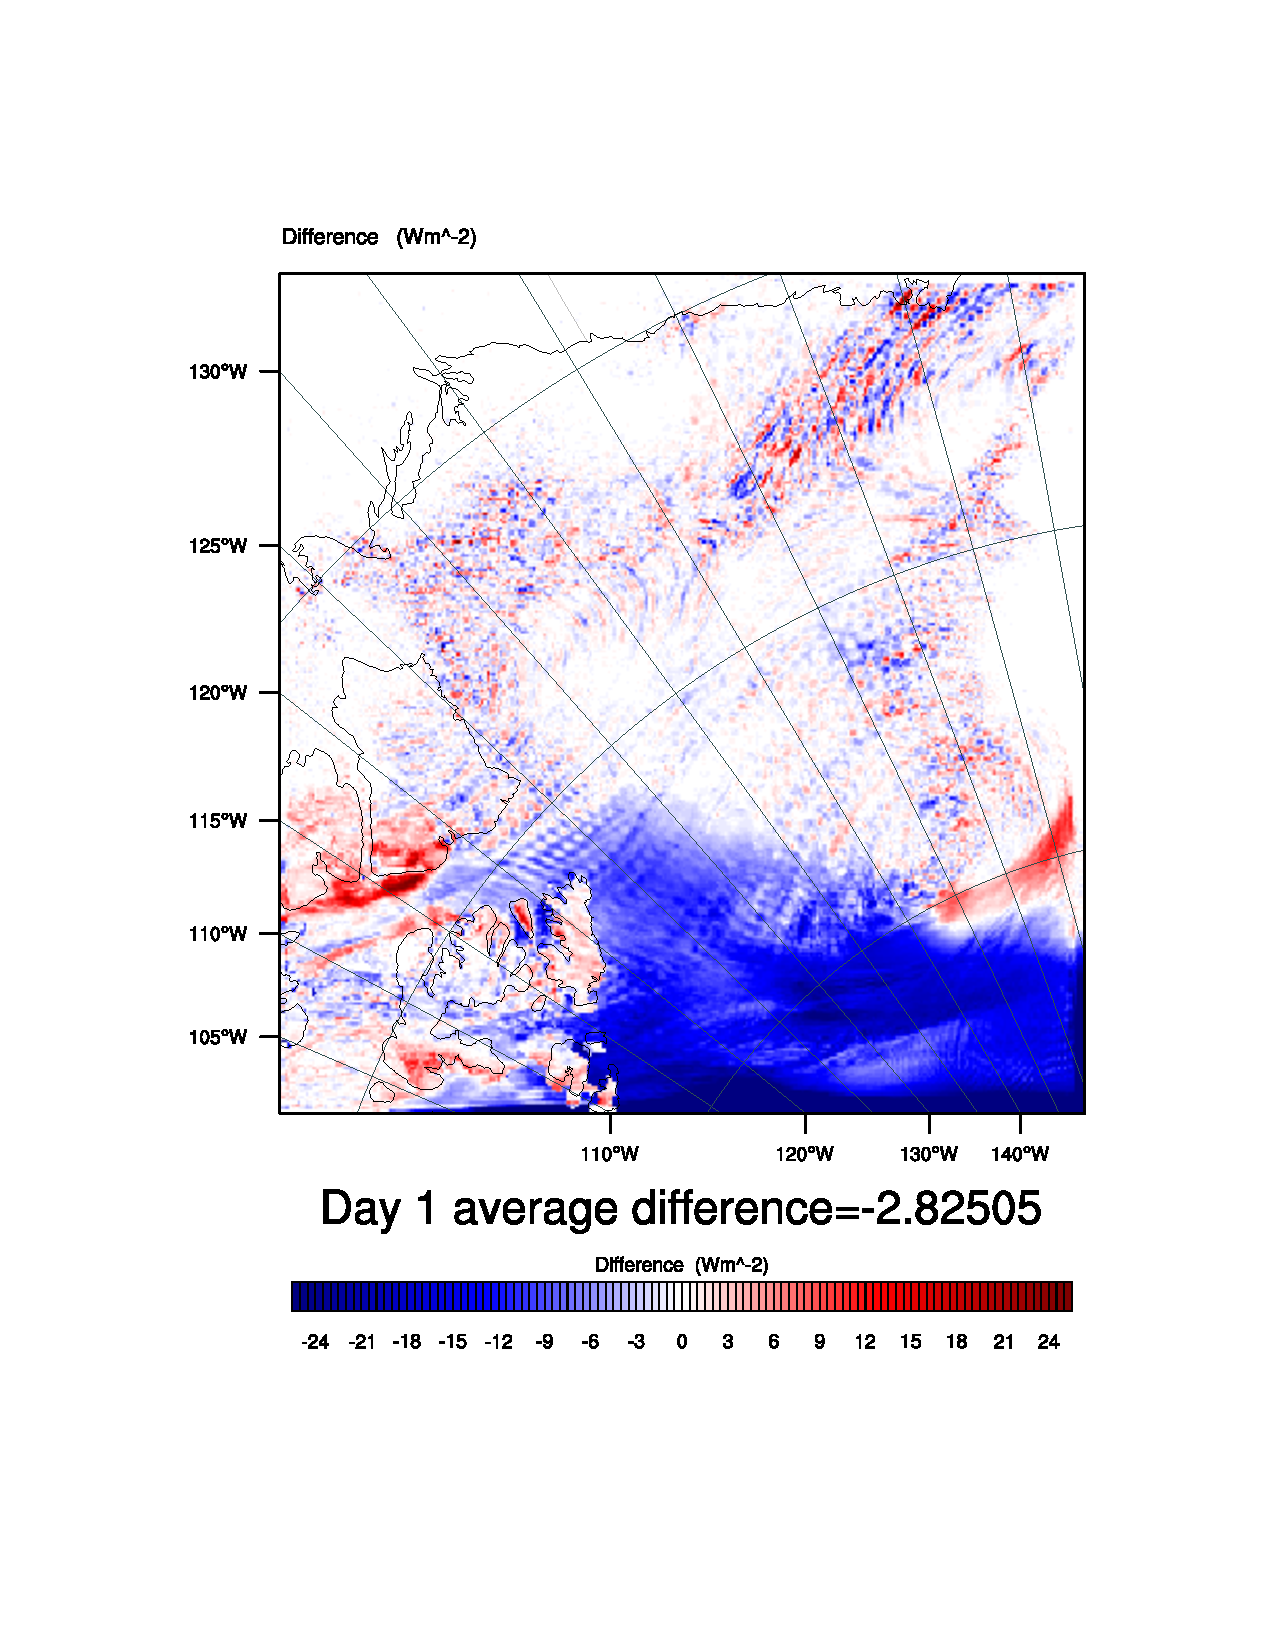
\includegraphics[width=\textwidth]{results/noice/diff_NoIce_SWUPT_Day1.pdf}
		\caption{The average difference in SW flux up at TOA, day 1.}
		\label{subfig:swup_r2Day1}
	\end{subfigure}
	
	\begin{subfigure}{0.48\textwidth}
		\centering
		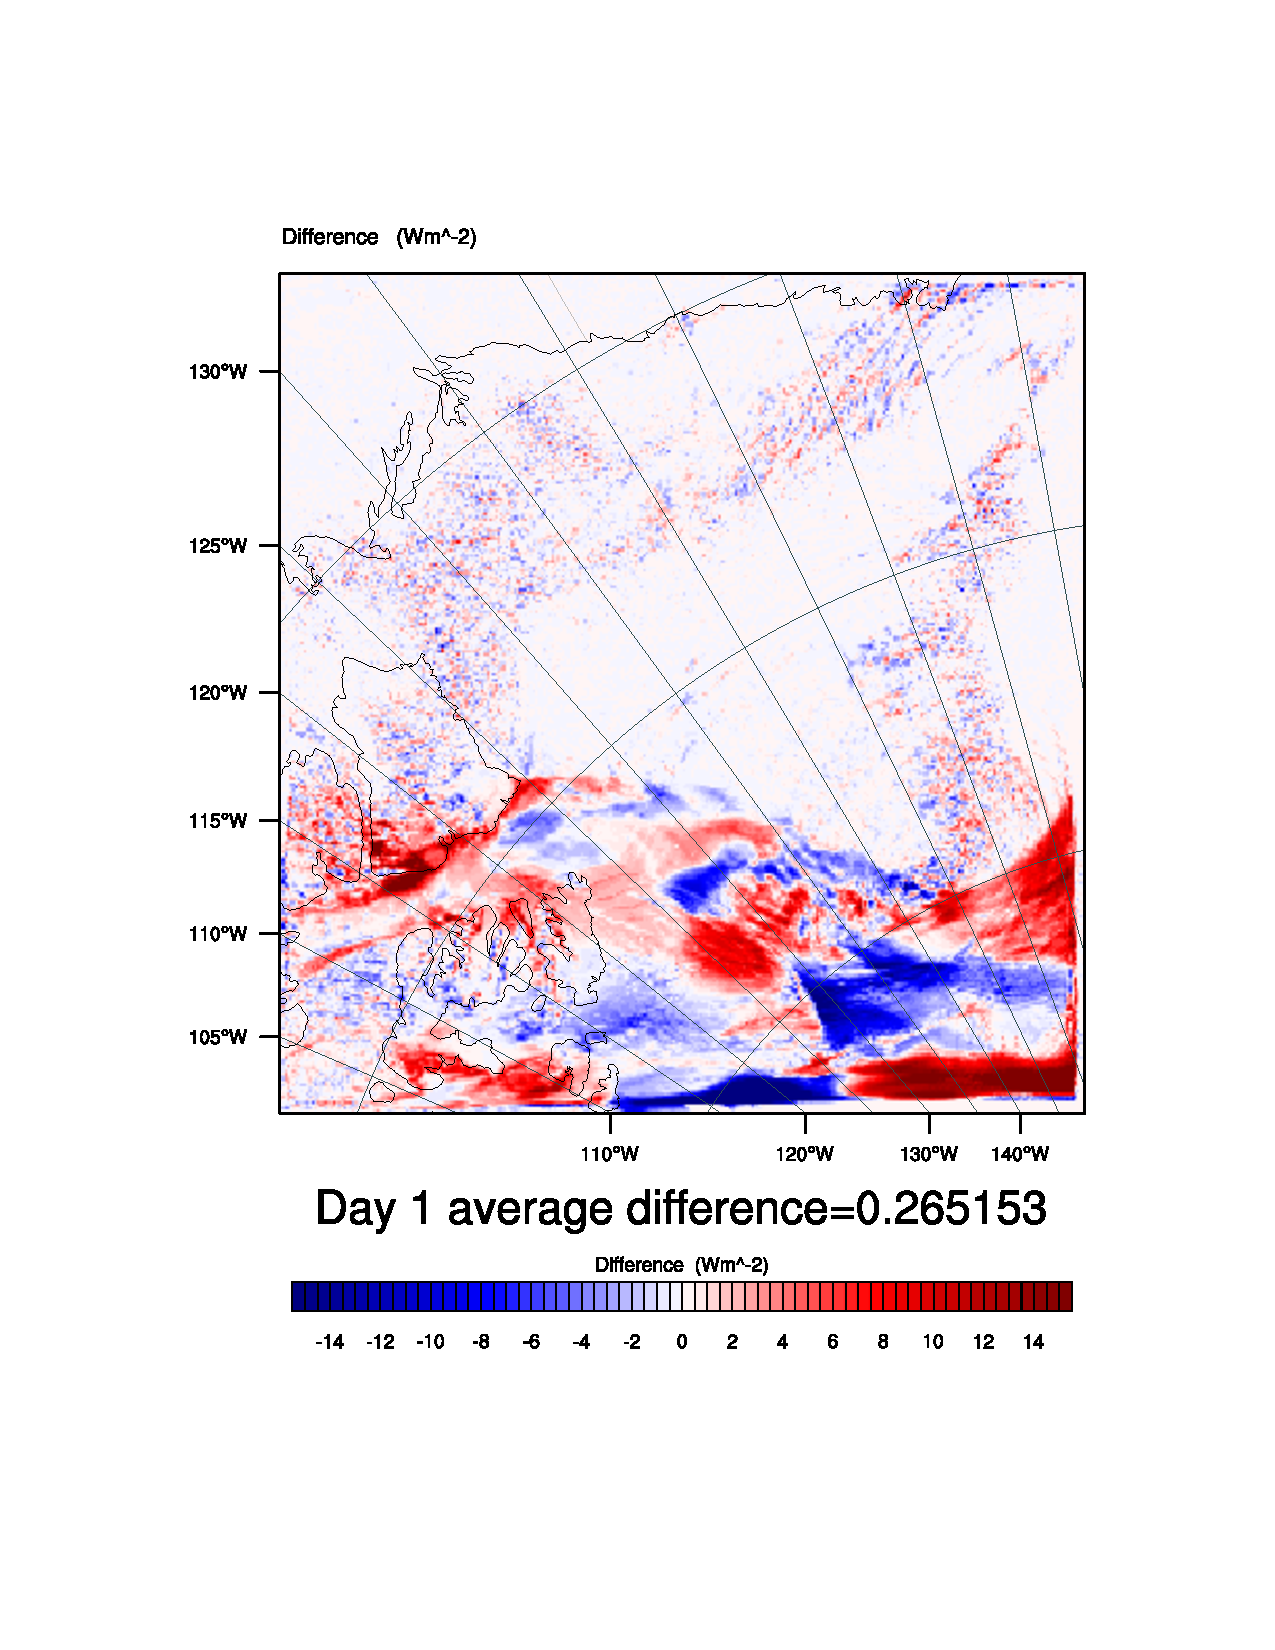
\includegraphics[width=\textwidth]{results/noice/diff_NoIce_GLW_Day1.pdf}
		\caption{The average difference in LW flux down at the surface, day 1.}
		\label{subfig:glw_r2Day1}
	\end{subfigure}
	\quad
	\begin{subfigure}{0.48\textwidth}
		\centering
		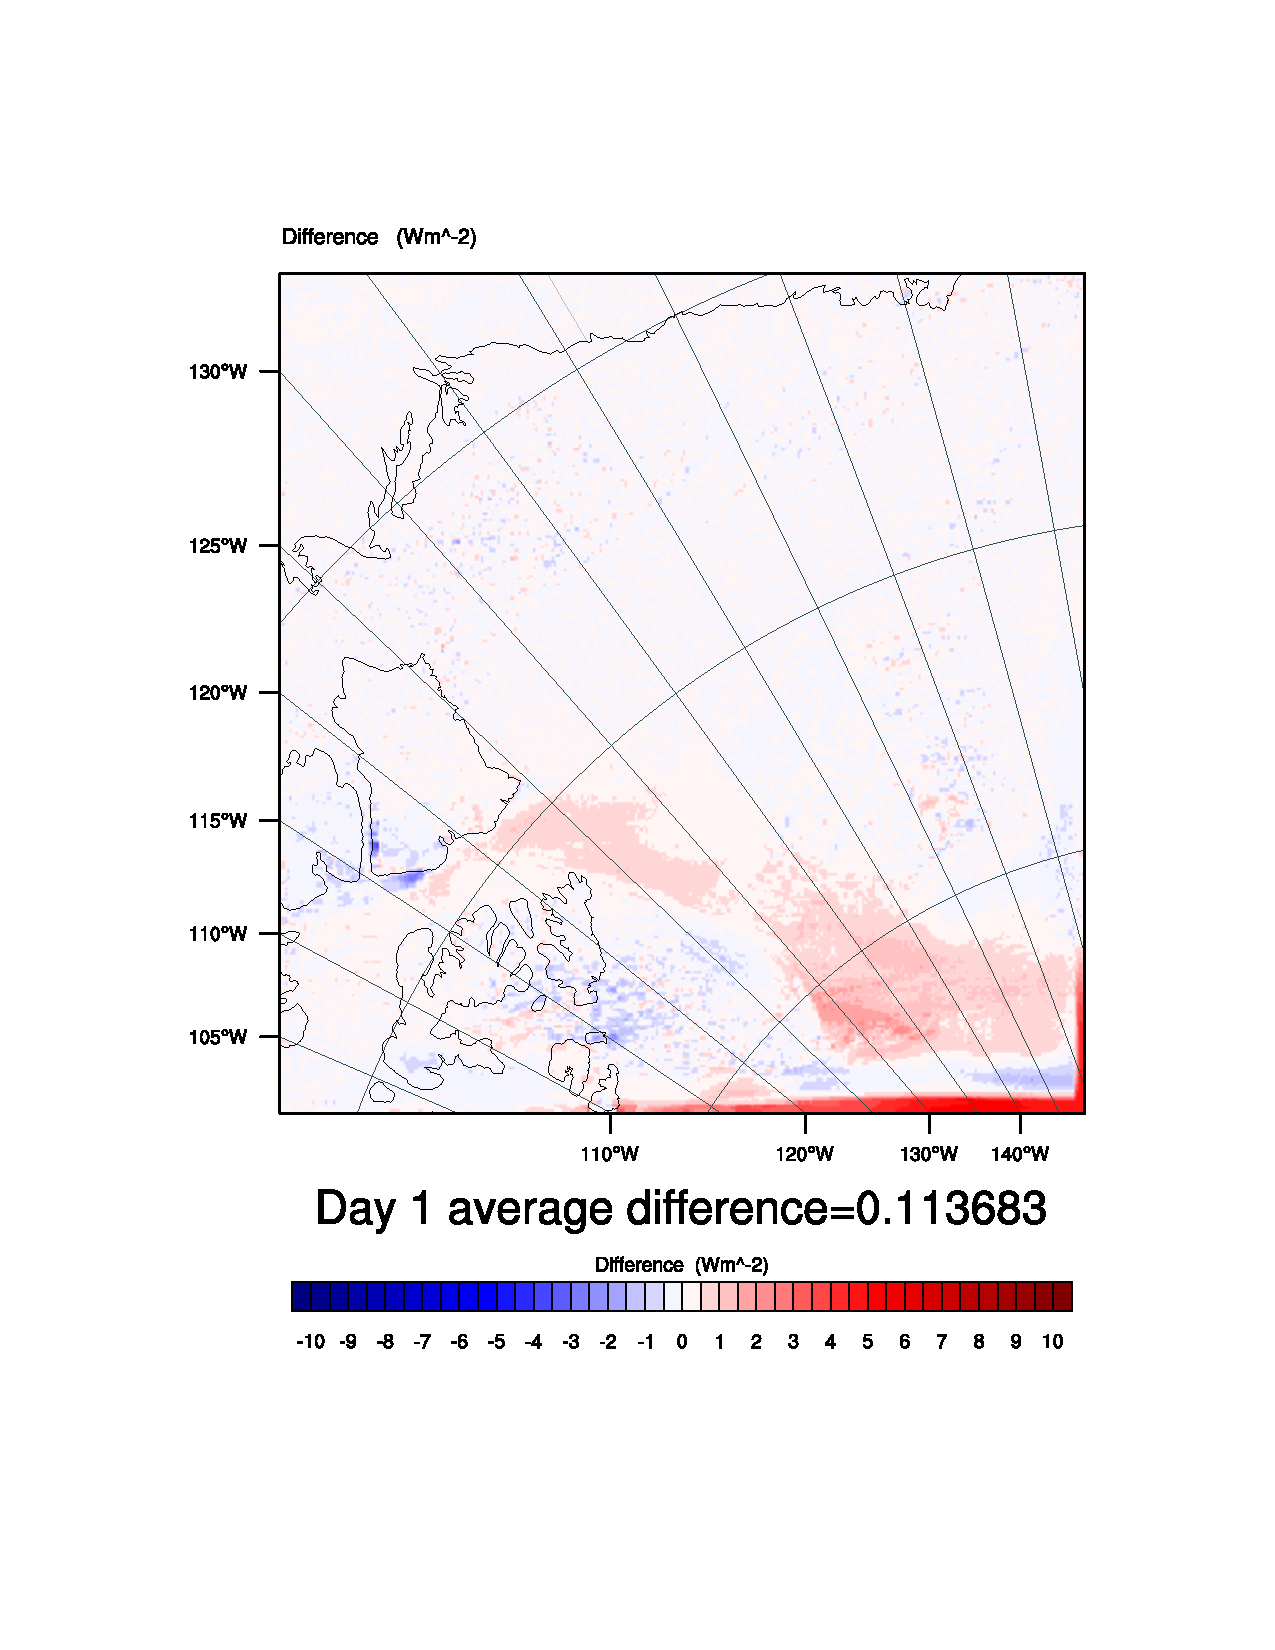
\includegraphics[width=\textwidth]{results/noice/diff_NoIce_LWUPT_Day1.pdf}
		\caption{The average difference in LW flux up at TOA, day 1.}
		\label{subfig:lwup_r2Day1}
	\end{subfigure}
	\caption{The average difference in SW and LW flux down at the surface and up at TOA, for day 1. NoIce-Control.}
	\label{fig:radiation_r2Day1}
\end{figure}

The downward LW radiation flux at the surface (figure~\ref{subfig:glw_r2Day1}) has been increased due to the increase in LWP, which means that there is more water in the clouds and they emit more LW to the ground. It was shown in Chapter~\ref{chap:theory} that an increase in LWP increases the emissivity of the cloud, shown in equation~\ref{eqn:epsilon_lw}, until the cloud is saturated with respect to LW radiation at about 40-45$\text{g/m}^2$, following figure~\ref{fig:epsalb}.
The slight increase in the LW at TOA is because of increased temperature at the surface when the sea ice is removed (figure~\ref{subfig:skin_r2Day1}).

%The LW at the top of the atmosphere (TOA) does not experience such an increase, in fact it experiences a slight decrease. That it doesn't experience the same increase is explained by the Stefan-Boltzmann's law presented in chapter~\ref{chap:theory}, where the flux density emitted by a body, in this case a cloud, is dependent on the temperature and emissivity of the body (equation~\ref{eqn:stefanboltzmann}).
%The temperature contours in figure~\ref{subfig:cross_LWC_day1}, from the control run, show that the temperature decreases with height and that the clouds hold a lower temperature than there is close to the sea ice. In the run with no ice, the situation is the same (see figure~\ref{subfig:cross_LWC_r2day1}), therefore if clouds with lower temperatures than the surface are the source of the LW reaching TOA the LW reaching TOA would be lower.
%The removal of sea ice has a larger effect on lower clouds than on higher clouds, since the increase in evaporation from the surface doesn't reach high up in the troposphere, especially not in the Arctic, due to the static stability of the lower atmosphere in the Arctic(@cite someone?). Also the LWP showed in this study is only for the lowermost 11 layers and can only explain what happens in those layers, it can not be used as a final explanation for radiation changes that are only at the bottom and top of the modeled atmosphere.
%--------------

Of course, the removal of sea ice would reduce the SW at TOA, see figure~\ref{subfig:swup_r2Day1}. The albedo of sea ice varies between 0.5 and 0.9 depending on snow cover and the age of the ice and is typically 0.5-0.7 for bare ice, whereas a typical ocean albedo is 0.06~\citep{NSIDC}. Thus the change in SW at TOA is negative over the area of ocean where there was sea ice in the control run. The increased SW at TOA at 80$\degree$N and 155$\degree$W is because of the cloud forming in that area, see figure~\ref{subfig:swup_r2Day1}, and can be recognized in the increase in $r_e$ in the same place (figure~\ref{subfig:recloud_r2Day1}) which also represent an increase in LWP and reduction in SW at surface and increase of LW at surface. This is due to the enhanced albedo caused by new clouds at that location, since these figures don't show in-cloud changes, simply the difference between the fields from the run without ice and the control run.

The heat fluxes are almost unchanged for most of the study area by the removal of sea ice, except for the area where the sea ice has been removed (see figures~\ref{subfig:lh_r2Day1} and~\ref{subfig:sh_r2Day1}). Especially for the northernmost part of the study area and "sea ice removed area" the fluxes are a lot higher than in the control run. This is not surprising, since one would expect the ocean surface to hold a higher temperature than the sea ice, therefore more heat is released than in the case when sea ice is present. 

%----------------
\clearpage
\subsection{Day 5}
%----------------
The average differences for LWP, CDNC and $r_e$ at day 5 are all negative, see figure~\ref{fig:lwpcdncre_r2Day5}, over the area that had ice in the control run. Thus the clouds making up the LWP in the control run, see figure~\ref{subfig:LWPr1Day5}, have either ceased to exist, been significantly thinned, moved away or turned into ice. The LWP has a negative difference of >30~$\text{g/m}^2$, which means that the LWP, when comparing with the values for that area in the control run (figure~\ref{subfig:LWPr1Day5}) which were around 40-100~$\text{g/m}^2$, there is still around 20-70$\text{g/m}^2$ left. So the clouds have not all ceased to exist. This is supported by the fact that the CDNC in the control run was $\sim$10 to 25~$\text{cm}^{-3}$ and has according to figure~\ref{subfig:CDNCr2Day5} got 3 to >5 droplets~$\text{cm}^{-3}$ less in the run with no ice. Then the clouds in the run with no ice are left with <5 to around 20 droplets~$\text{cm}^{-3}$ which is definitely enough to assume that there are still clouds in the area.

\begin{figure}[hb]
\centering
	\begin{subfigure}{0.32\textwidth}
		\centering
		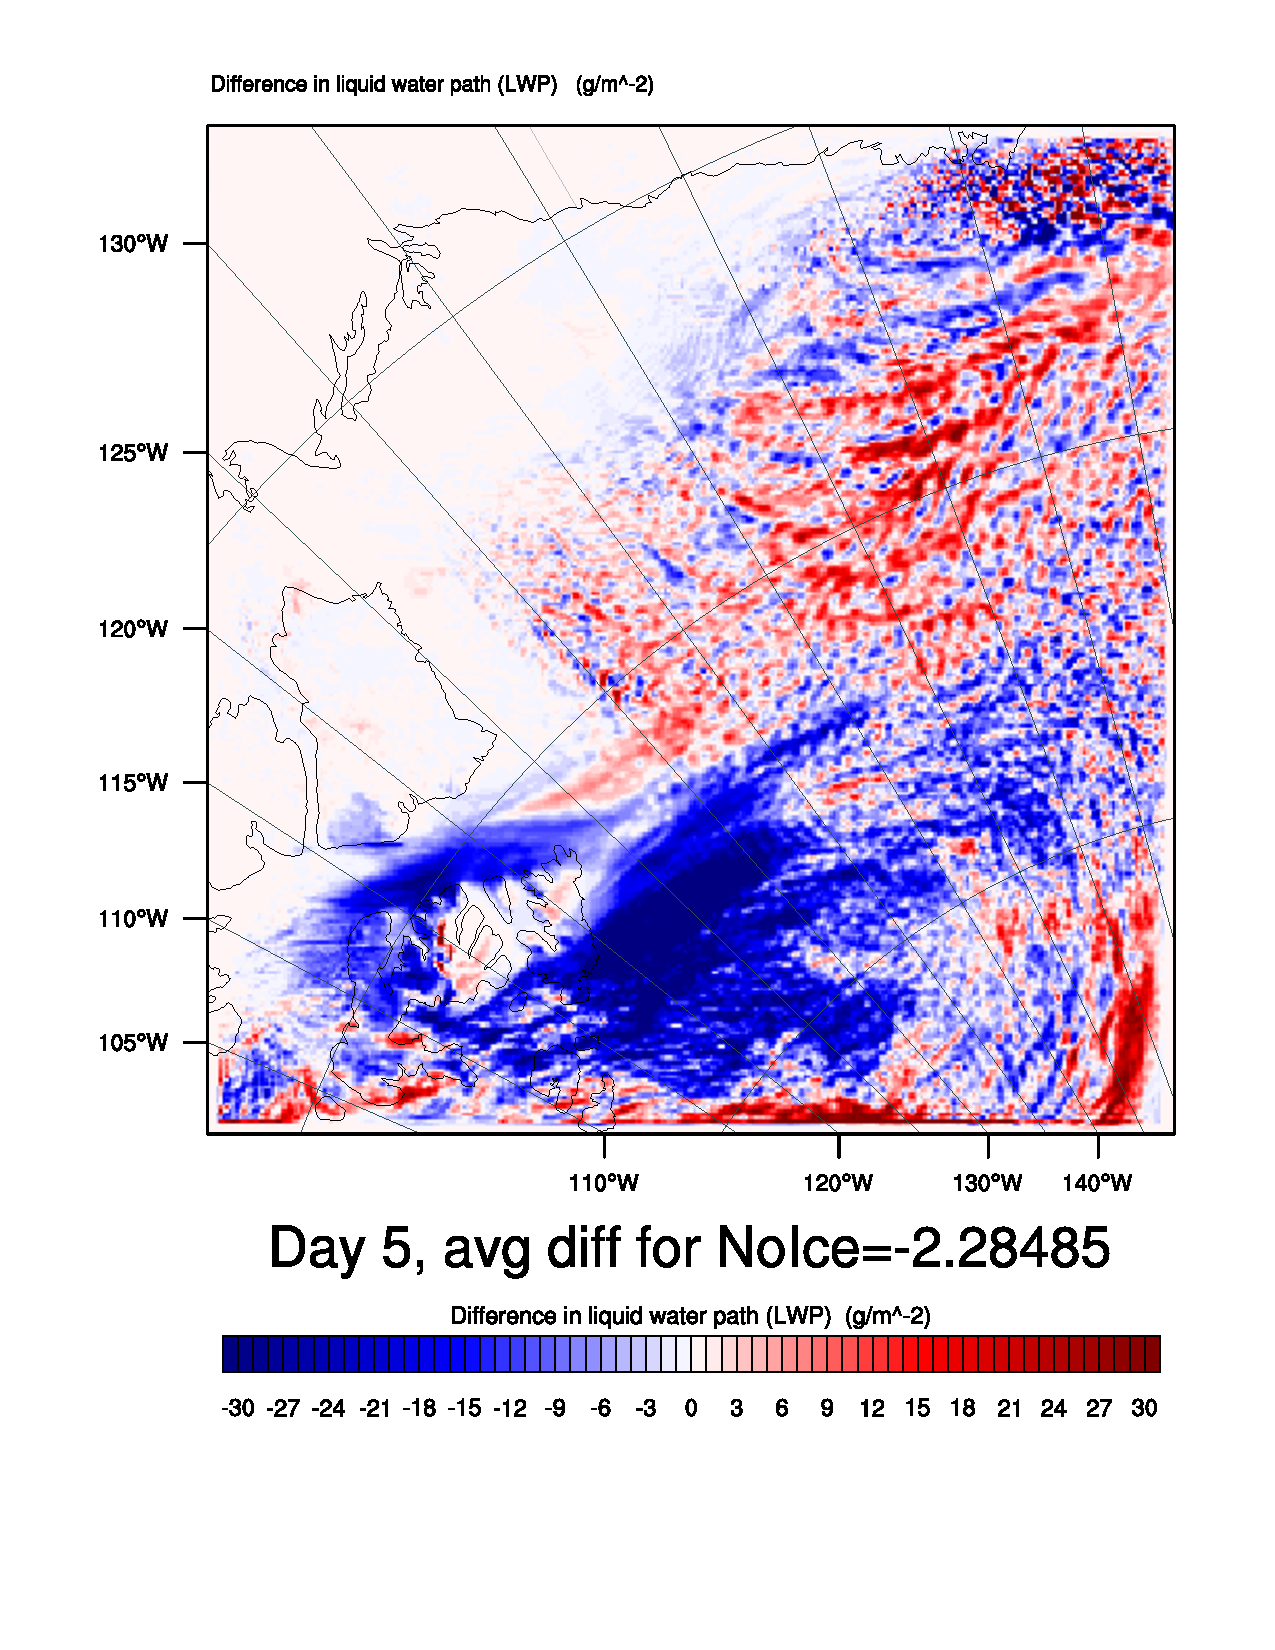
\includegraphics[width=\textwidth]{results/noice/Diff_LWP_Day5NoIce.pdf}
		\caption{LWP, NoIce, day 5}
		\label{subfig:LWPr2Day5}
	\end{subfigure}
	\begin{subfigure}{0.32\textwidth}
		\centering
		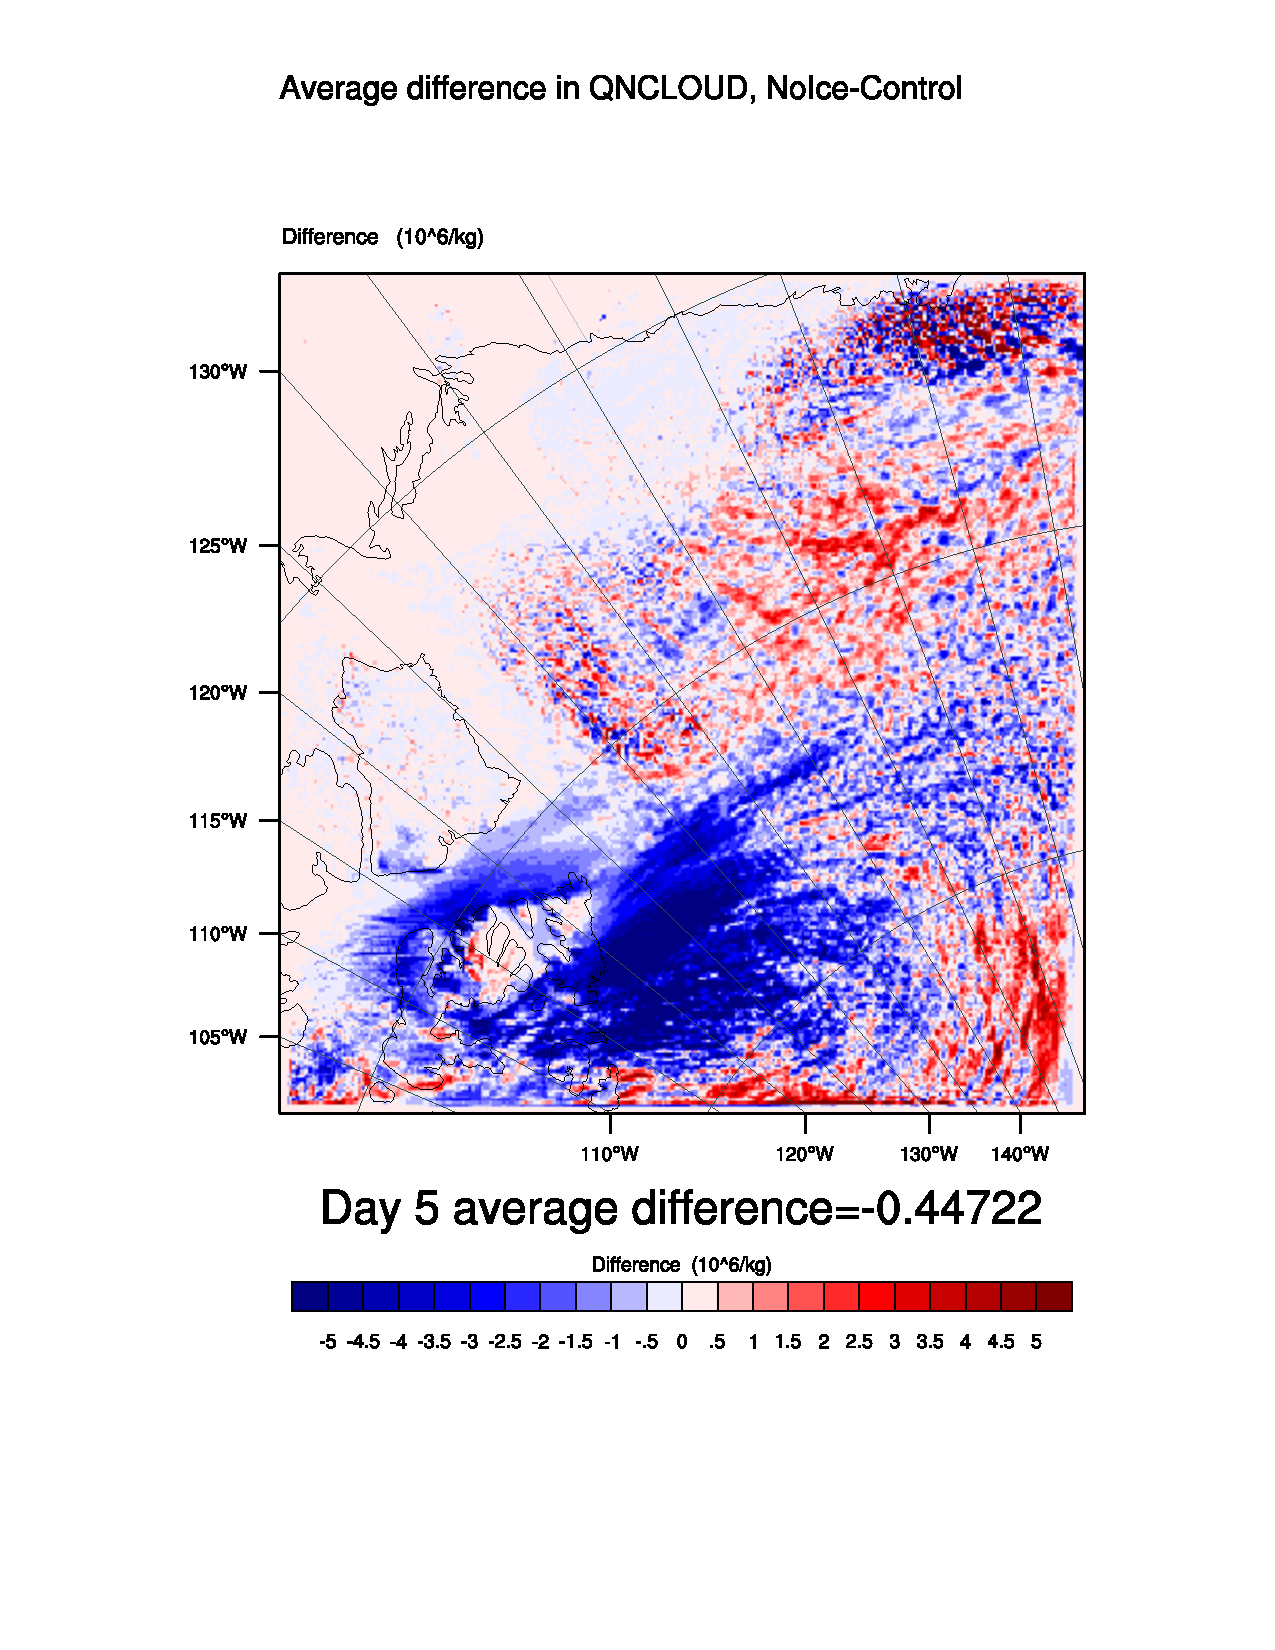
\includegraphics[width=\textwidth]{results/noice/diff_NoIce_QNCLOUD_Day5.pdf}
		\caption{CDNC, NoIce, day 5}
		\label{subfig:CDNCr2Day5}
	\end{subfigure}
	\begin{subfigure}{0.32\textwidth}
		\centering
		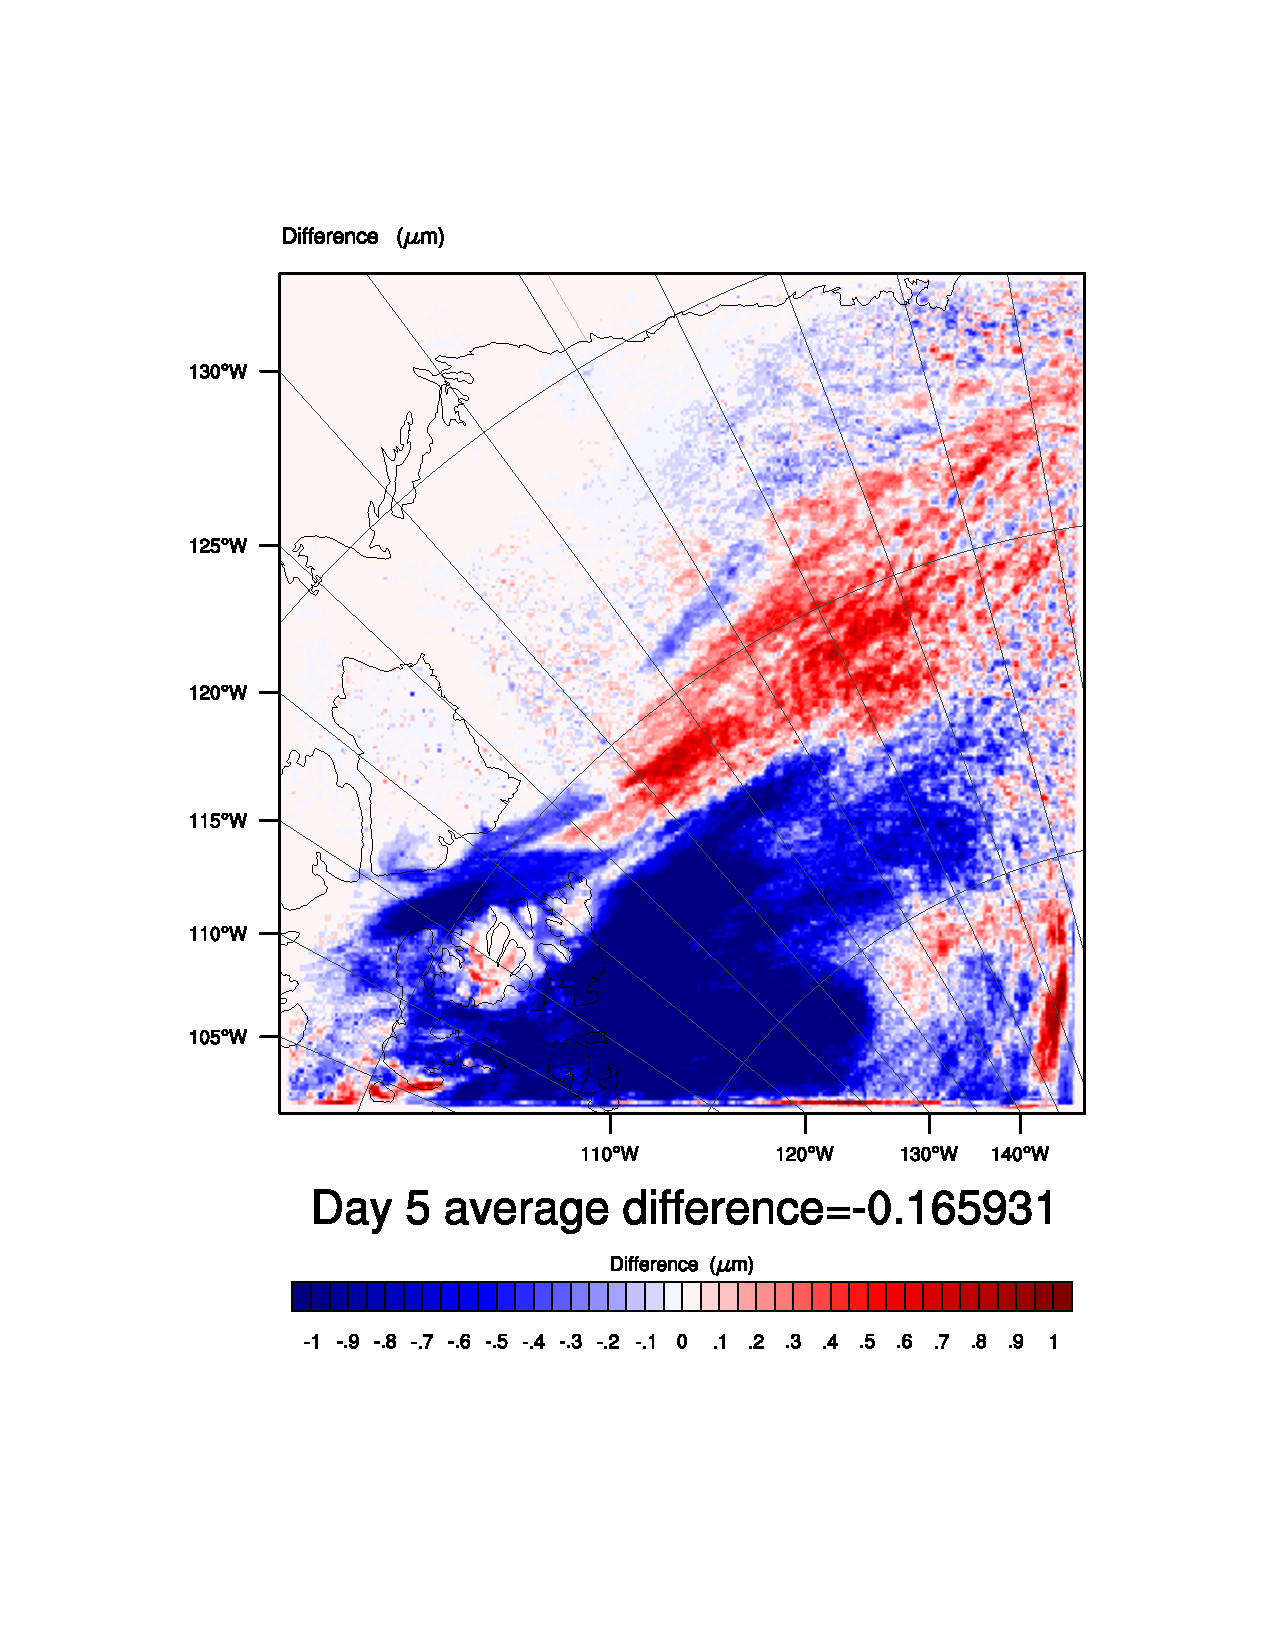
\includegraphics[width=\textwidth]{results/noice/diff_NoIce_RE_CLOUD_Day5.pdf}
		\caption{$r_e$, NoIce, day 5}
		\label{subfig:recloud_r2Day5}
	\end{subfigure}
\caption{The average difference in LWP, CDNC and $r_e$ of cloud droplets (from left to right) over the lowermost 11 layers for day 1. NoIce-Control.}
\label{fig:lwpcdncre_r2Day5}
\end{figure}

There is hardly any ice at all in the study area in the lowermost 11 layers, much like in the control run (see figure~\ref{subfig:cinc_cont_Day5}), and the IWP is zero (not shown) over the area where there was sea ice, and the area around. The wind pattern (not shown) is very much the same as in the control run (figure~\ref{subfig:weather_cont_day5}), and the chance that the clouds have been moved to a different area is ruled out. Therefore precipitation must have depleted the clouds of some of droplets. The difference in rain (not shown) for the run with no ice compared to the control run is negligible and so snow was found guilty of depleting the clouds. Figure~\ref{fig:snowstory} shows how the cloud that was claimed started to form in day 1 of the run with no ice, in section~\ref{sec:noiceDay1}, as more water vapor and aerosols were made available, develops into a snowing cloud and performs natural cloud seeding by snowing out the other clouds as it travels south-east over the sea ice free area.

\begin{figure}
\centering
	\begin{subfigure}{0.32\textwidth}
		\centering
		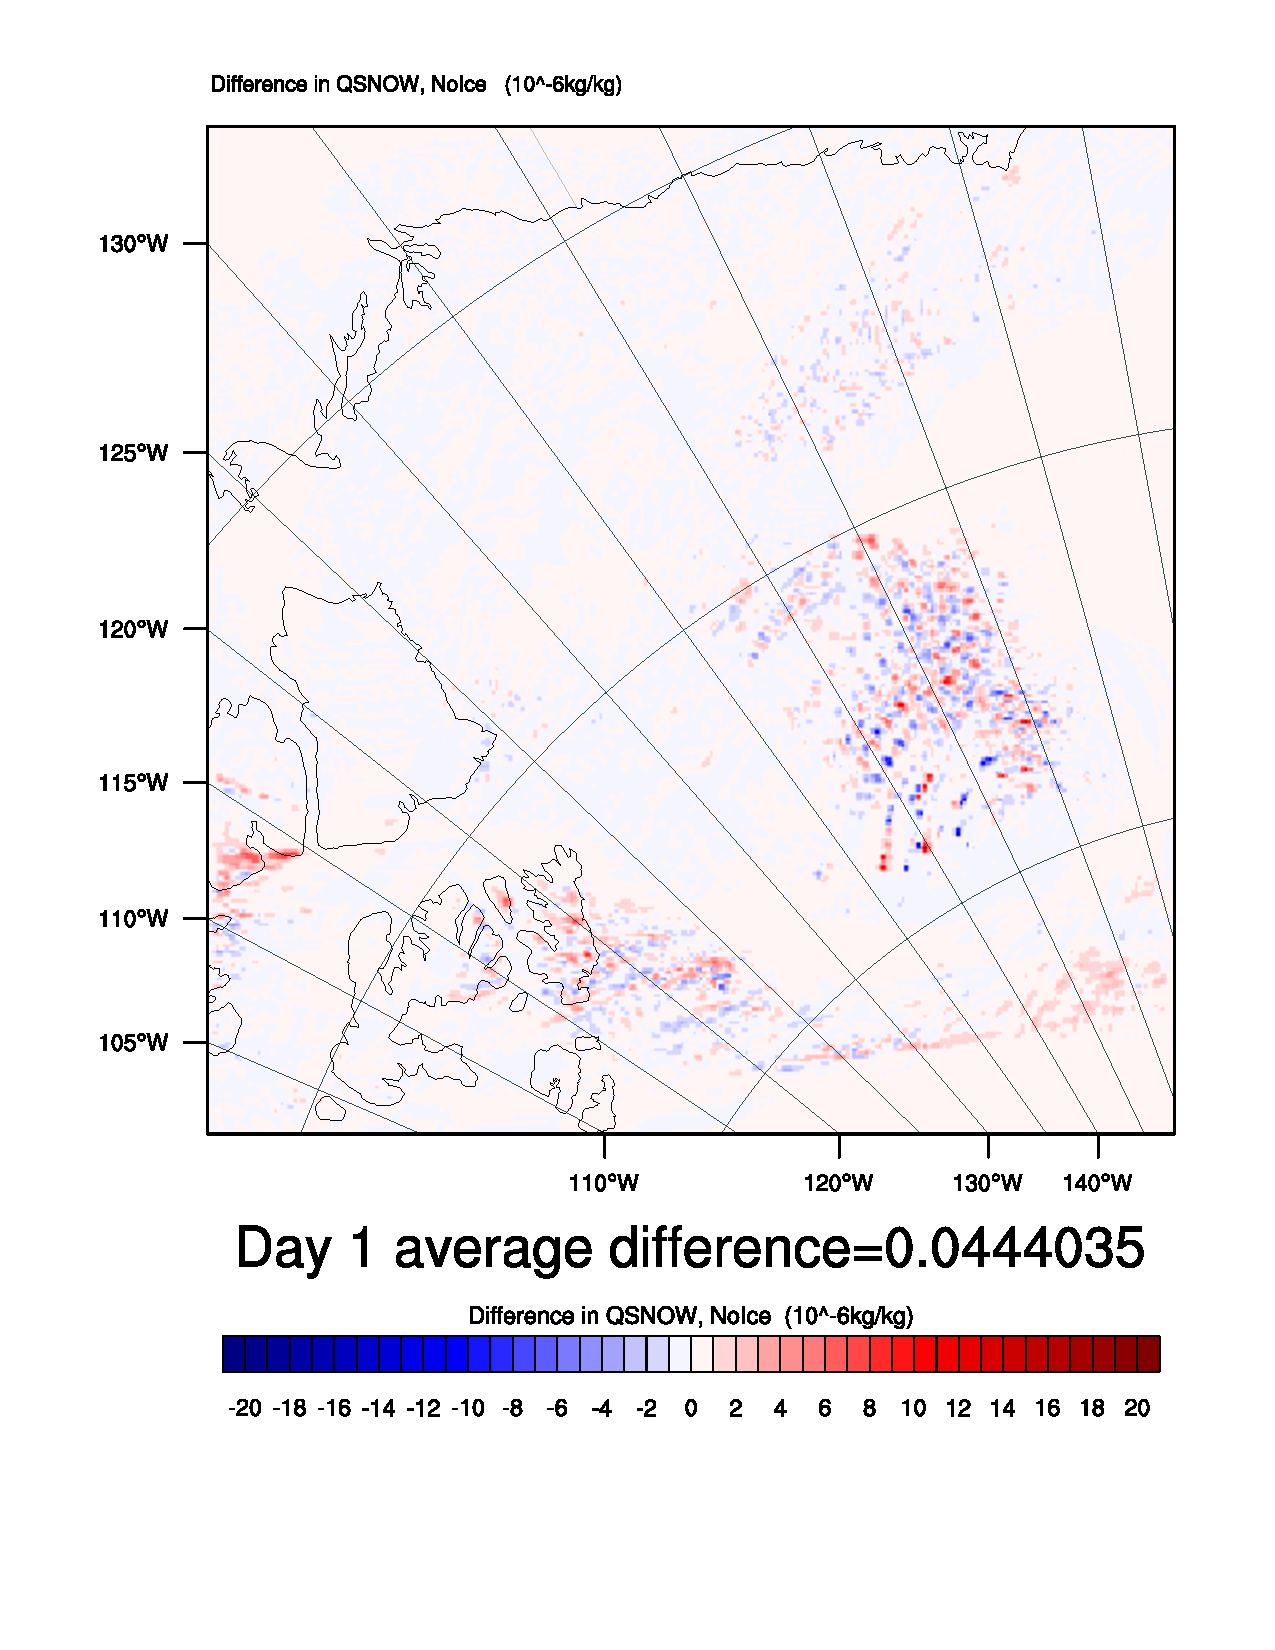
\includegraphics[width=\textwidth]{results/noice/diff_NoIce_qsnow_Day1.pdf}
		\caption{Day 1}
		\label{subfig:snowstory_Day1}
	\end{subfigure}
	\begin{subfigure}{0.32\textwidth}
		\centering
		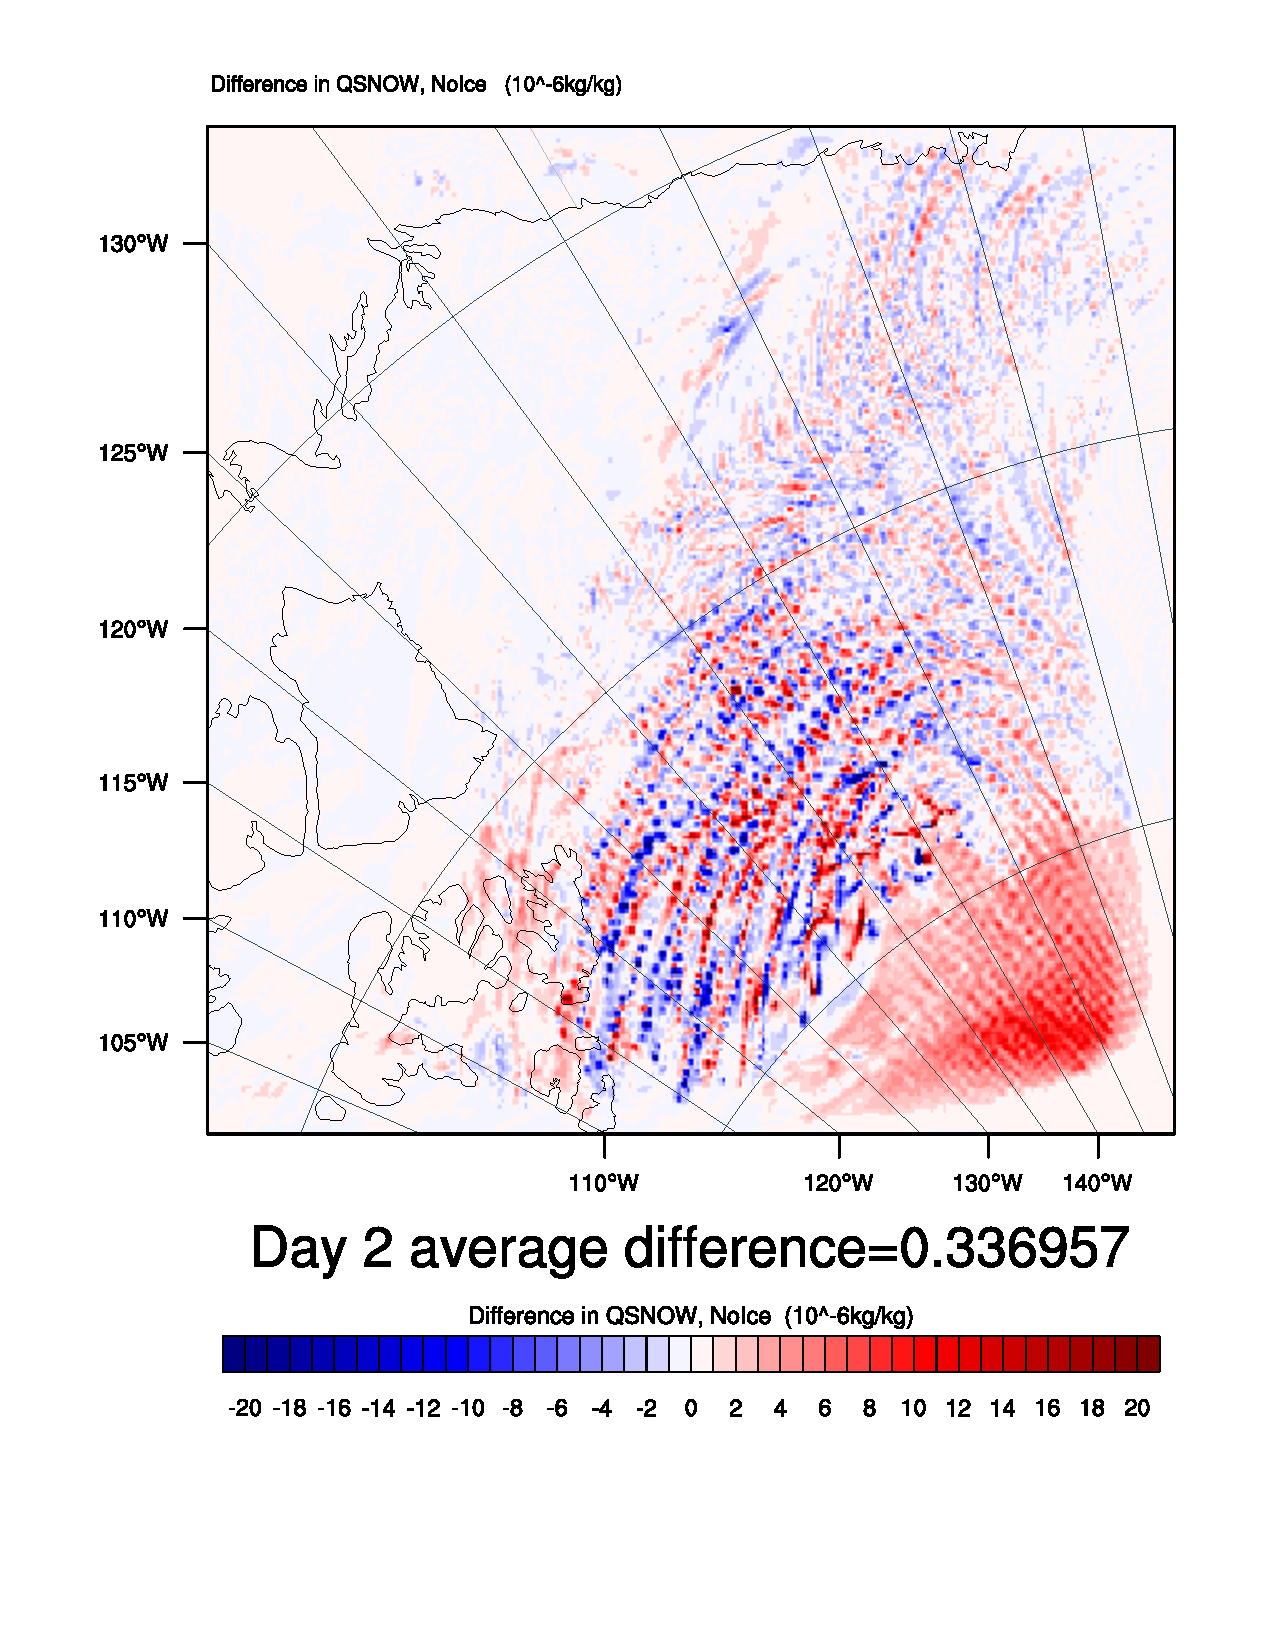
\includegraphics[width=\textwidth]{results/noice/diff_NoIce_qsnow_Day2.pdf}
		\caption{Day 2}
		\label{subfig:snowstory_Day2}
	\end{subfigure}
	\begin{subfigure}{0.32\textwidth}
		\centering
		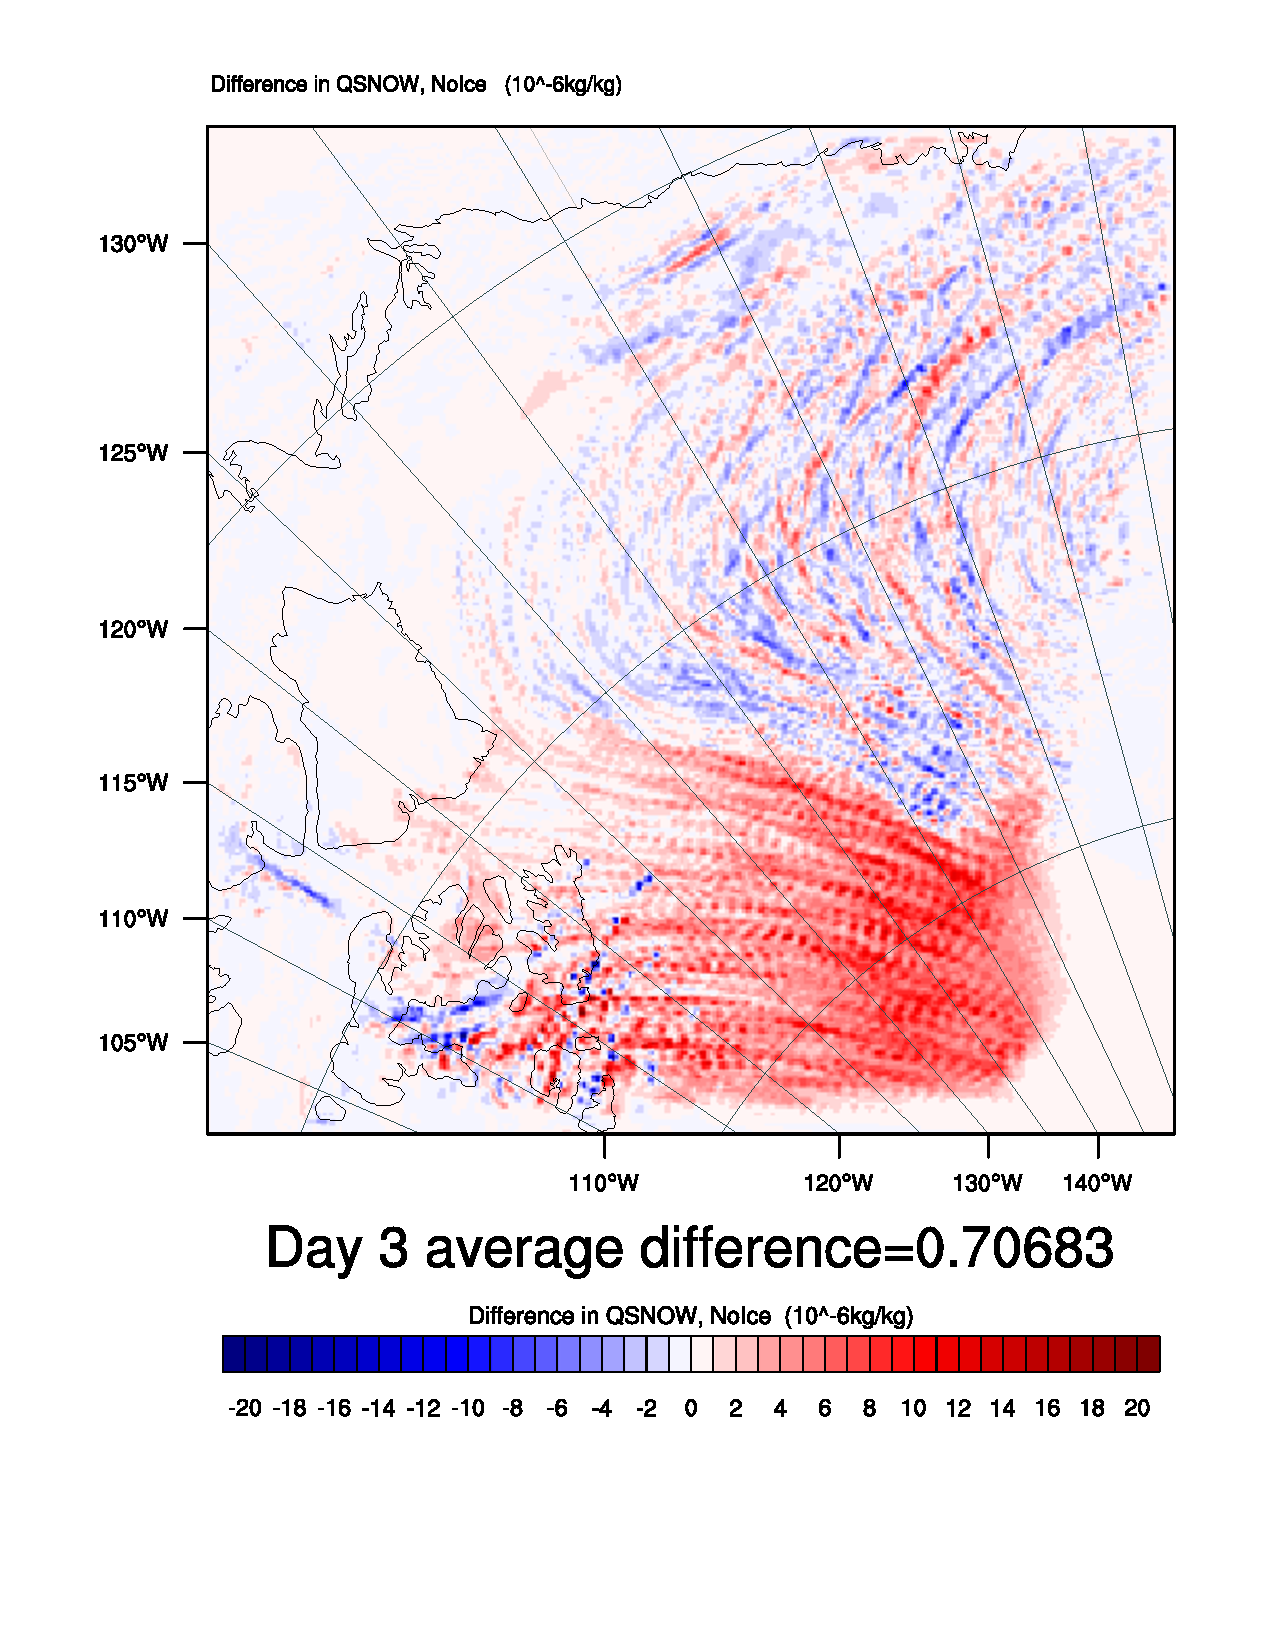
\includegraphics[width=\textwidth]{results/noice/diff_NoIce_qsnow_Day3.pdf}
		\caption{Day 3}
	\end{subfigure}

	\begin{subfigure}{0.32\textwidth}
		\centering
		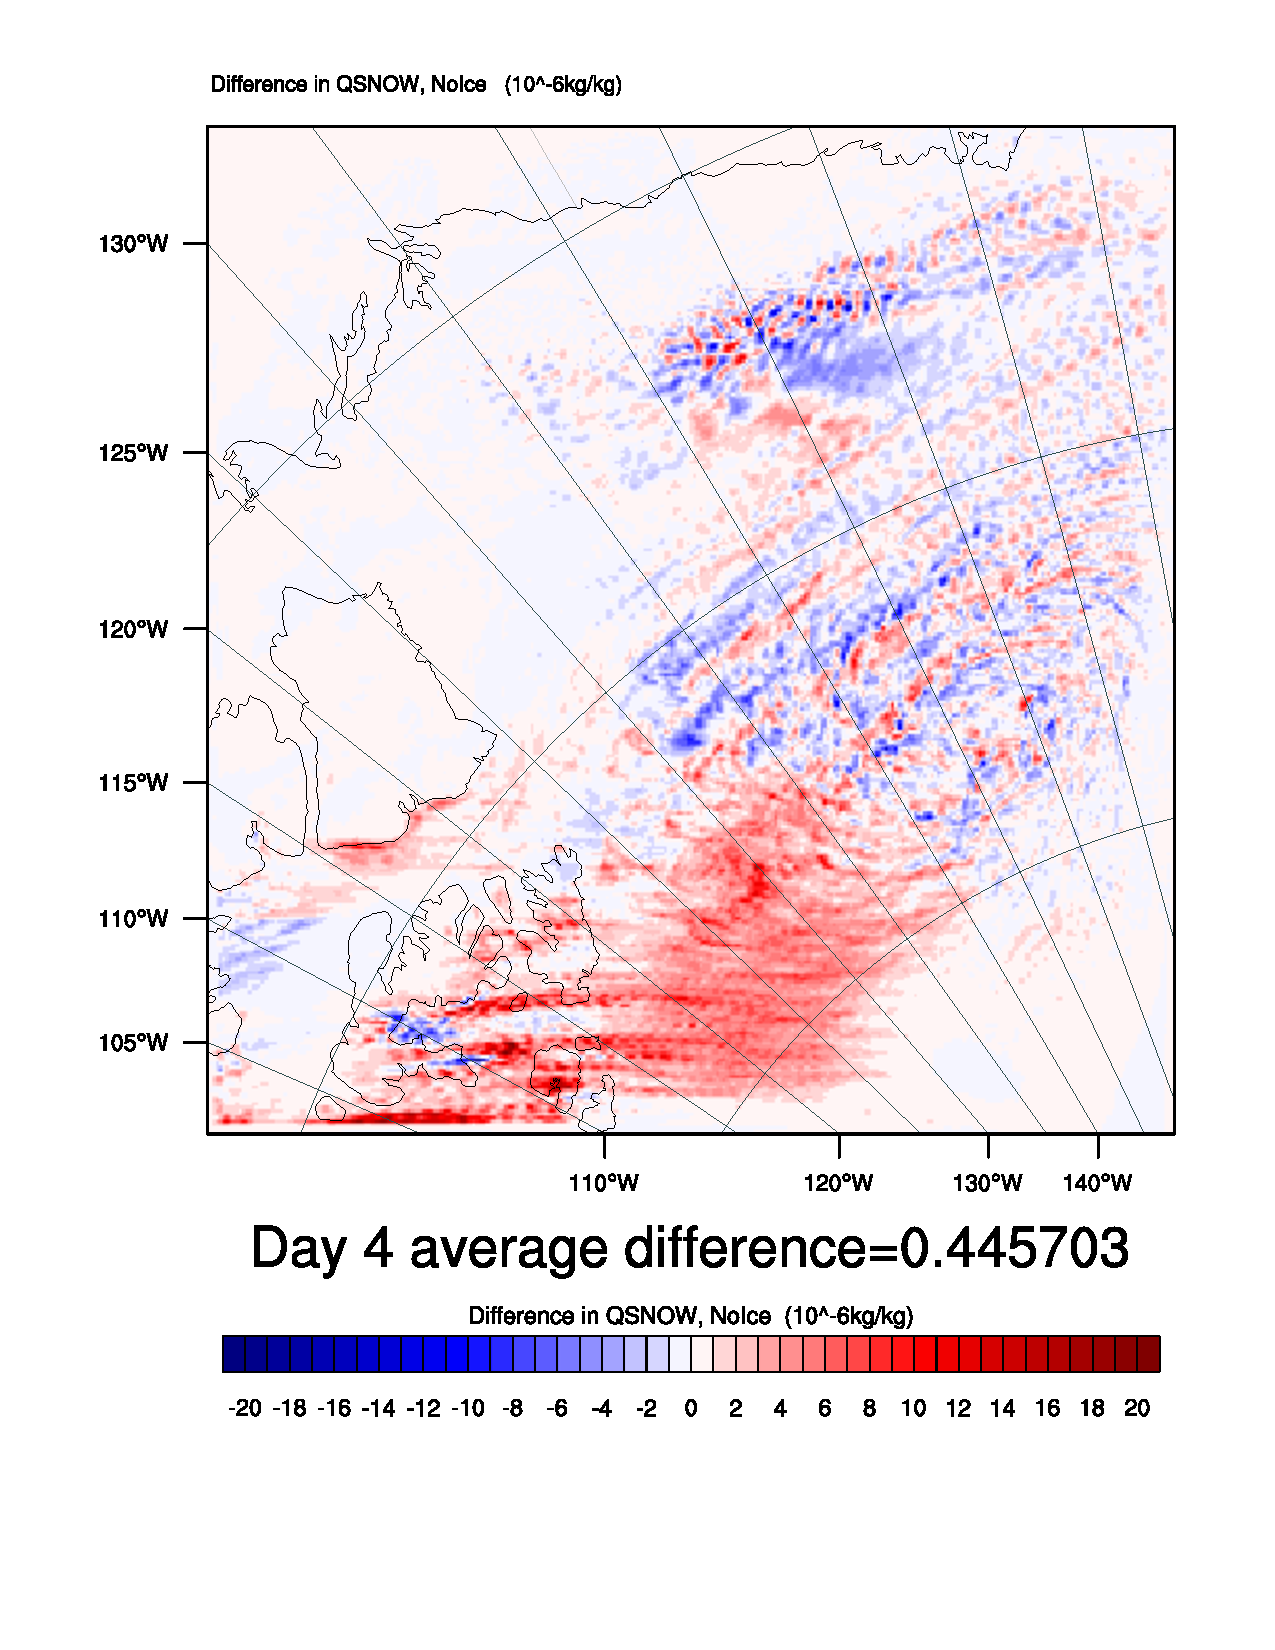
\includegraphics[width=\textwidth]{results/noice/diff_NoIce_qsnow_Day4.pdf}
		\caption{Day 4}
	\end{subfigure}
	\begin{subfigure}{0.32\textwidth}
		\centering
		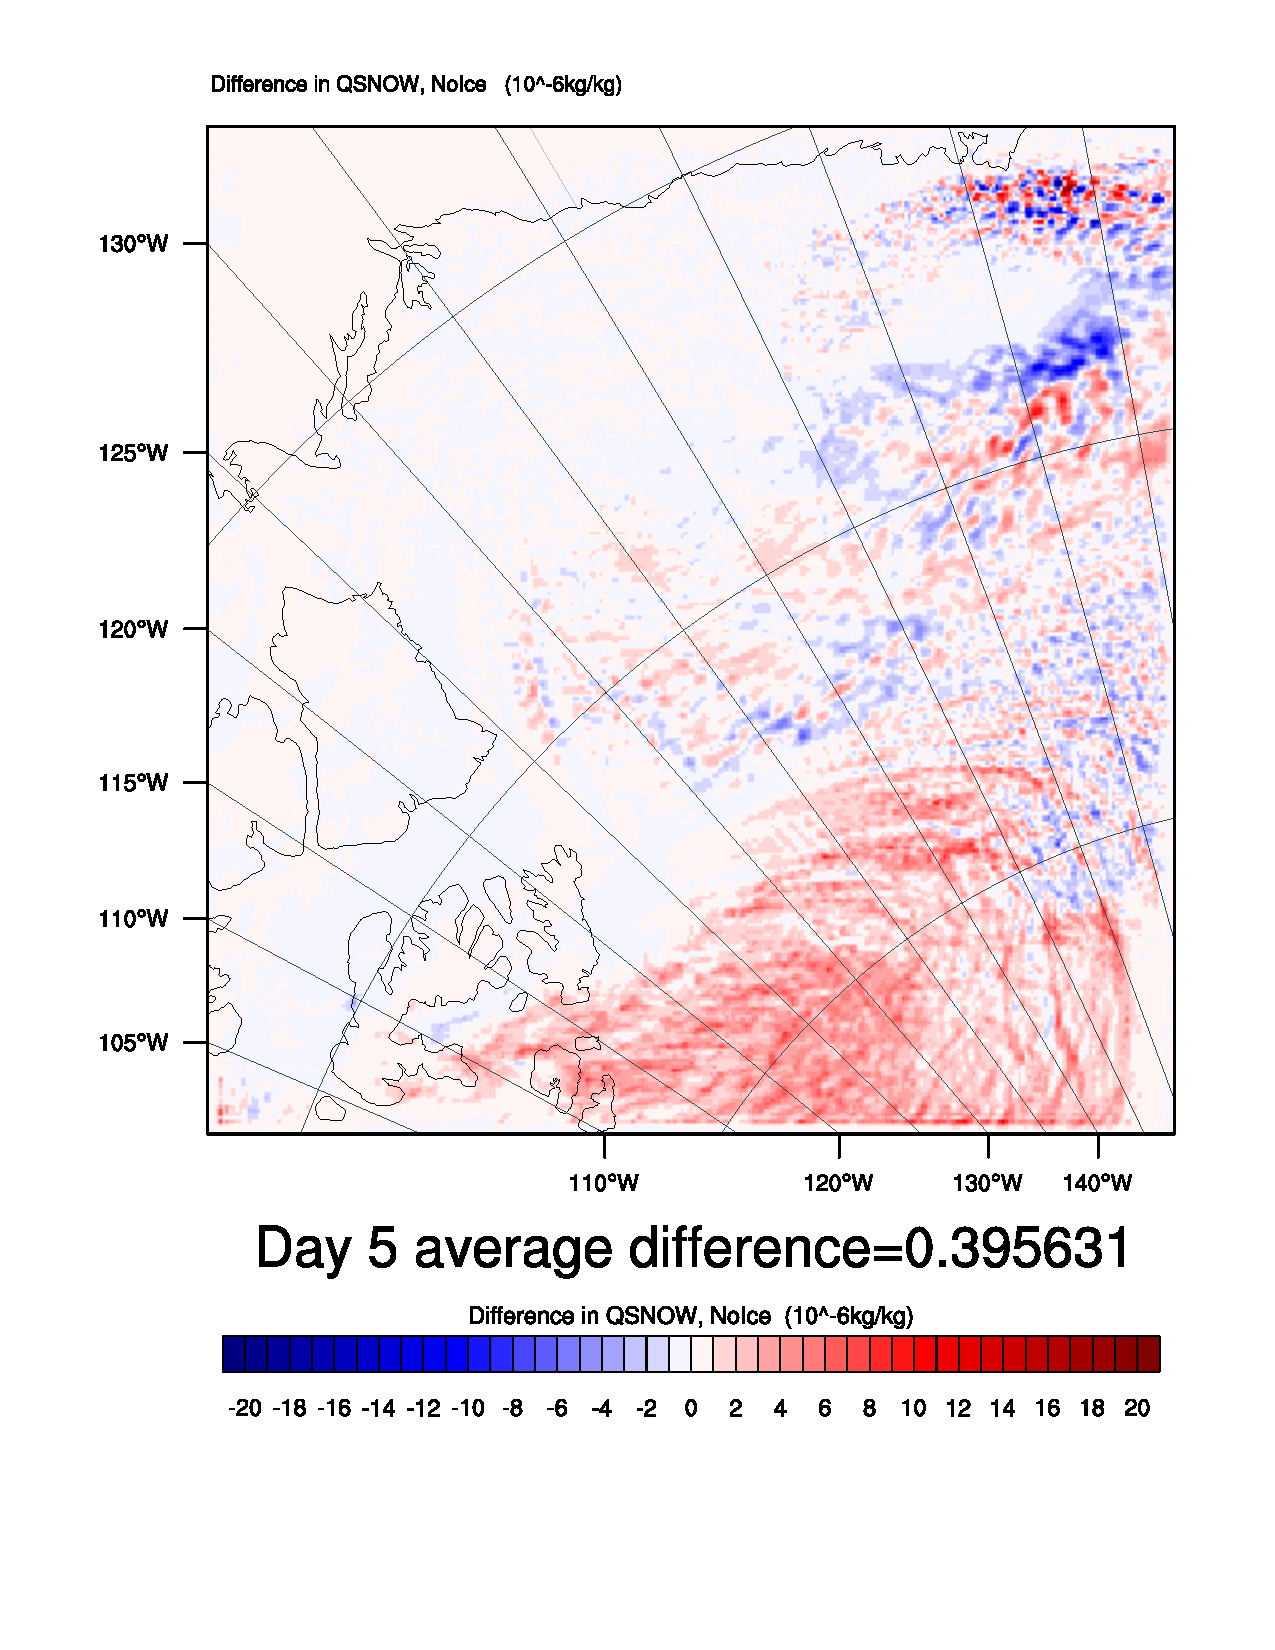
\includegraphics[width=\textwidth]{results/noice/diff_NoIce_qsnow_Day5.pdf}
		\caption{Day 5}
		\label{subfig:snowstory_Day5}
	\end{subfigure}
\caption{The average difference in mixing ratio of snow to air, over the lowermost 11 layers for days 1 to 5. NoIce-Control.}
\label{fig:snowstory}
\end{figure}

Figure~\ref{subfig:snowstory_Day1} shows the difference in mixing ratio of snow to air averaged for day 1 over the 11 lowermost layers. The slight increase in mixing ratio of snow is in the same area as the red patch in figure~\ref{subfig:CDNCr2Day5} that was claimed to be a forming cloud. Figure~\ref{subfig:snowstory_Day2} shows that in day 2 the cloud has indeed formed and it starts its journey south-eastward and continues through to day 5, see figure~\ref{subfig:snowstory_Day5} where the positive difference in snow is less pronounced, but still present.

The clouds on the 5th day of the run with no ice are now significantly thinner than the clouds in the 5th day of the control run, due to the aforementioned reduction in CDNC. This allows for more of the upwelling LW at TOA to come directly from the surface, which holds a higher temperature than the atmosphere above (see cross section in figure~\ref{subfig:cross_LWC_Day5}) and the newly ice free area also has a higher skin temperature, an increase of $\sim$1$\degree$C than the area did in the control run, when there was sea ice there (see figure~\ref{subfig:skin_r2Day5}). Following Stefan-Boltzmann's law (equation~\ref{eqn:stefanboltzmann}) the surface should now emit more LW than the clouds and sea ice with lower temperatures in the control run did. Figure~\ref{subfig:lwup_r2Day5} shows that the upwelling LW at TOA has indeed increased by $\sim$0.5 to 5 $\text{W/m}^2$ over the area where sea ice has been removed. Overall the average increase in upwelling LW at TOA for the whole area is just shy of 0.5, but the area of particular interest is where the sea ice has been removed, and that shows a more pronounced difference than the rest of the field.

\begin{figure}
\centering
	\begin{subfigure}{0.48\textwidth}
		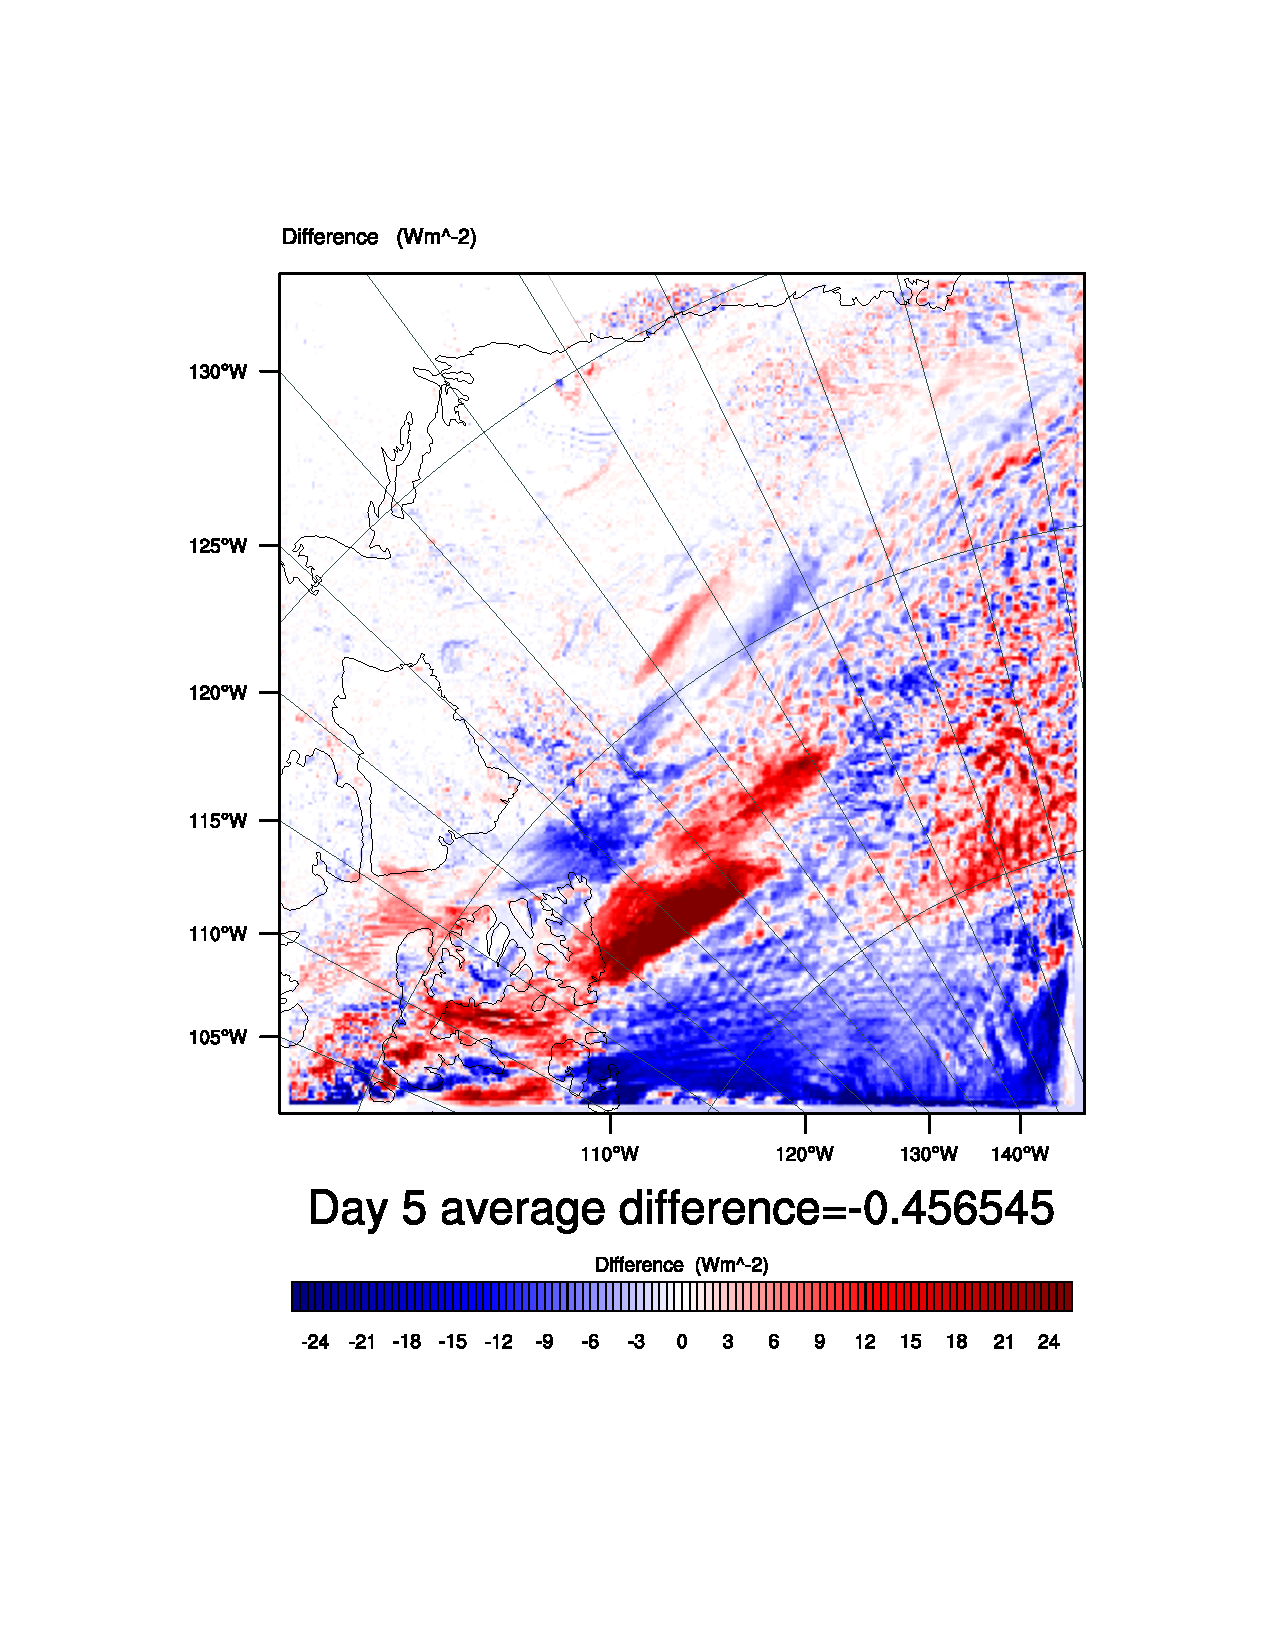
\includegraphics[width=\textwidth]{results/noice/diff_NoIce_SWDOWN_Day5.pdf}
		\caption{The average difference in SW flux down at the surface, day 5.}
		\label{subfig:swdown_r2Day5}
	\end{subfigure}
	\quad
	\begin{subfigure}{0.48\textwidth}
		\centering
		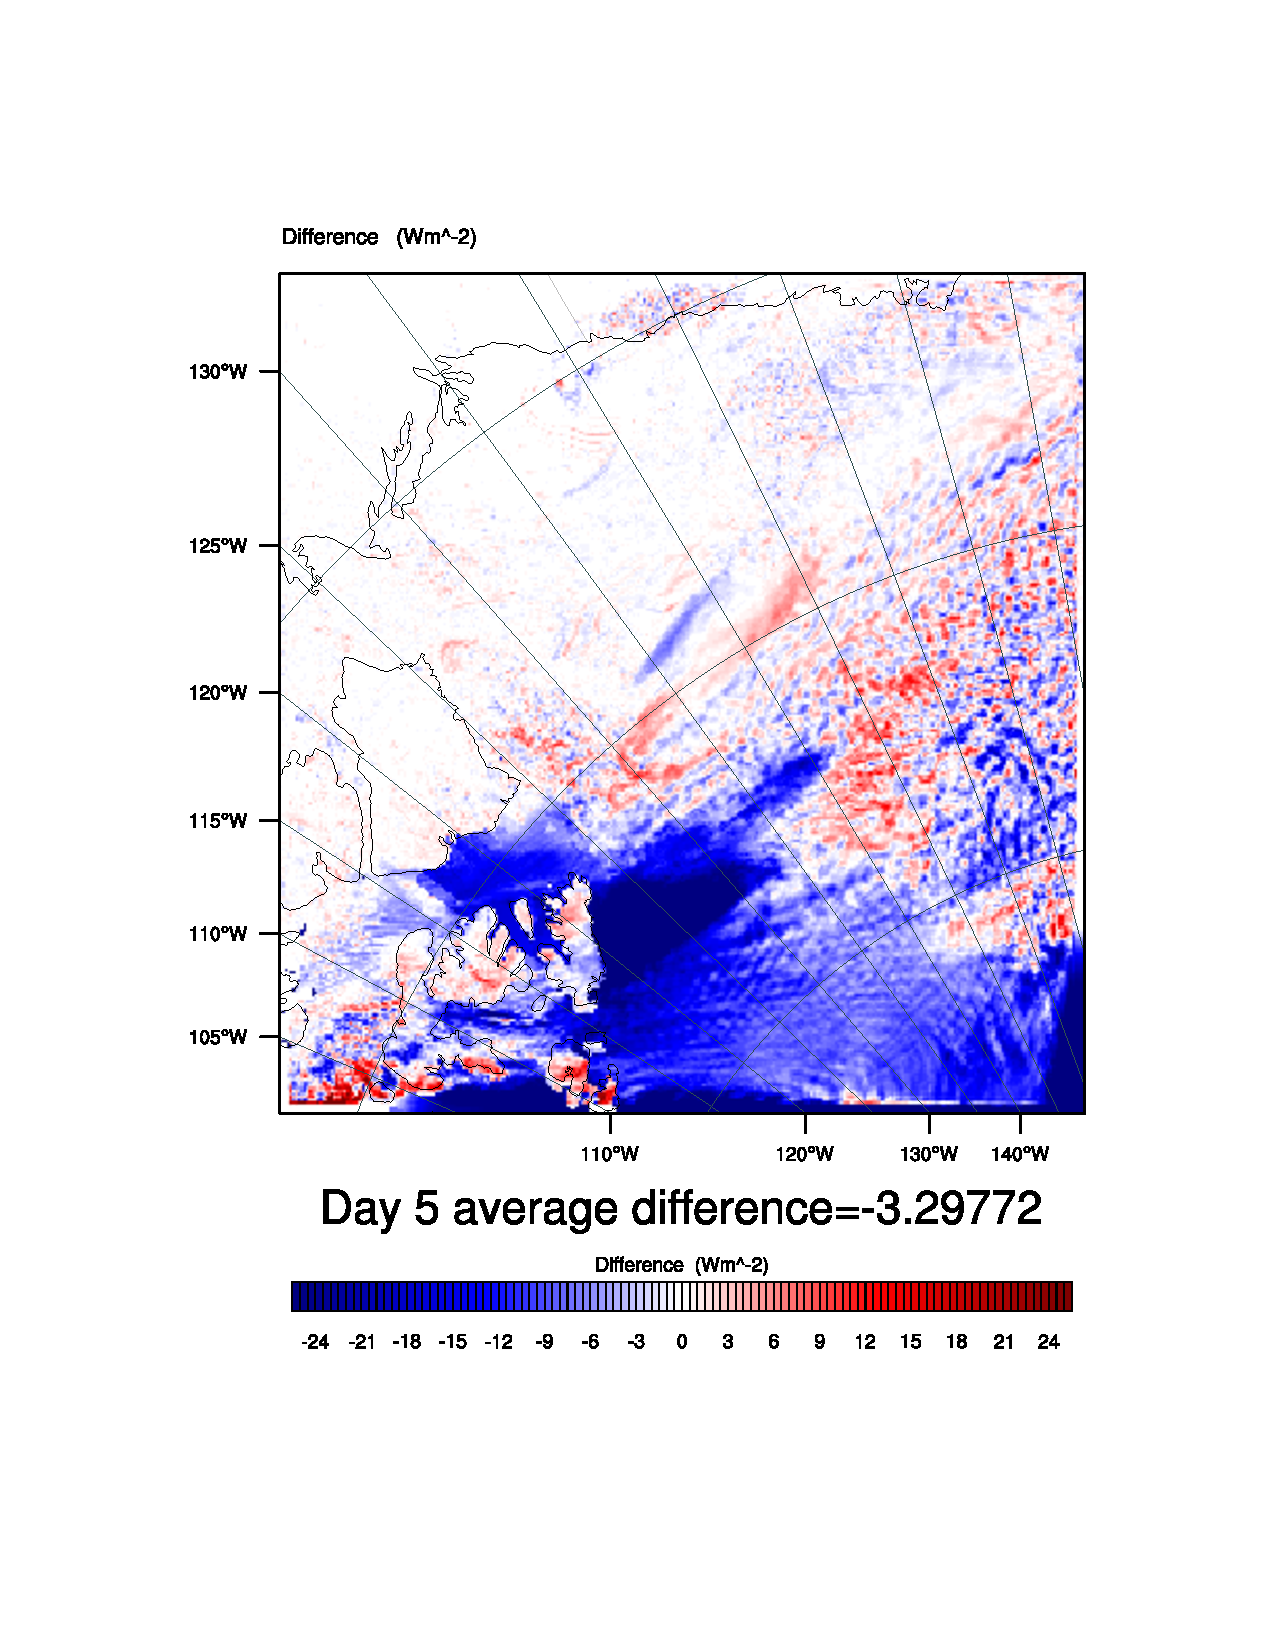
\includegraphics[width=\textwidth]{results/noice/diff_NoIce_SWUPT_Day5.pdf}
		\caption{The average difference in SW flux up at TOA, day 5.}
		\label{subfig:swup_r2Day5}
	\end{subfigure}
	
	\begin{subfigure}{0.48\textwidth}
		\centering
		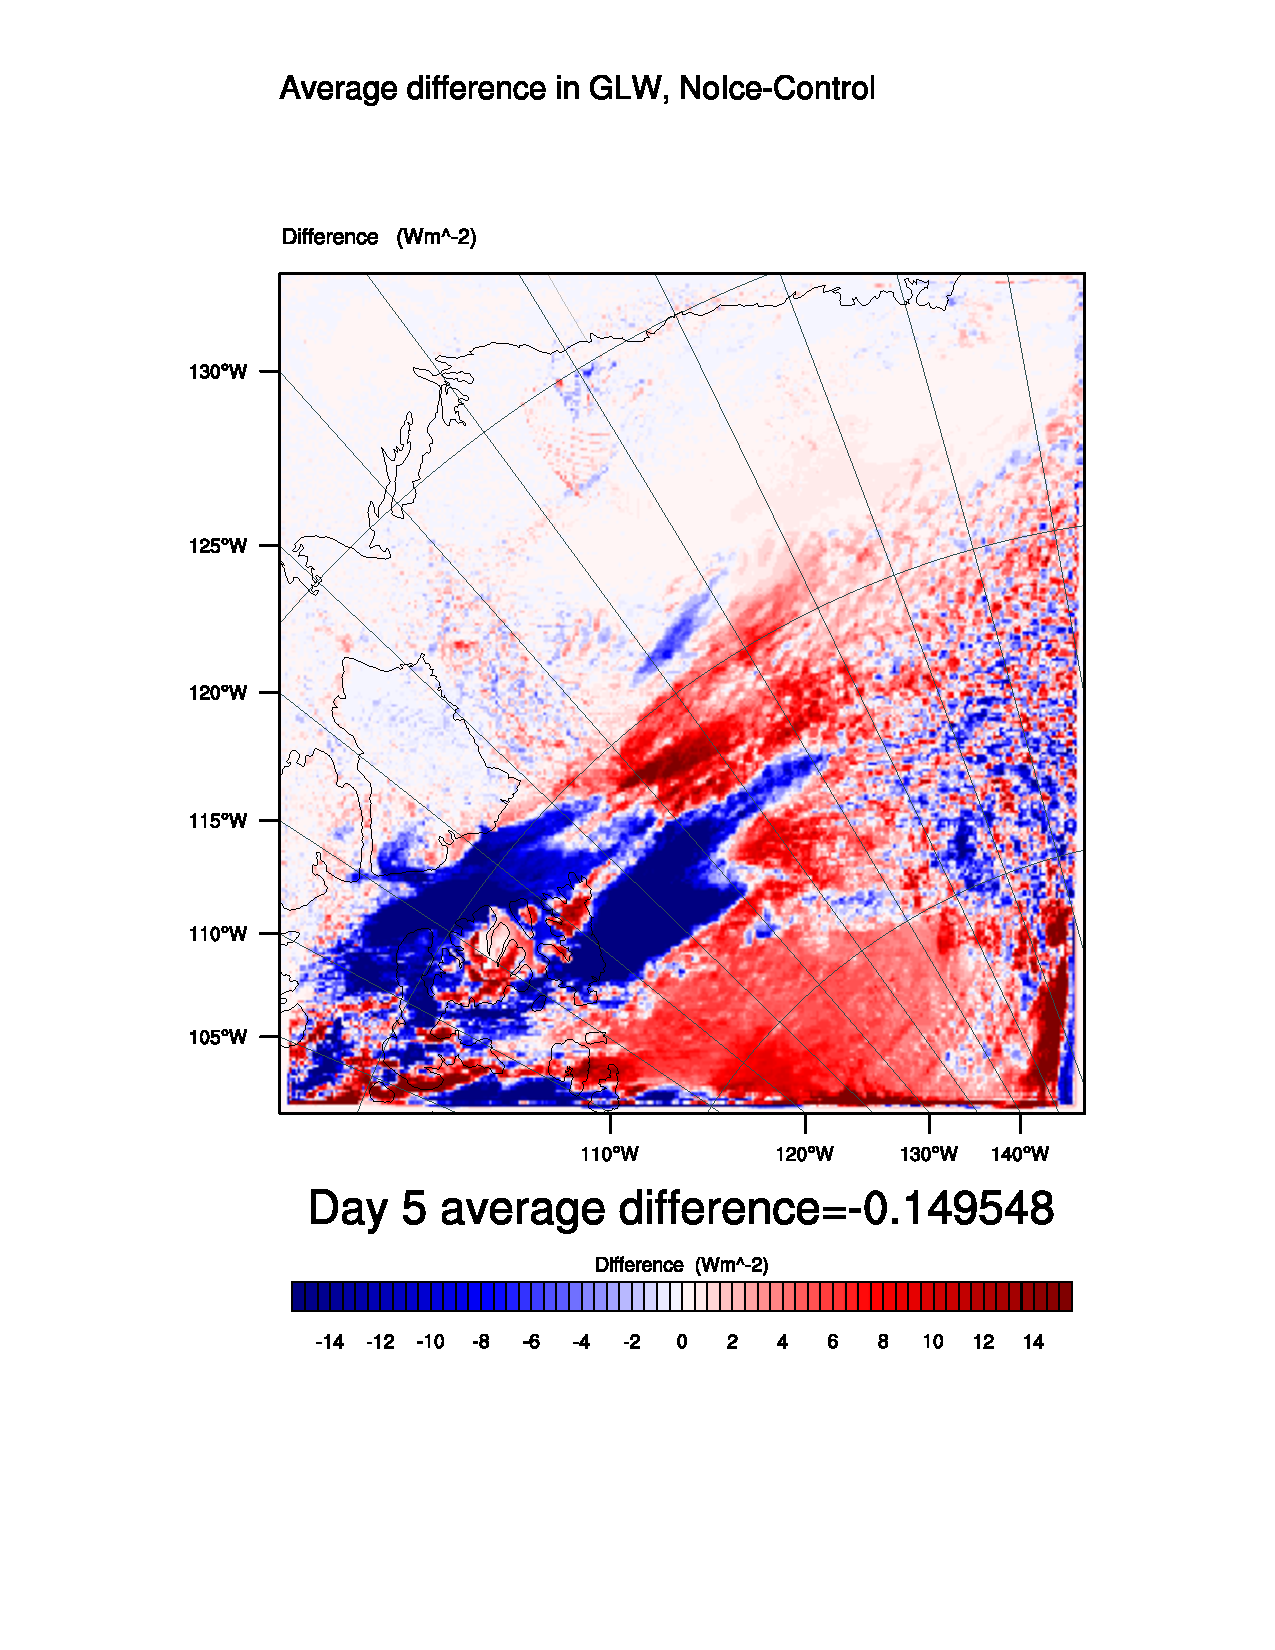
\includegraphics[width=\textwidth]{results/noice/diff_NoIce_GLW_Day5.pdf}
		\caption{The average difference in LW flux down at the surface, day 5.}
		\label{subfig:glw_r2Day5}
	\end{subfigure}
	\quad
	\begin{subfigure}{0.48\textwidth}
		\centering
		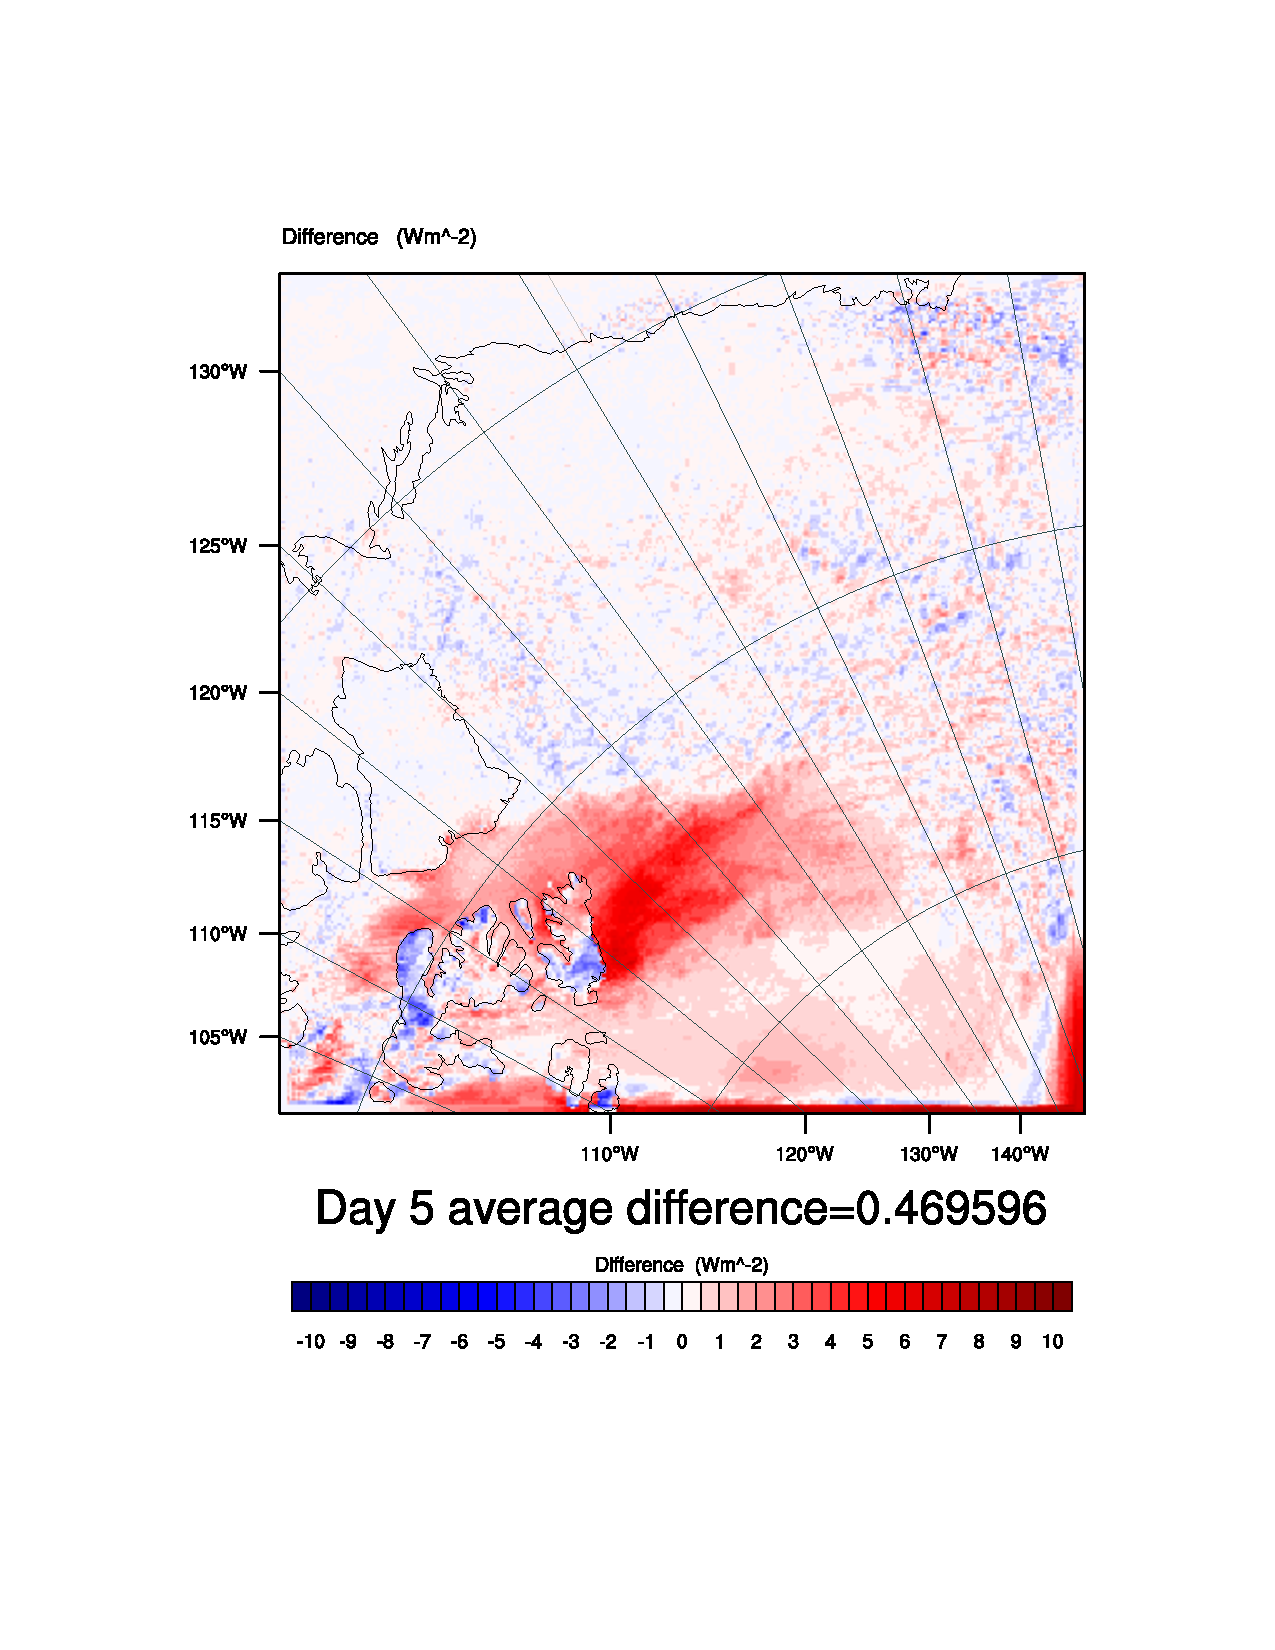
\includegraphics[width=\textwidth]{results/noice/diff_NoIce_LWUPT_Day5.pdf}
		\caption{The average difference in LW flux up at TOA, day 5.}
		\label{subfig:lwup_r2Day5}
	\end{subfigure}
	\caption{The average difference in SW and LW flux down at the surface and up at TOA, for day 5. NoIce-Control.}
	\label{fig:radiation_r2Day5}
\end{figure}

In figure~\ref{fig:radiation_r2Day5} the difference, for NoIce-Control, in SW down at the surface and up at TOA is illustrated by figures~\ref{subfig:swdown_r2Day5} and~\ref{subfig:swup_r2Day5}. The upwelling SW at TOA (figure~\ref{subfig:swup_r2Day5}) has an average difference of $\sim$~-3.3~$\text{W/m}^2$ for the whole field, and from <-25 to around -10~$\text{W/m}^2$ over the now ice free area. Such a decrease in upwelling SW radiation over the whole area that was covered by sea ice in the control run is because of the significant decrease in albedo of the area (not shown), which was discussed under day 1. The most pronounced decrease in upwelling SW at TOA at 77$\degree$N and 125$\degree$W is of same size and shape as the equally pronounced increase in downwelling SW at the surface of >25~$\text{W/m}^2$ (figure~\ref{subfig:swdown_r2Day5}), in the same place. This can also be recognized as the most significant decrease in CDNC which has lost more than 5 droplets~$\text{cm}^{-3}$ (figure~\ref{subfig:CDNCr2Day5}) compared to the control run. Thus, a cloud that was there in the control run has been significantly thinned or ceased to exist completely, such a decrease in CDNC ($N$ in equation~\ref{eqn:cloudtau1}) decreases the cloud optical depth, $\tau$, and albedo, $A$ (equation~\ref{eqn:cloudalbedo}), and does therefore not protect the surface from downwelling SW by reflecting it back to TOA.

The red patch at 77$\degree$N stretching from 120 to 140$\degree$W, in figure~\ref{subfig:swdown_r2Day5}, indicating the increase in downwelling SW is recognized as a decrease in downwelling LW in the same area in figure~\ref{subfig:glw_r2Day5}. This can also be explained by the decrease in CDNC, or rather the LWP, where if the clouds are thinned or cease to exist, the LW emissivity of the clouds would decrease as the LWP decreased (equation~\ref{eqn:epsilon_lw}), provided the LWP got lower than 40-45~$\text{g/m}^2$ according to figure~\ref{fig:epsalb}. Looking at the difference in LWP in figure~\ref{subfig:LWPr2Day5}, which shows LWP for NoIce-Control, one sees that the LWP in NoIce is >30~$\text{g/m}^2$ less than in the control run for that exact area. The LWP in the control run (figure~\ref{subfig:LWPr1Day5}) for that area was 30 to 60~$\text{g/m}^2$. Thus the LWP in NoIce is below the limit for saturation on LW and the LW emissivity is decreased, explaining the decrease in LW reaching the surface in that particular area.

For quite a large part of the area which is now sea ice free the downwelling LW experiences an increase compared to the control run, difference shown in figure~\ref{subfig:glw_r2Day5}. The depletion of clouds by snow, decreasing the LWP, would intuitively also decrease the downwelling LW at the surface if one considers the decrease in emissivity it would lead to, based on equation~\ref{eqn:epsilon_lw}. On the other hand, knowing Stefan-Boltzmann's law (equation~\ref{eqn:stefanboltzmann}) the temperature of the emitting body is of crucial importance. The removal of sea ice has led to an increase in surface heat fluxes and skin temperature, as mentioned in day 1, and shows the same for day 5 in figure~\ref{fig:lhshskin_r2Day5}.

\begin{figure}
\centering
	\begin{subfigure}{0.48\textwidth}
		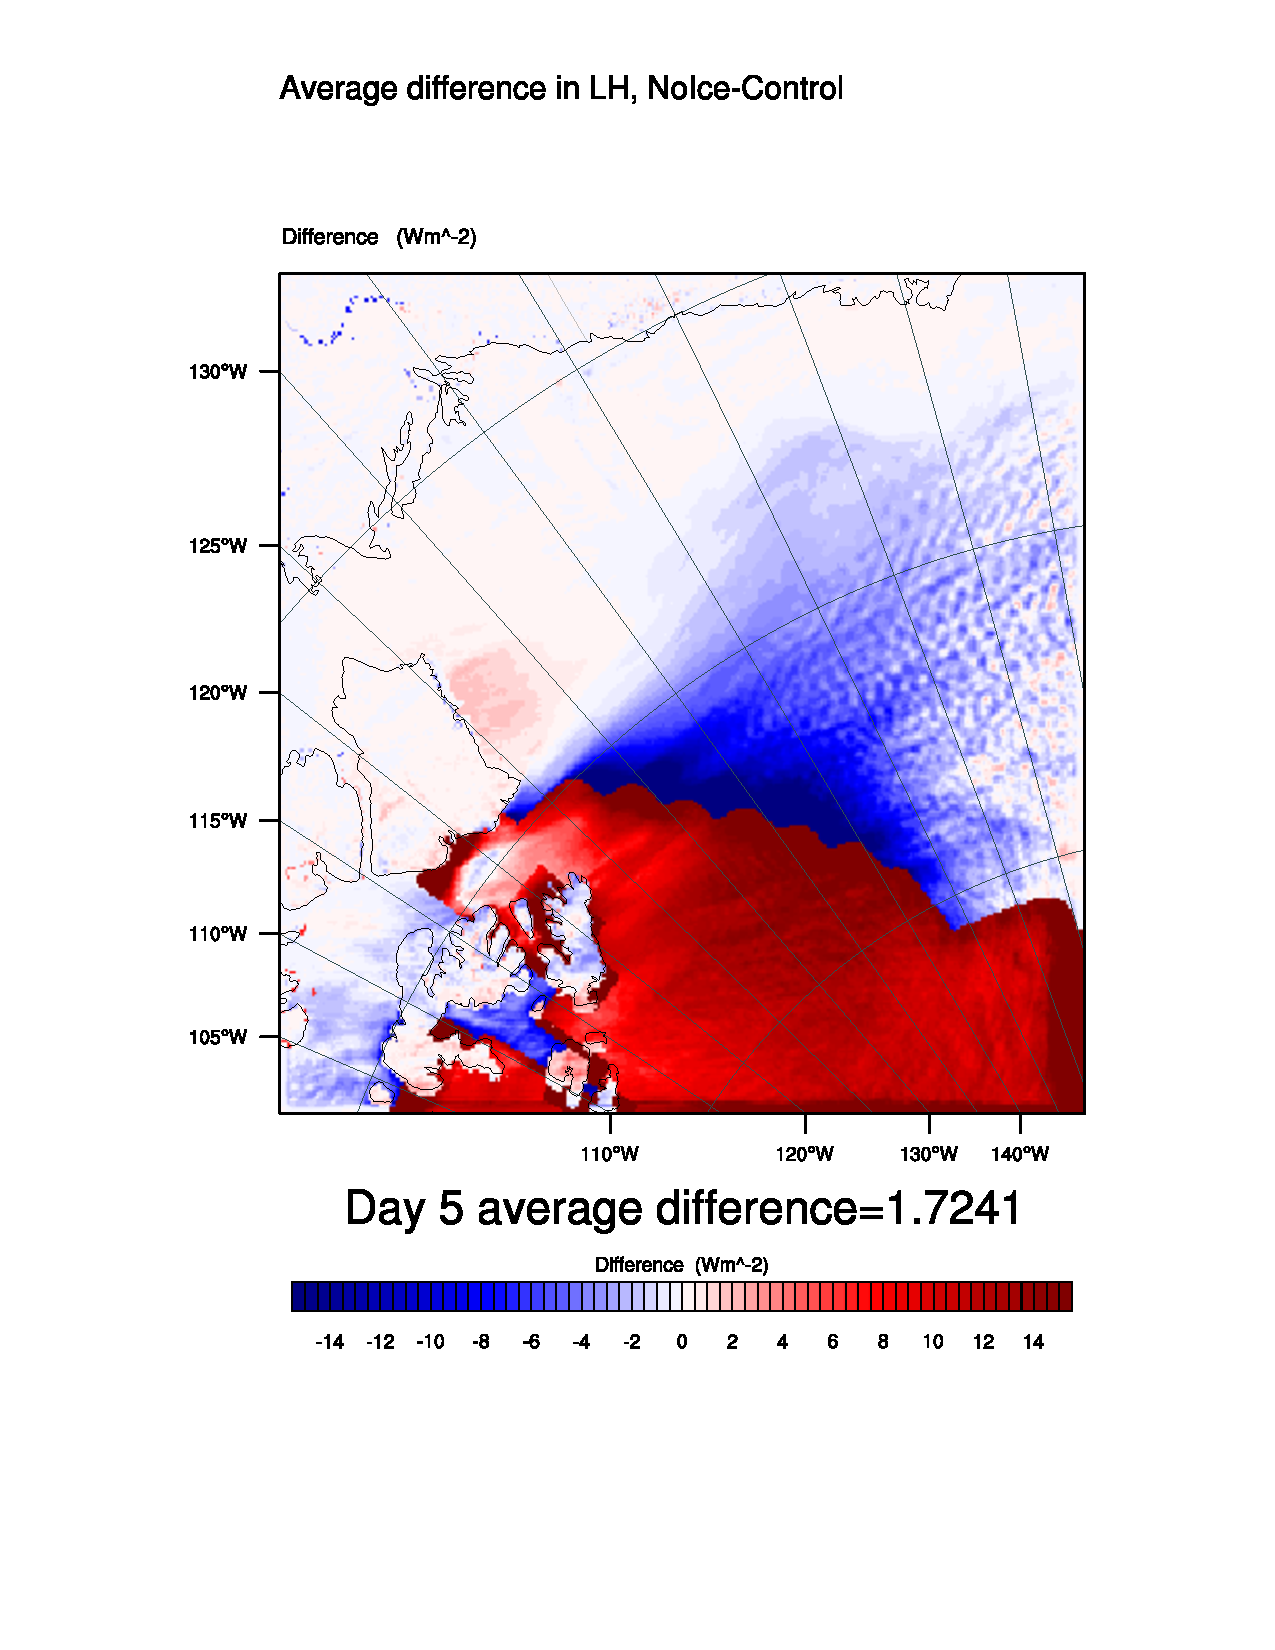
\includegraphics[width=\textwidth]{results/noice/diff_NoIce_LH_Day5.pdf}
		\caption{Difference in LH.}
		\label{subfig:lh_r2Day5}
	\end{subfigure}
	\quad
		\begin{subfigure}{0.48\textwidth}
		\includegraphics[width=\textwidth]{results/noice/diff_NoIce_HFX_Day5.pdf}
		\caption{Difference in SH.}
		\label{subfig:sh_r2Day5}
	\end{subfigure}
	
	\begin{subfigure}{0.48\textwidth}
		\includegraphics[width=\textwidth]{results/noice/diff_NoIce_skintemp_Day5.pdf}
		\caption{Difference in skin temperature.}
		\label{subfig:skin_r2Day5}
	\end{subfigure}
	\caption{Average difference in LH, SH and skin temperature for day 5. NoIce-Control.}
	\label{fig:lhshskin_r2Day5}
\end{figure}

A higher skin temperature and increased surface heat fluxes pushes the lower cloud limit slightly higher up into the atmosphere, the cloud height for a section of the area can be seen in the vertical cross section for LWC on day 5~\ref{fig:cross_LWC_r2Day5} for the run with no ice. Comparing this with the vertical cross section from the control run, figure~\ref{subfig:cross_LWC_Day5}, it is clear that the stratus clouds lie approximately 500~m higher closer to the mountain in the NoIce run than they did in the control run.

\begin{figure}
\centering
\includegraphics[width=0.6\textwidth]{results/noice/crossSec_LWC_NoIce_Day5.pdf}
\caption{Averaged LWC in the NoIce run for day 5, in the vertical cross section over the red line in figure~\ref{subfig:cross_line}.}
\label{fig:cross_LWC_r2Day5}
\end{figure}

Looking at vertical cross sections from NoIce and Control the clouds seem to have the same temperature in both runs, but in NoIce the cloud does not stretch as close to the mountain as in Control, and between 100 and 120 on the x-axis NoIce has no cloud, which fits with the decrease in downwelling LW in that area (77$\degree$N and 117$\degree$W). The increase in downwelling LW on the other hand might be explained by the increase in cloud height. .....\textit{men den forklaringen er jeg veldig usikker paa, se e-post}

%-------------------------------------
\clearpage
\section{Increased aerosol number concentration}
%-------------------------------------
The aerosol number concentration was multiplied by 10 to study the effects of pollution in the area. The increased ship traffic in the Arctic @(cite Kari?) leads to higher aerosol load which could affect the cloud radiative properties, and thereby have a warming or cooling effect at the surface. Figure%~\ref{fig:aerosol} 
shows the aerosol concentration for Control and for Aero10, where the pattern obviously is the same, and overall increased by a factor of 10 (notice the different scales).

%\begin{figure}[hb]
%\centering
%	\begin{subfigure}{0.48\textwidth}
%		\centering
%		\includegraphics[width=\textwidth]{}
%		\caption{QNWFA, Control}
%		\label{subfig:qnwfa_r1}
%	\end{subfigure}
%	\begin{subfigure}{0.48\textwidth}
%		\centering
%		\includegraphics[width=\textwidth]{}
%		\caption{QNWFA, Aero10}
%		\label{subfig:qnwfa_r1}
%	\end{subfigure}
%\caption{Aerosols, both water and ice-friendly. In Control and Aero10.}
%\end{figure}


\subsection{Day 1}
With an aerosol number concentration 10 times higher than that in the control run, the average LWP and CDNC for day1 increase by about 11~$\text{g/m}^2$ and 16~$\text{cm}^{-3}$ respectively, see figure~\ref{fig:lwpcdncre_r3Day1}. The increases in CDNC and LWP are expected with such a high increase in available CCN. Remembering the first indirect effect described in Chapter~\ref{chap:theory}, one would expect a decrease in droplet size with the increase in numbers. $r_e$ has in fact decreased for the whole field in this run, and is shown in figure~\ref{subfig:recloud_r3Day1}

\begin{figure}[hb]
\centering
	\begin{subfigure}{0.40\textwidth}
		\centering
		\includegraphics[width=\textwidth]{results/aero10/Diff_LWP_Day1Aero10.pdf}
		\caption{LWP, Aero10, day 1}
		\label{subfig:LWPr3Day1}
	\end{subfigure}
	\quad
	\begin{subfigure}{0.40\textwidth}
		\centering
		\includegraphics[width=\textwidth]{results/aero10/diff_Aero10_QNCLOUD_Day1.pdf}
		\caption{CDNC, Aero10, day 1}
		\label{subfig:CDNCr3Day1}
	\end{subfigure}
	
	\begin{subfigure}{0.40\textwidth}
		\centering
		\includegraphics[width=\textwidth]{results/aero10/diff_Aero10_RE_CLOUD_Day1.pdf}
		\caption{$r_e$, Aero10, day 1}
		\label{subfig:recloud_r3Day1}
	\end{subfigure}
\caption{The averaged difference in LWP, CDNC and $r_e$ of cloud droplets (from left to right) over the lowermost 11 layers for day 1. Aero10-Control.}
\label{fig:lwpcdncre_r3Day1}
\end{figure}

The first indirect effect describes an increase in the cloud albedo as a consequence of more numerous and smaller droplets, and the upwelling SW at TOA is increased by as much as $\sim$7~$\text{W/m}^2$ on average for the whole field on day 1 (see figure~\ref{subfig:swup_r3Day1}). As opposed to the run with no ice, the sea ice is unchanged in the run with increased aerosol number concentration (Aero10), so the signal here is clearly an increase in reflected SW. Over the sea ice however the increase in reflected SW is not as large as in the rest of the field, since the sea ice already has a relatively high albedo itself (around 0.6). The increase in the albedo of the clouds has significantly reduced the downwelling SW at the surface (figure~\ref{subfig:swdown_r3Day1}) compared to the control run. The change is $\sim$9~$\text{W/m}^2$ decrease on average for the study area, which represents a cooling. On the other hand the average LW radiation at the surface is higher (figure~\ref{subfig:glw_r3Day1}) due to the aforementioned increase in LWP and thereby increased emittance by the clouds, as follows from equation~\ref{eqn:epsilon_lw}. The increase in LW reaching the surface is $\sim$2.3~$\text{W/m}^2$. The most pronounced increase in LW at the surface is in areas where the LWP in the control run (figure~\ref{subfig:LWPr1Day1}) was lower and therefore not as close to saturation with respect to cloud LW emissivity. Two of these areas are 79$\degree$N, 135-140$\degree$W and 82$\degree$N, 125-135$\degree$W. 

\begin{figure}
\centering
	\begin{subfigure}{0.48\textwidth}
		\includegraphics[width=\textwidth]{results/aero10/diff_Aero10_SWDOWN_Day1.pdf}
		\caption{The average difference in SW flux down at the surface, day 1.}
		\label{subfig:swdown_r3Day1}
	\end{subfigure}
	\quad
	\begin{subfigure}{0.48\textwidth}
		\centering
		\includegraphics[width=\textwidth]{results/aero10/diff_Aero10_SWUPT_Day1.pdf}
		\caption{The average difference in SW flux up at TOA, day 1.}
		\label{subfig:swup_r3Day1}
	\end{subfigure}
	
	\begin{subfigure}{0.48\textwidth}
		\centering
		\includegraphics[width=\textwidth]{results/aero10/diff_Aero10_GLW_Day1.pdf}
		\caption{The average difference in LW flux down at the surface, day 1.}
		\label{subfig:glw_r3Day1}
	\end{subfigure}
	\quad
	\begin{subfigure}{0.48\textwidth}
		\centering
		\includegraphics[width=\textwidth]{results/aero10/diff_Aero10_LWUPT_Day1.pdf}
		\caption{The average difference in LW flux up at TOA, day 1.}
		\label{subfig:lwup_r3Day1}
	\end{subfigure}
	\caption{The average difference in SW and flux down at the surface and up at TOA, for day 1. Aero10-Control.}
	\label{fig:radiation_r3Day1}
\end{figure}

There is no clear response in the surface heat fluxes to the increased aerosol number concentration(not shown).

%-----------------
\clearpage
\subsection{Day 5}
%-----------------
The differences in LWP and CDNC and $r_e$ for day 5 (Aero10-Control) are shown in figure~\ref{fig:lwpcdncre_r3Day5}. As for day 1, the LWP shows an average increase for the whole study area. The increase in LWP on day 5 in Aero10 compared to Control is $\sim$20~$\text{g/m}^2$ and is especially high where the LWP was also high in the control run (see figure~\ref{subfig:LWPr1Day5}). The increase in CDNC has the same pattern as the increase in LWP, which is expected based on equation~\ref{eqn:LWC}. The average increase in CDNC for the study area is $\sim$22~$\text{cm}^{-3}$. Similarly to day 1, evidence of the first indirect effect is suspected since $r_e$ has an average decrease of $\sim$0.6~$\mu\text{m}$, which means that still for day 5 there are more numerous and smaller droplets. Also for $r_e$ the pattern is the same as for LWP, but with opposite sign.
\begin{figure}[hb]
\centering
	\begin{subfigure}{0.30\textwidth}
		\centering
		\includegraphics[width=\textwidth]{results/aero10/Diff_LWP_Day5Aero10.pdf}
		\caption{LWP, Aero10, day 5}
		\label{subfig:LWPr3Day5}
	\end{subfigure}
	\begin{subfigure}{0.30\textwidth}
		\centering
		\includegraphics[width=\textwidth]{results/aero10/diff_Aero10_QNCLOUD_Day5.pdf}
		\caption{CDNC, Aero10, day 5}
		\label{subfig:CDNCr3Day5}
	\end{subfigure}
	\begin{subfigure}{0.30\textwidth}
		\centering
		\includegraphics[width=\textwidth]{results/aero10/diff_Aero10_RE_CLOUD_Day5.pdf}
		\caption{$r_e$, Aero10, day 5}
		\label{subfig:recloud_r3Day5}
	\end{subfigure}
	\caption{The averaged difference in LWP, CDNC and $r_e$ of cloud droplets (from left to right) over the lowermost 11 layers for day 5. Aero10-Control.}
	\label{fig:lwpcdncre_r3Day5}
\end{figure}

The LW cloud emissivity is sensitive to an increase in water amount as long as the LWP is less than $\sim$40-45~$\text{g/m}^2$. Day 5 in the control run had LWP around 60-100~$\text{g/m}^2$ in the middle lower area of figure~\ref{subfig:LWPr1Day5}. %@ (around these lat and lon?@).
This is also seen in that there is no significant change in LW downward at the surface or upward at the TOA, see figures~\ref{subfig:glw_r3Day5} and~\ref{subfig:lwup_r3Day5}.

\begin{figure}
\centering
	\begin{subfigure}{0.48\textwidth}
		\includegraphics[width=\textwidth]{results/aero10/diff_Aero10_SWDOWN_Day5.pdf}
		\caption{The average difference in SW flux down at the surface, day 5.}
		\label{subfig:swdown_r3Day5}
	\end{subfigure}
	\quad
	\begin{subfigure}{0.48\textwidth}
		\centering
		\includegraphics[width=\textwidth]{results/aero10/diff_Aero10_SWUPT_Day5.pdf}
		\caption{The average difference in SW flux up at TOA, day 5.}
		\label{subfig:swup_r3Day5}
	\end{subfigure}
	
	\begin{subfigure}{0.48\textwidth}
		\centering
		\includegraphics[width=\textwidth]{results/aero10/diff_Aero10_GLW_Day5.pdf}
		\caption{The average difference in LW flux down at the surface, day 5.}
		\label{subfig:glw_r3Day5}
	\end{subfigure}
	\quad
	\begin{subfigure}{0.48\textwidth}
		\centering
		\includegraphics[width=\textwidth]{results/aero10/diff_Aero10_LWUPT_Day5.pdf}
		\caption{The average difference in LW flux up at TOA, day 5.}
		\label{subfig:lwup_r3Day5}
	\end{subfigure}
	\caption{The average difference in SW and LW flux down at the surface and up at TOA, for day 5. Aero10-Control.}
	\label{fig:radiation_r3Day5}
\end{figure}

The area with lack of change in LW up or down is approximately the same area as where there is a negative change in LH and SH upward from the surface over the sea ice, see figure \ref{fig:lhshskin_r3Day5}. Since there has been no change in LW there is no loss of warming from a decrease in LW reaching the surface, but the change can be explained by looking at the SW radiation. The downward SW at the surface has been significantly decreased as a consequence of the increase in aerosol number concentration, see figure~\ref{subfig:swdown_r3Day5}. This is known as the first indirect effect, and was described in Chapter~\ref{chap:theory}. 
\begin{figure}
\centering
	\begin{subfigure}{0.48\textwidth}
		\includegraphics[width=\textwidth]{results/aero10/diff_Aero10_LH_Day5.pdf}
		\caption{Difference in LH.}
		\label{subfig:lh_r3Day5}
	\end{subfigure}
	\quad
	\begin{subfigure}{0.48\textwidth}
		\includegraphics[width=\textwidth]{results/aero10/diff_Aero10_HFX_Day5.pdf}
		\caption{Difference in SH.}
		\label{subfig:sh_r3Day5}
	\end{subfigure}

	\begin{subfigure}{0.48\textwidth}
		\includegraphics[width=\textwidth]{results/aero10/diff_Aero10_TSK_Day5.pdf}
		\caption{Difference in skin temperature.}
		\label{subfig:skin_r3Day5}
	\end{subfigure}
	\caption{Average difference in LH, SH and skin temperature for day1. Aero10-Control.}
	\label{fig:lhshskin_r3Day5}
\end{figure}
The albedo of the sea ice in Aero10 is around 0.6 (not shown) which means that a fraction of the incident SW radiation is absorbed. Since the amount of incident SW radiation at the surface has been reduced by the cloud cover, the absorbed radiation is less than for a higher incident amount. The ice therefore has a lower temperature to give off SH with. 

%Look at temperature changes at the surface. Over ice and ocean.. 
The skin temperature, figure~\ref{subfig:skin_r3Day5}, for the domain shows a small decrease in the same area as where there is less sensible and latent heat release.

%Also the dynamics over ice and the ocean are different, so this could have an effect. The cold air over the ice may be intensified, while the sea surface temperature (SST) is the same for all the runs and there is no coupling with the ocean. There will therefore be no changes in the SSTs that could have an effect on the dynamics over the ocean. So the response may be smaller there...?

%------------
\clearpage
\section{Removed sea ice \underline{and}~increased aerosol}
%------------
The effects on radiative cloud properties and the surface by removal of sea ice and increased aerosol number concentration is studied combined. This is to get an idea of the effects of increased pollution from sea traffic as a consequence of more ice free ocean, in combination with more available heat and moisture from the ocean. @cite someone looking at that and what they found? The results in this section are not discussed as detailed as the results presented in the two previous sections for NoIce and Aero10 separately. This is to avoid too much repetition of the mechanisms behind the differences.

%-----------------
\subsection{Day 1}
%-----------------
The difference in LWP between the run with both removed sea ice and incerased aerosol number concentration (Aero10NoIce) and Control for day 1 (figure~\ref{subfig:LWPr4Day1}) is clearly due to the increase is number of aerosols. The increase in LWP for day 1 in NoIce (figure~\ref{subfig:LWPr2Day1}) was on average $\sim$0.2~$\text{g/m}^2$ for the whole field, whereas for Aero10 it was 11~$\text{g/m}^2$, which is also the average increase for Aero10NoIce. The average increase in CDNC (figure~\ref{subfig:CDNCr4Day1}) for Aero10NoIce is also similar to Aero10 (figure~\ref{subfig:CDNCr3Day1}) where both those runs had an average increase of $\sim$15.9~$\text{cm}^{-3}$. The difference in effective radius is also the same with an average decrease in droplet size of about 0.5~$\mu\text{m}$ (see figure~\ref{subfig:recloud_r4Day1} for Aero10NoIce and~\ref{subfig:recloud_r3Day1} for Aero10). For these specific parameters it is clear that the effect of increasing the aerosol number concentration outweighs that of removing the sea ice.

% Figure with LWP, CDNC and r_e
\begin{figure}[hb]
\centering
	\begin{subfigure}{0.40\textwidth}
		\centering
		\includegraphics[width=\textwidth]{results/aero10ni/Diff_LWP_Day1Aero10NoIce.pdf}
		\caption{LWP}
		\label{subfig:LWPr4Day1}
	\end{subfigure}
	\quad
	\begin{subfigure}{0.40\textwidth}
		\centering
		\includegraphics[width=\textwidth]{results/aero10ni/diff_Aero10NoIce_QNCLOUD_Day1.pdf}
		\caption{CDNC}
		\label{subfig:CDNCr4Day1}
	\end{subfigure}
	
	\begin{subfigure}{0.40\textwidth}
		\centering
		\includegraphics[width=\textwidth]{results/aero10ni/diff_Aero10NoIce_RE_CLOUD_Day1.pdf}
		\caption{$r_e$}
		\label{subfig:recloud_r4Day1}
	\end{subfigure}
\caption{The averaged difference in LWP, CDNC and $r_e$ of cloud droplets (from left to right) over the lowermost 11 layers for day 1. Aero10NoIce-Control.}
\label{fig:lwpcdncre_r4Day1}
\end{figure}

When looking at the difference in radiation fluxes down at the surface and up at TOA (figure~\ref{fig:radiation_r4Day1}) one can see that both the removal of sea ice and the increase in aerosol number concentration make a difference.  For downward SW at the surface (figure~\ref{subfig:swdown_r4Day1}) the average difference can be interpreted as a sum of the difference in NoIce and Aero10. NoIce and Aero10 had average decreases in SW down of $\sim$2.36~$\text{W/m}^2$ (figure~\ref{subfig:swdown_r2Day1}) and $\sim$9.25~$\text{W/m}^2$ (figure~\ref{subfig:swdown_r3Day1}) respectively. When added together they are almost equal to the average difference in Aero10NoIce, which is a decrease of 11.6~$\text{W/m}^2$. Such a decrease in downwelling SW radiation could have a cooling effect at the surface. It can be seen from figures~\ref{subfig:lh_r4Day1},~\ref{subfig:sh_r4Day1} and~\ref{subfig:skin_r4Day1} showing LH, SH and skin temperature respectively, that there is a decrease in upward surface fluxes and temperature of the surface at 77-79$\degree$N and 115-125$\degree$W, which fits perfectly with the area of most pronounced decrease in downwelling SW in figure~\ref{subfig:swdown_r4Day1}.

% Figure with SW and LW down at surface and up at TOA
\begin{figure}
\centering
	\begin{subfigure}{0.48\textwidth}
		\includegraphics[width=\textwidth]{results/aero10ni/diff_Aero10NoIce_SWDOWN_Day1.pdf}
		\caption{SW down at surface.}
		\label{subfig:swdown_r4Day1}
	\end{subfigure}
	\quad
	\begin{subfigure}{0.48\textwidth}
		\centering
		\includegraphics[width=\textwidth]{results/aero10ni/diff_Aero10NoIce_SWUPT_Day1.pdf}
		\caption{SW up at TOA.}
		\label{subfig:swup_r4Day1}
	\end{subfigure}
	
	\begin{subfigure}{0.48\textwidth}
		\centering
		\includegraphics[width=\textwidth]{results/aero10ni/diff_Aero10NoIce_GLW_Day1.pdf}
		\caption{LW down at surface.}
		\label{subfig:glw_r4Day1}
	\end{subfigure}
	\quad
	\begin{subfigure}{0.48\textwidth}
		\centering
		\includegraphics[width=\textwidth]{results/aero10ni/diff_Aero10NoIce_LWUPT_Day1.pdf}
		\caption{LW up at TOA.}
		\label{subfig:lwup_r4Day1}
	\end{subfigure}
	\caption{The average difference in SW and LW flux down at the surface and up at TOA, for day 1. Aero10NoIce-Control.}
	\label{fig:radiation_r4Day1}
\end{figure}

% Figure with LH, SH and skintemp
\begin{figure}
\centering
	\begin{subfigure}{0.48\textwidth}
		\includegraphics[width=\textwidth]{results/aero10ni/diff_Aero10NoIce_LH_Day1.pdf}
		\caption{Difference in LH.}
		\label{subfig:lh_r4Day1}
	\end{subfigure}
	\quad
	\begin{subfigure}{0.48\textwidth}
		\includegraphics[width=\textwidth]{results/aero10ni/diff_Aero10NoIce_HFX_Day1.pdf}
		\caption{Difference in SH.}
		\label{subfig:sh_r4Day1}
	\end{subfigure}

	\begin{subfigure}{0.48\textwidth}
		\includegraphics[width=\textwidth]{results/aero10ni/diff_Aero10NoIce_TSK_Day1.pdf}
		\caption{Difference in skin temperature.}
		\label{subfig:skin_r4Day1}
	\end{subfigure}
	\caption{Average difference in LH and SH up at the surface, and difference in skin temperature, for day 1. Aero10NoIce-Control.}
	\label{fig:lhshskin_r4Day1}
\end{figure}

%-----------------
\clearpage
\subsection{Day 5}
%-----------------
% Figure with LWP, CDNC and r_e
\begin{figure}[hb]
\centering
	\begin{subfigure}{0.40\textwidth}
		\centering
		\includegraphics[width=\textwidth]{results/aero10ni/Diff_LWP_Day5Aero10NoIce.pdf}
		\caption{LWP}
		\label{subfig:LWPr4Day5}
	\end{subfigure}
	\quad
	\begin{subfigure}{0.40\textwidth}
		\centering
		\includegraphics[width=\textwidth]{results/aero10ni/diff_Aero10NoIce_QNCLOUD_Day5.pdf}
		\caption{CDNC}
		\label{subfig:CDNCr4Day5}
	\end{subfigure}
	
	\begin{subfigure}{0.40\textwidth}
		\centering
		\includegraphics[width=\textwidth]{results/aero10ni/diff_Aero10NoIce_RE_CLOUD_Day5.pdf}
		\caption{$r_e$}
		\label{subfig:recloudr4Day5}
	\end{subfigure}
\caption{The averaged difference in LWP, CDNC and $r_e$ of cloud droplets (from left to right) over the lowermost 11 layers for day 5. Aero10NoIce-Control.}
\label{fig:lwpcdncre_r4Day5}
\end{figure}

% Figure with SW and LW down at surface and up at TOA
\begin{figure}
\centering
	\begin{subfigure}{0.48\textwidth}
		\includegraphics[width=\textwidth]{results/aero10ni/diff_Aero10NoIce_SWDOWN_Day5.pdf}
		\caption{SW down at surface.}
		\label{subfig:swdown_r4Day5}
	\end{subfigure}
	\quad
	\begin{subfigure}{0.48\textwidth}
		\centering
		\includegraphics[width=\textwidth]{results/aero10ni/diff_Aero10NoIce_SWUPT_Day5.pdf}
		\caption{SW up at TOA.}
		\label{subfig:swup_r4Day5}
	\end{subfigure}
	
	\begin{subfigure}{0.48\textwidth}
		\centering
		\includegraphics[width=\textwidth]{results/aero10ni/diff_Aero10NoIce_GLW_Day5.pdf}
		\caption{LW down at surface.}
		\label{subfig:glw_r4Day5}
	\end{subfigure}
	\quad
	\begin{subfigure}{0.48\textwidth}
		\centering
		\includegraphics[width=\textwidth]{results/aero10ni/diff_Aero10NoIce_LWUPT_Day5.pdf}
		\caption{LW up at TOA.}
		\label{subfig:lwup_r4Day5}
	\end{subfigure}
	\caption{The average difference in SW and LW flux down at the surface and up at TOA, for day 5. Aero10NoIce-Control.}
	\label{fig:radiation_r4Day5}
\end{figure}

% Figure with LH, SH and skintemp
\begin{figure}
\centering
	\begin{subfigure}{0.48\textwidth}
		\includegraphics[width=\textwidth]{results/aero10ni/diff_Aero10NoIce_LH_Day5.pdf}
		\caption{Difference in LH.}
		\label{subfig:lh_r4Day5}
	\end{subfigure}
	\quad
	\begin{subfigure}{0.48\textwidth}
		\includegraphics[width=\textwidth]{results/aero10ni/diff_Aero10NoIce_HFX_Day5.pdf}
		\caption{Difference in SH.}
		\label{subfig:sh_r4Day5}
	\end{subfigure}

	\begin{subfigure}{0.48\textwidth}
		\includegraphics[width=\textwidth]{results/aero10ni/diff_Aero10NoIce_TSK_Day5.pdf}
		\caption{Difference in skin temperature.}
		\label{subfig:skin_r4Day5}
	\end{subfigure}
	\caption{Average difference in LH and SH up at the surface, and difference in skin temperature, for day 5. Aero10NoIce-Control.}
	\label{fig:lhshskin_r4Day5}
\end{figure}

% Må også oppgi gjennomsnittsverdi for hele feltet (for å hjelpe leseren) og minimums og maksimumsverdiene?, siden de ikke er med på labalbaren...

%Jon Egill har avtalt eksamen 19. juni. Erik Berge er sensor! Hvem er intern?
